\documentclass[mathserif]{beamer}
\usepackage{beamerthemeshadow}
\usepackage{beamerthemesplit}
%\usetheme{shadow}
\usecolortheme{default}
\setbeamertemplate{footline}[frame number]
\useinnertheme[shadow=true]{rounded}
\usepackage{xcolor}
%\setbeamertemplate{footline}{\insertframenumber/\inserttotalframenumber}
%\useoutertheme{infolines}
%\setbeamertemplate{headline}{} % removes the headline that infolines inserts

%\usetheme{boxes}
%\usepackage{amsmass}
%\usepackage{amssymb,amsfonts,url}

\usepackage{epstopdf}

\usepackage{algorithm}
\usepackage{algorithmic}

\usepackage{graphicx}
\graphicspath{{Problems/}}

\usepackage{tikz}
\usepackage{pgfplots}

%\usepackage{CJK}
%\usepackage{pinyin}

%    \begin{figure}
%        \centering
%        \includegraphics[width=0.8\textwidth]{newGeneRep.eps}
%    \end{figure}

% \begin{figure}%
%   \begin{center}%
%     \begin{minipage}{0.70\textwidth}%
%      \includegraphics[width=1.0\textwidth]{comp25000.eps}%
%     \end{minipage}%
%     \begin{minipage}{0.30\textwidth}
%      \includegraphics[width=1.0\textwidth]{comparelabel.eps}%
%     \end{minipage}%
%   \end{center}
% \end{figure}

% \begin{table}
%   {\begin{tabular}{l|rrr}\hline
%       & \multicolumn{3}{c}{Actual number of DCJ operations}\\
%       \# genes &\# genes $\times 1$&\# genes $\times 2$&\# genes  $\times 3$ \\
% \hline
%      (a)~25,000 & 0.5\% ~~&  0.9\% ~~& 1.7\%~~\\
%       (b)~10,000 & 0.8\%~~ &  1.4\% ~~& 2.7\%~~\\
%      (c)~ 1,000 & 2.7\%~~ & 4.7\%~~ & 14.7\%~~\\ \hline
%     \end{tabular}} {}%
% \end{table}

% \begin{eqnarray}
% T(n) &=&  \sum_{i=1}^n C_i \\
%      &=&  \# PUSH + \#POP \\
%      &<& 2\times \#PUSH \\
%      &<& 2n \\
% \end{eqnarray}

% \[
% \begin{matrix}
% \begin{pmatrix}
% C_{11} & C_{12} \\
% C_{21} & C_{22}
% \end{pmatrix}
% =
% \begin{pmatrix}
%  \mathnormal{a}_{11} &  \mathnormal{a}_{12} \\
%  \mathnormal{a}_{21} &  \mathnormal{a}_{22}
% \end{pmatrix}
%
% \begin{pmatrix}
% B_{11} & B_{12} \\
% B_{21} & B_{22}
%
% \end{pmatrix}
%
%    \end{matrix}
% \]
%
%
% \begin{eqnarray}
%  C_{11} &=& ( \mathnormal{a}_{11}\times B_{11}) + ( \mathnormal{a}_{12} \times B_{21}) \\
% C_{12} &=& ( \mathnormal{a}_{11}\times B_{12}) + ( \mathnormal{a}_{12} \times B_{22}) \\
% C_{21} &=& ( \mathnormal{a}_{21}\times B_{11}) + ( \mathnormal{a}_{22} \times B_{21}) \\
% C_{22} &=& ( \mathnormal{a}_{21}\times B_{12}) + ( \mathnormal{a}_{22} \times B_{22})
% \end{eqnarray}
% \begin{figure}%
%      \begin{minipage}{0.32\textwidth}%
%       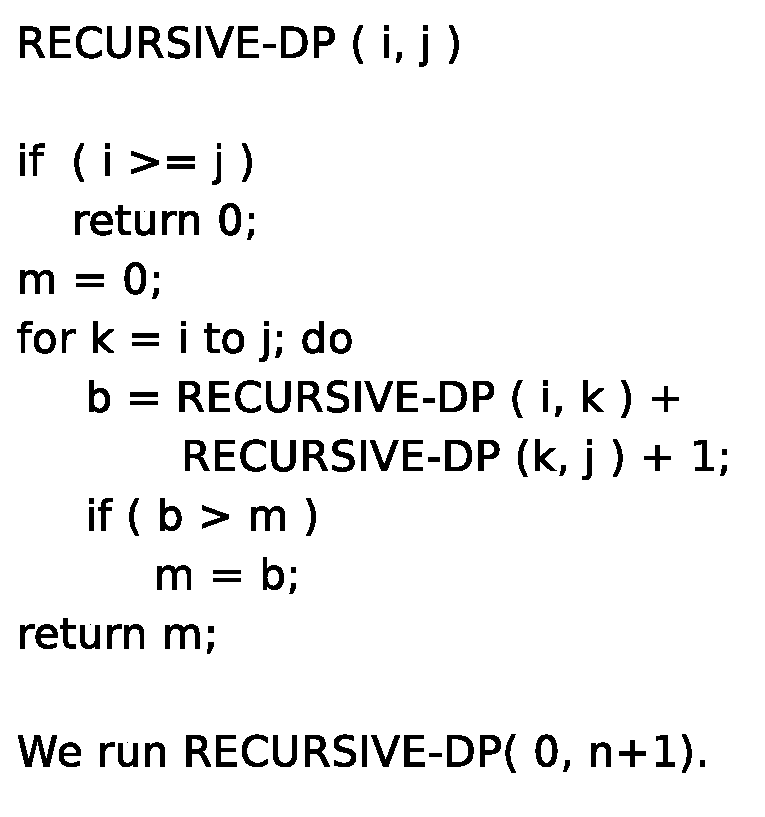
\includegraphics[width=1.0\textwidth]{L7-intervalschedulingdpalgo.eps}%
%      \end{minipage}%
%  \quad
%      \begin{minipage}{0.30\textwidth}
%       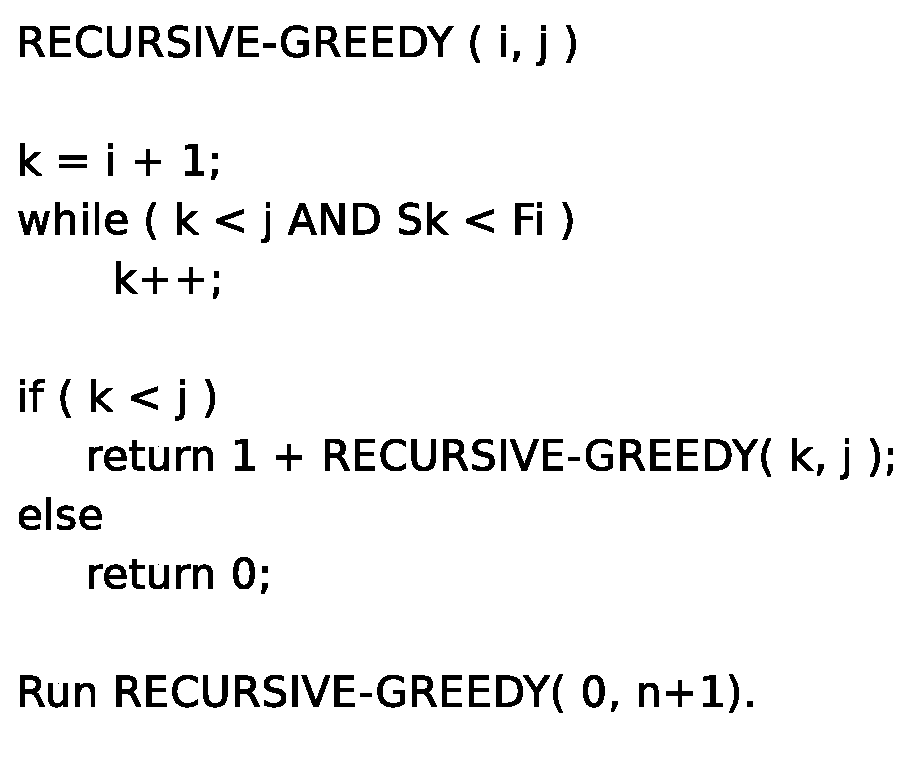
\includegraphics[width=1.0\textwidth]{L7-intervalschedulinggreedyalgo.eps}%
%      \end{minipage}%
%  \quad
%       \begin{minipage}{0.25\textwidth}
%       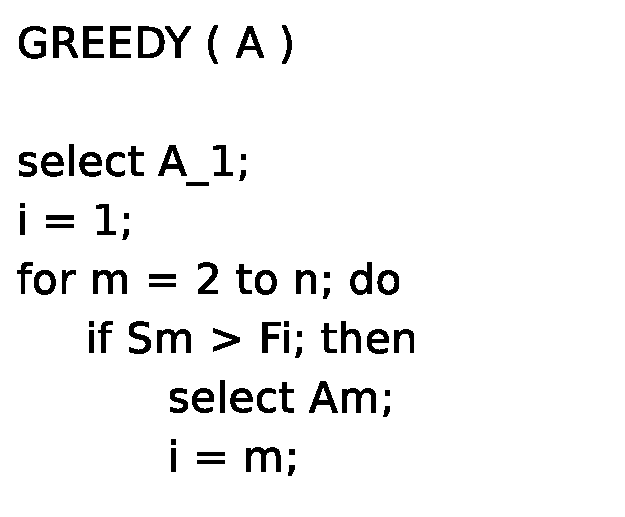
\includegraphics[width=1.0\textwidth]{L7-intervalschedulinggreedyalgo2.eps}%
%      \end{minipage}%
%
%  \end{figure}

\title{CS711008Z  Algorithm Design and Analysis }
\subtitle{ Lecture 8. Algorithm design technique: Linear programming
%\footnote{The slides are made based on Chapter 29 of Introduction to algorithms, Combinatorial optimization algorithm and complexity by C. H. Papadimitriou and K. Steiglitz. } 
}
\author{Dongbo Bu }
\institute{ {\small Institute of Computing Technology \\
Chinese Academy of Sciences, Beijing, China}}

\date{}

\begin{document}
%\begin{CJK}{UTF8}{cyberbit}

\frame{\titlepage}

\frame{
\frametitle{Outline}
\begin{itemize}
\item Some practical problems: {\sc Diet}, {\sc Maximum Flow}, {\sc Minimum Cost Flow}, {\sc MulticommodityFlow}, and {\sc SAT}  problems
\item Linear programming forms:  general form, standard form, and slack form
\item Intuitions of linear program
\item Algorithms: {\sc Simplex} algorithm, {\sc Interior Point} algorithm
\item Smoothed complexity: why simplex algorithm usually takes polynomial time?  
%\item Connection with divide-and-conquer technique;
\end{itemize}
}

\frame{
\begin{block}{}
 Practical problem 1: {\sc Diet} problem \end{block}
}

\frame{
	\frametitle{{\sc Diet} problem} 
	
	\begin{figure}
 
\includegraphics[width=2in] {Stigler.jpg}
\end{figure}
	\begin{itemize} 
	\item In 1945, G. Stigler described the diet problem in the paper  {\it The cost of subsistence}. 
	\item Here we use a simplified version. 
	\end{itemize} 

}

\frame{
\frametitle{{\sc Diet} problem }
A housewife wonders how much money she must spend on foods in order to get all the energy (2000 kcal), protein (55 g), and calcium (800 mg) that she needs every day.

\begin{table}
{ \begin{tabular}{l|ccc|c}\hline
       Food & Energy & Protein & Calcium  & Price \\
 \hline
 Oatmeal & 110 & 4 & 2 & 3 \\
 Whole milk & 160 & 8 & 285 & 9 \\
 Cherry pie & 420 & 4 & 22 & 20 \\
 Pork with beans & 260 & 14 & 80 & 19 \\
\hline
\end{tabular}} {}%
\end{table}

Two solutions:
\begin{itemize}
\item 10 servings of pork with beans: 190 Cents \\
\item  8 servings of milk + 2 servings of pie: 112 Cents.
\end{itemize}
}

\frame{
\frametitle{Linear programming formulation }

A housewife wonders how much money she must spend on foods in order to get all the energy (2000 kcal), protein (55 g), and calcium (800 mg) that she needs every day.

\begin{table}
{ \begin{tabular}{l|ccc|c|c}\hline
       Food & Energy & Protein & Calcium  & Price & \textcolor{red}{Quantity}\\
 \hline
 Oatmeal & 110 & 4 & 2 & 3 & \textcolor{red}{$x_1$}\\
 Whole milk & 160 & 8 & 285 & 9 & \textcolor{red}{$x_2$}\\
 Cherry pie & 420 & 4 & 22 & 20 & \textcolor{red}{$x_3$}\\
 Pork beans & 260 & 14 & 80 & 19 & \textcolor{red}{$x_4$}\\
\hline
     \end{tabular}} {}%
 \end{table}
 \pause
Formalization:
\[
\begin{array}{rrrrrrrrlr}
 \min & 3x_1   &+& 9 x_2   &+& 20x_3   &+& 19x_4   & & \text{money}\\
 s.t. & 110x_1 &+& 160 x_2 &+& 420 x_3 &+& 260 x_4 & \geq 2000 & \text{energy} \\
      & 4 x_1  &+& 8 x_2   &+& 4 x_3   &+& 14 x_4  & \geq 55 & \text{protein}\\
      &  2 x_1 &+& 285 x_2 &+& 22 x_3  &+& 80 x_4  & \geq 800 & \text{calcium}\\
      & x_1    &,& x_2     &,& x_3     &,&    x_4  & \geq 0 \\ 		
\end{array} \nonumber
\]
}

\frame{
\begin{block}{}
 Practical problem 2: {\sc Maximum Flow}
\end{block}
}

\frame{
\frametitle{{\sc Maximum Flow} problem }

\begin{block}{}
{\bf INPUT: }  \\
  A directed graph $G=<V, E>$. Each edge $e=(u, v)$ is associated with a capacity $C(u, v)$. Two special points: \textit{source} $s$ and \textit{sink}  $t$;  \\
{\bf OUTPUT: } \\
  For each edge $e=(u, v)$, to assign a flow $0 \leq f(u, v) \leq C(u, v)$ such that $\sum_{u, (s,u)\in E} f(u, v)$ is maximized. \\
  
 \end{block}
  {\sc Flow conservation} restrictions: at each node (except for $s$ and $t$), the sum of input equals the sum of output.


\begin{figure}
 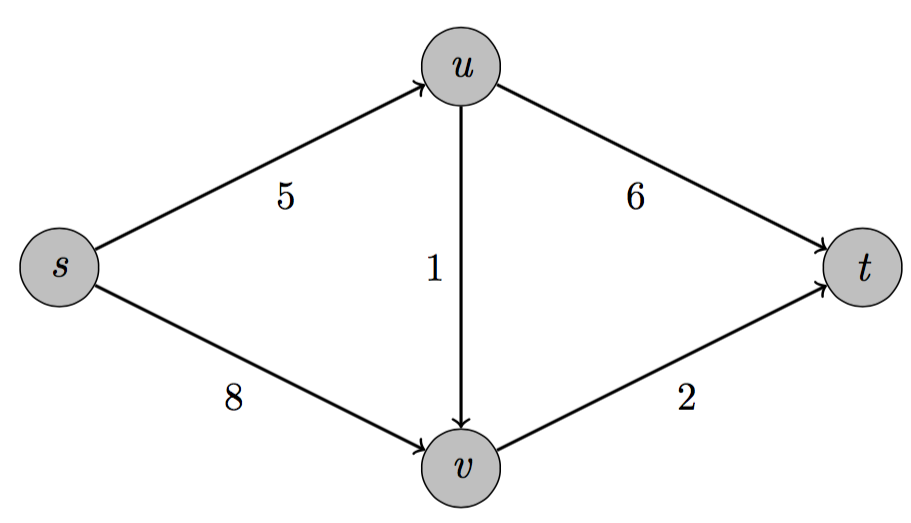
\includegraphics[width=2in] {L8-networkflowexample.png}
\end{figure}
}


\frame{
\frametitle{Linear programming formulation }

\begin{figure}
 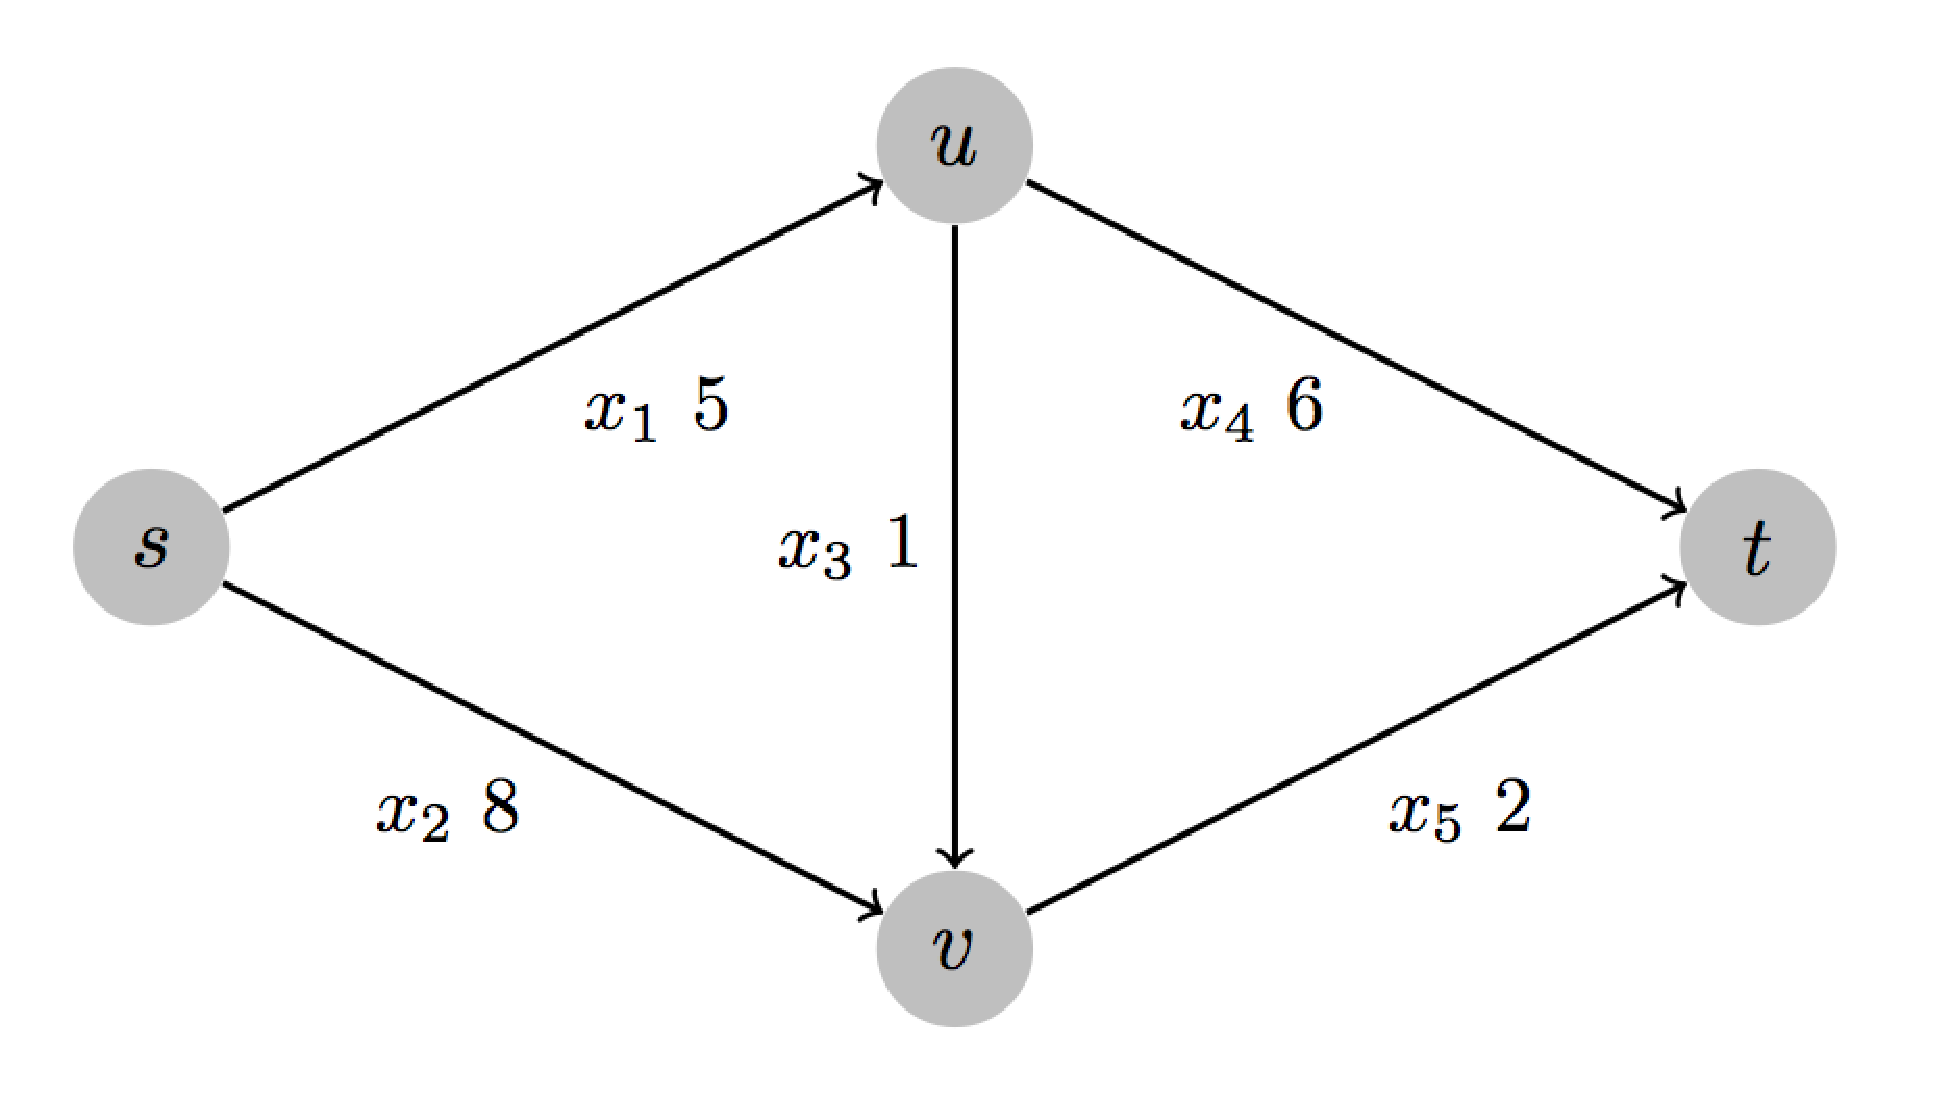
\includegraphics[width=2in] {L8-networkflowexampleLP.eps}
\end{figure}
LP Formulation:
\[
\begin{array}{rrrrrrrrrrlr}
 \max & x_1 &+&  x_2 & &     & &     & &       & & \text{output from  } s\\
 s.t. & x_1 & &      &-& x_3 &-& x_4 & &       & = 0 & \text{node } u \\
      &     & &  x_2 &+& x_3 & &     &-&  x_5  & = 0 & \text{node } v  \\
      &     & &      & &     & &  5   &\geq &  x_1  &\geq 0 & \text{edge }  (s, u)\\
%       &     & &      & &     & &     & &  x_1  &\leq 5 &(node u)\\
      &     & &      & &     & &     & &  ...  & ... & \\
\end{array} \nonumber
\]
}


\frame{
\begin{block}{}
 Practical problem 3: {\sc Minimum Cost Flow} problem
\end{block}
}


\frame{
\frametitle{{\sc Minimum Cost Flow} problem }

\begin{block}{}
\begin{small}
{\bf INPUT: }  \\
  A directed graph $G=<V, E>$. Each edge $e=(u, v)$ is associated with a capacity $C(u, v)$, and a cost $a(u, v)$. If we send $f(u,v)$ units of flow via edge $(u,v)$, we incur a cost of $a(u,v) f(u,v)$. We are also given a flow target $d$. Two special points: \textit{source} $s$ and \textit{sink}  $t$;  \\
{\bf OUTPUT: } \\
  For each edge $e=(u, v)$, to assign a flow $0 \leq f(u, v) \leq C(u, v)$ such that: 
  \begin{enumerate}
  \item We wish to send $d$ units of flow from $s$ to $t$; 
  \item The total cost $\sum_{(u, v) \in E} a(u, v)  f(u, v)$ is minimized. \\

  \end{enumerate}
%  {\sc Flow conservation} requirements: at each node (except for $s$ and $t$), the sum of input equals the sum of output.
\end{small}
\end{block}

% \begin{figure}%
%   \begin{center}%
%     \begin{minipage}{0.4\textwidth}%
%      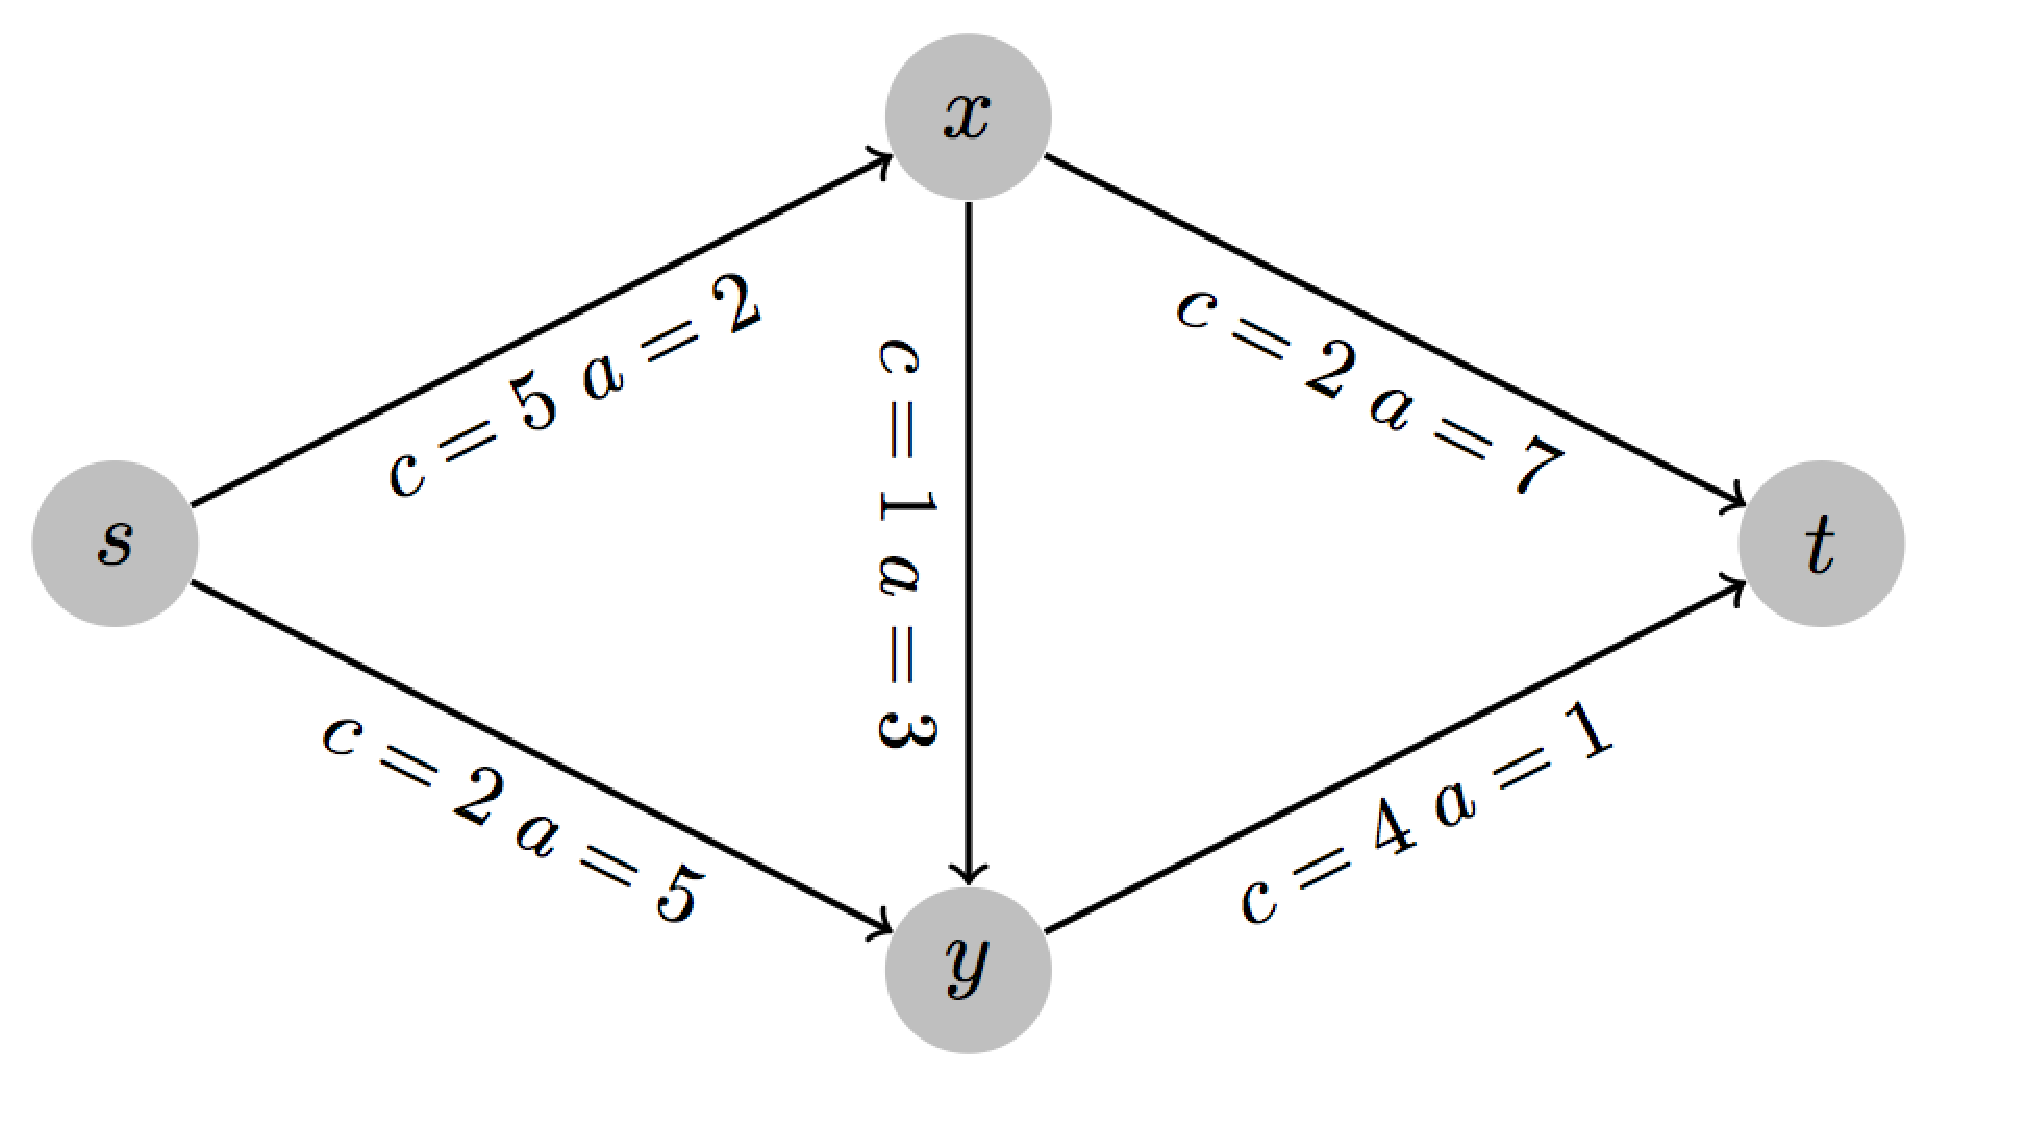
\includegraphics[width=1.0\textwidth]{L8-LPminimumcostflow1.eps}%
%     \end{minipage}%
%     \quad
%     \begin{minipage}{0.4\textwidth}
%      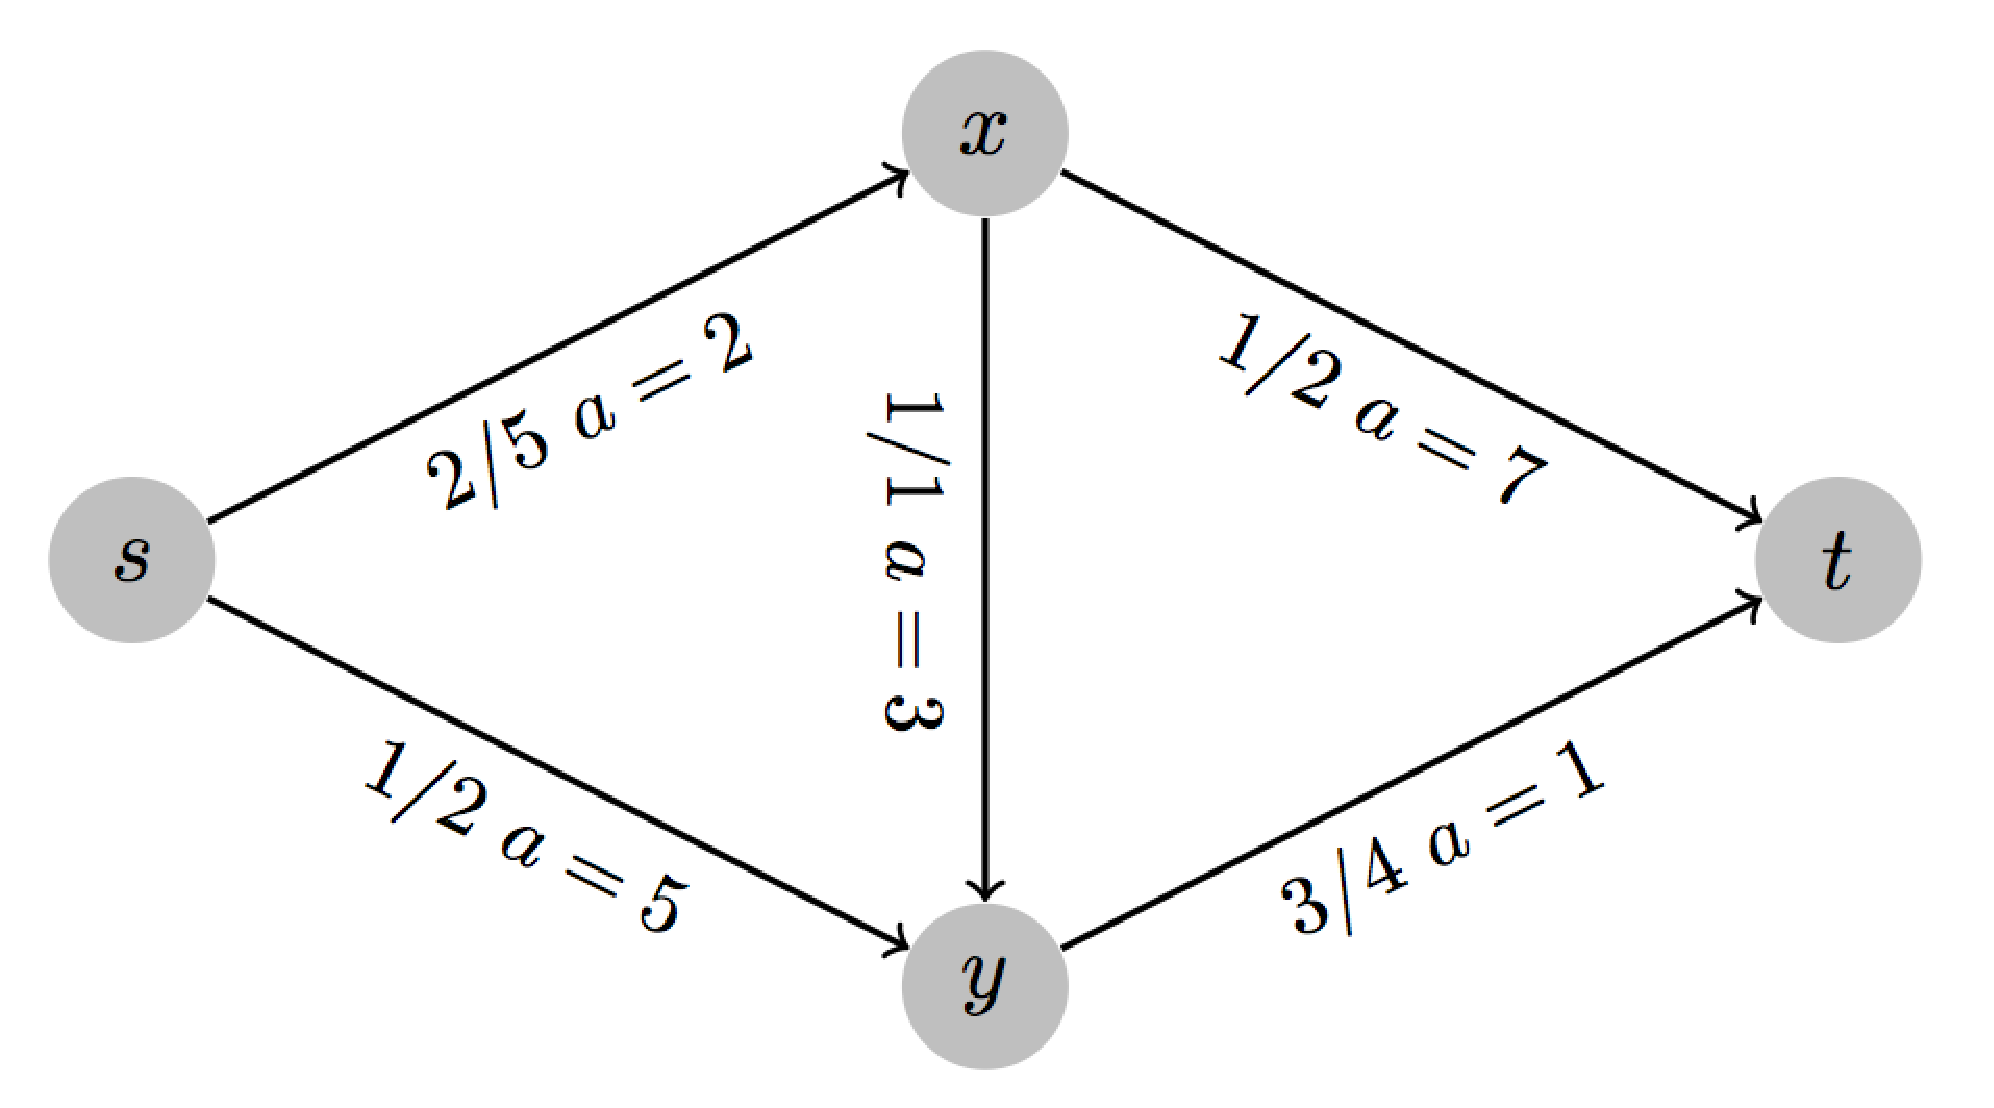
\includegraphics[width=1.0\textwidth]{L8-LPminimumcostflow2.eps}%
%     \end{minipage}%
%     \caption{Cost=$2\times 2 + 1\times 7 + 1\times 3 + 1\times 5 + 3\times 1 = 18$ }
%   \end{center}
% \end{figure}

}


\frame{
\frametitle{Linear programming formulation }

\begin{figure}
 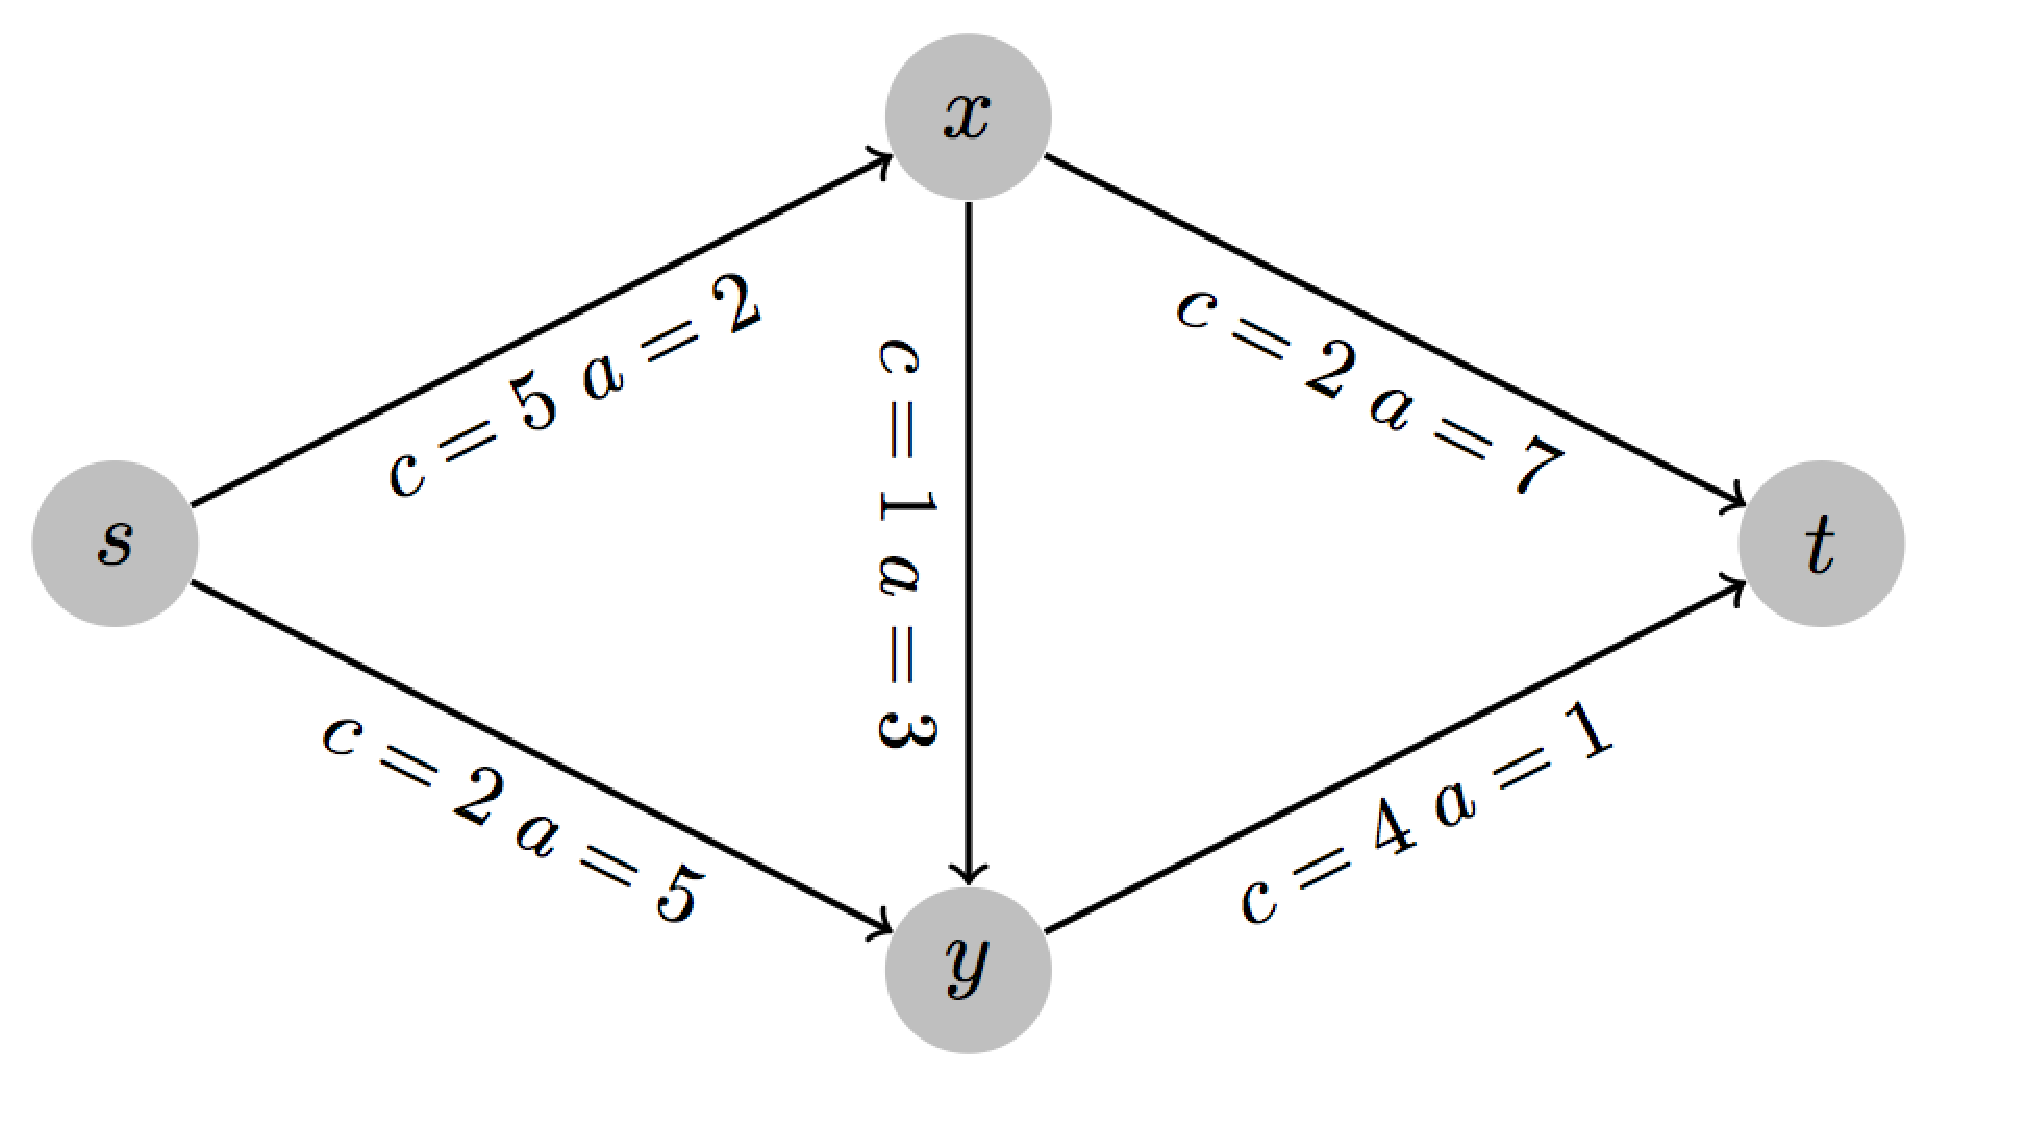
\includegraphics[width=2in] {L8-LPminimumcostflow1.eps}
\end{figure}
LP Formulation:
\[
\begin{array}{rrrrl}
 \min & \sum_{(u, v) \in E} a(u,v)  f(u, v)   & & & \\
 s.t. & f(u,v)   & \leq & C(u,v) & \text{for each } (u,v) \in E\\
      & f(u,v)                & \geq & 0 &  \text{for each }  (u, v) \in E\\
      & \sum_{u, (u, v) \in E} f (u,v) & = & \sum_{w, (v, w) \in E} f (v,w)  & \text{for each }  v\in V-\{s, t\}\\
%       &                         &   &   & u\in V-\{s_i, t_i\} \\
      & \sum_{v, (s, v) \in E} f( s, v) &=& d &  \\
\end{array} \nonumber
\]
}




\frame{
\begin{block}{}
 Practical problem 4: {\sc MultiCommodityFlow} problem
\end{block}
}


\frame{
\frametitle{{\sc MultiCommodityFlow} problem }

\begin{block}{}
{\bf INPUT: }  \\
  A directed graph $G=<V, E>$. Each edge $e$ has a capacity $C_e$. A total of $k$ commodities, and for commodity $i$,  $s_i$, $t_i$, and $d_i$ denote the source, sink, and demand, respectively. \\
{\bf OUTPUT: } \\
  A feasible flow for commodity $i$ (denoted as $f_i$) satisfying the {\sc  flow-conservation}, and {\sc capacity constraints}, i.e.  the aggregate flow on edge $e$ cannot exceed its capacity $C_e$.
\end{block}

\begin{figure}
 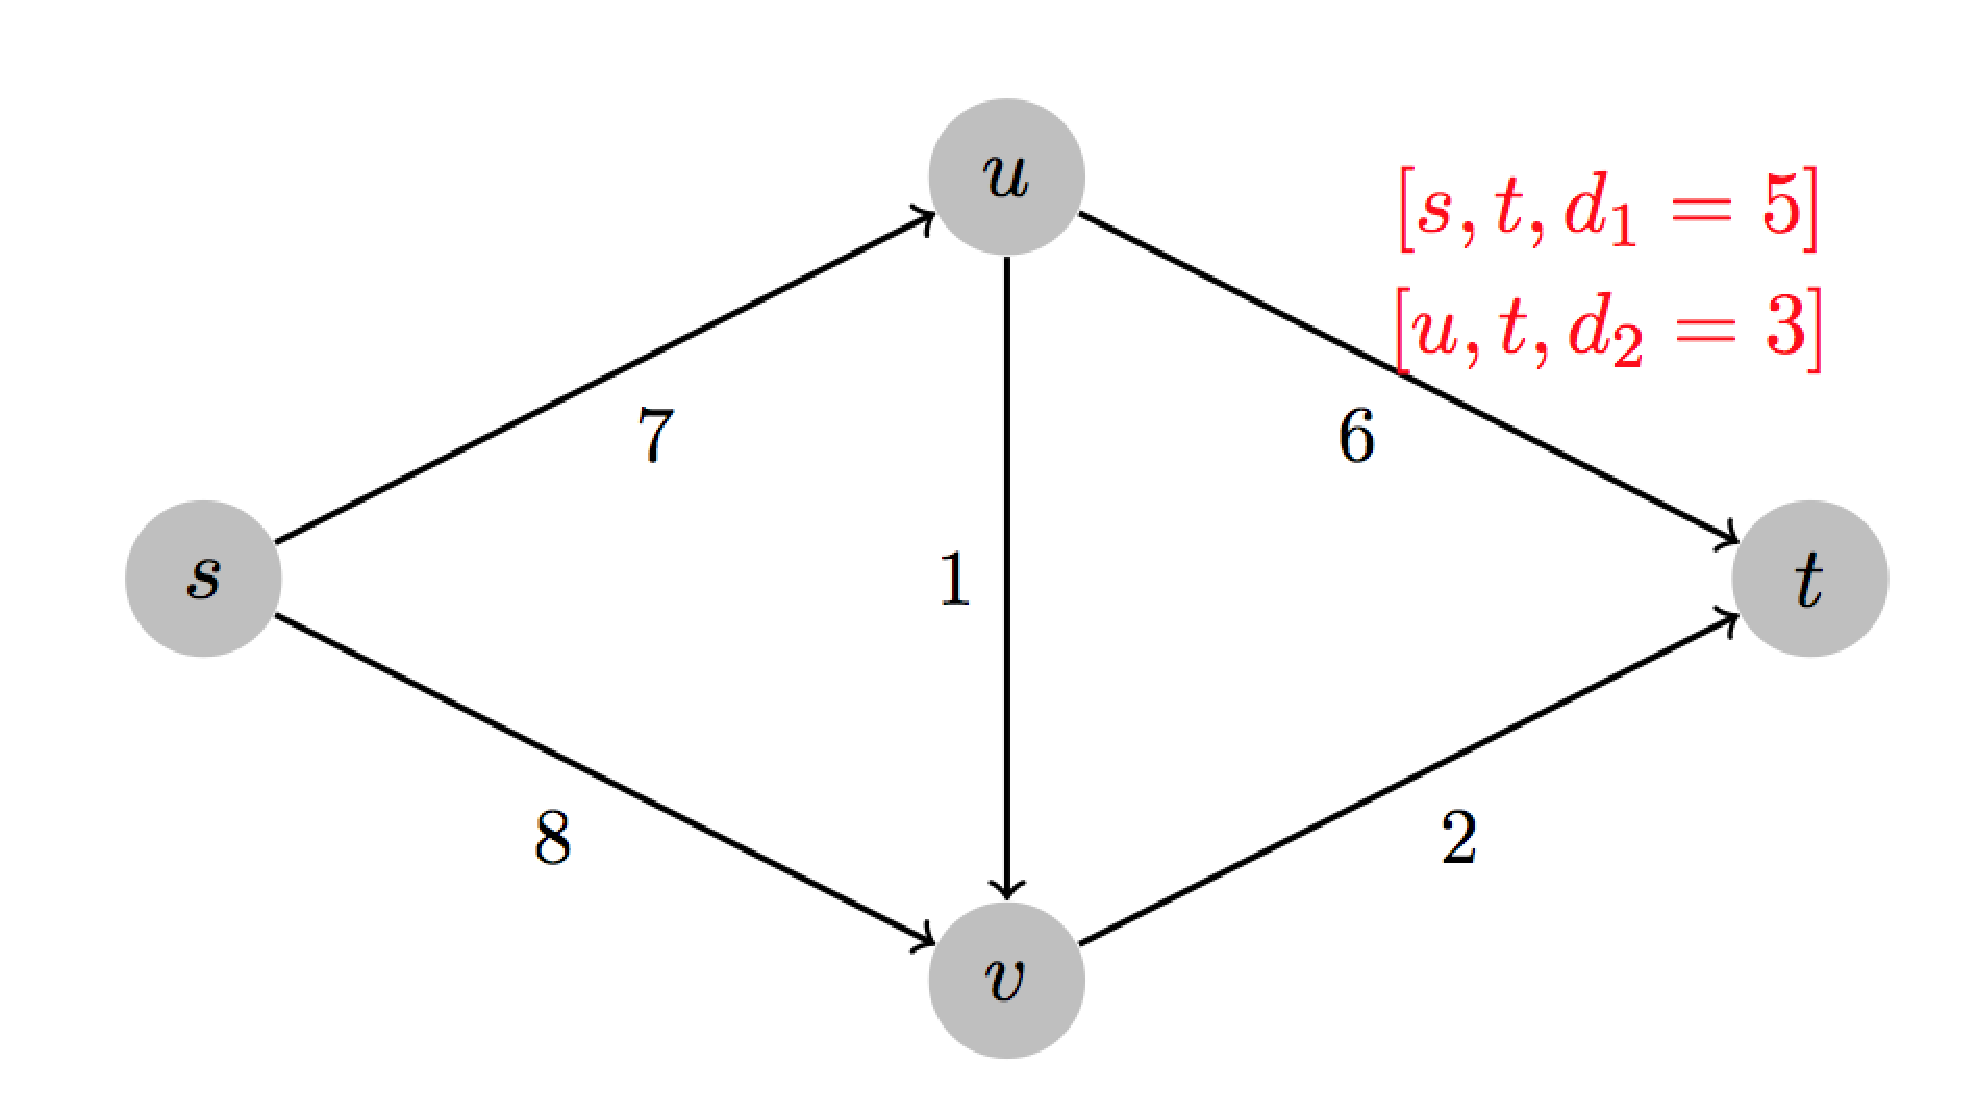
\includegraphics[width=2in] {L8-multicommodityflowexample.eps}
\end{figure}
}



\frame{
\frametitle{Linear programming formulation }

\begin{figure}
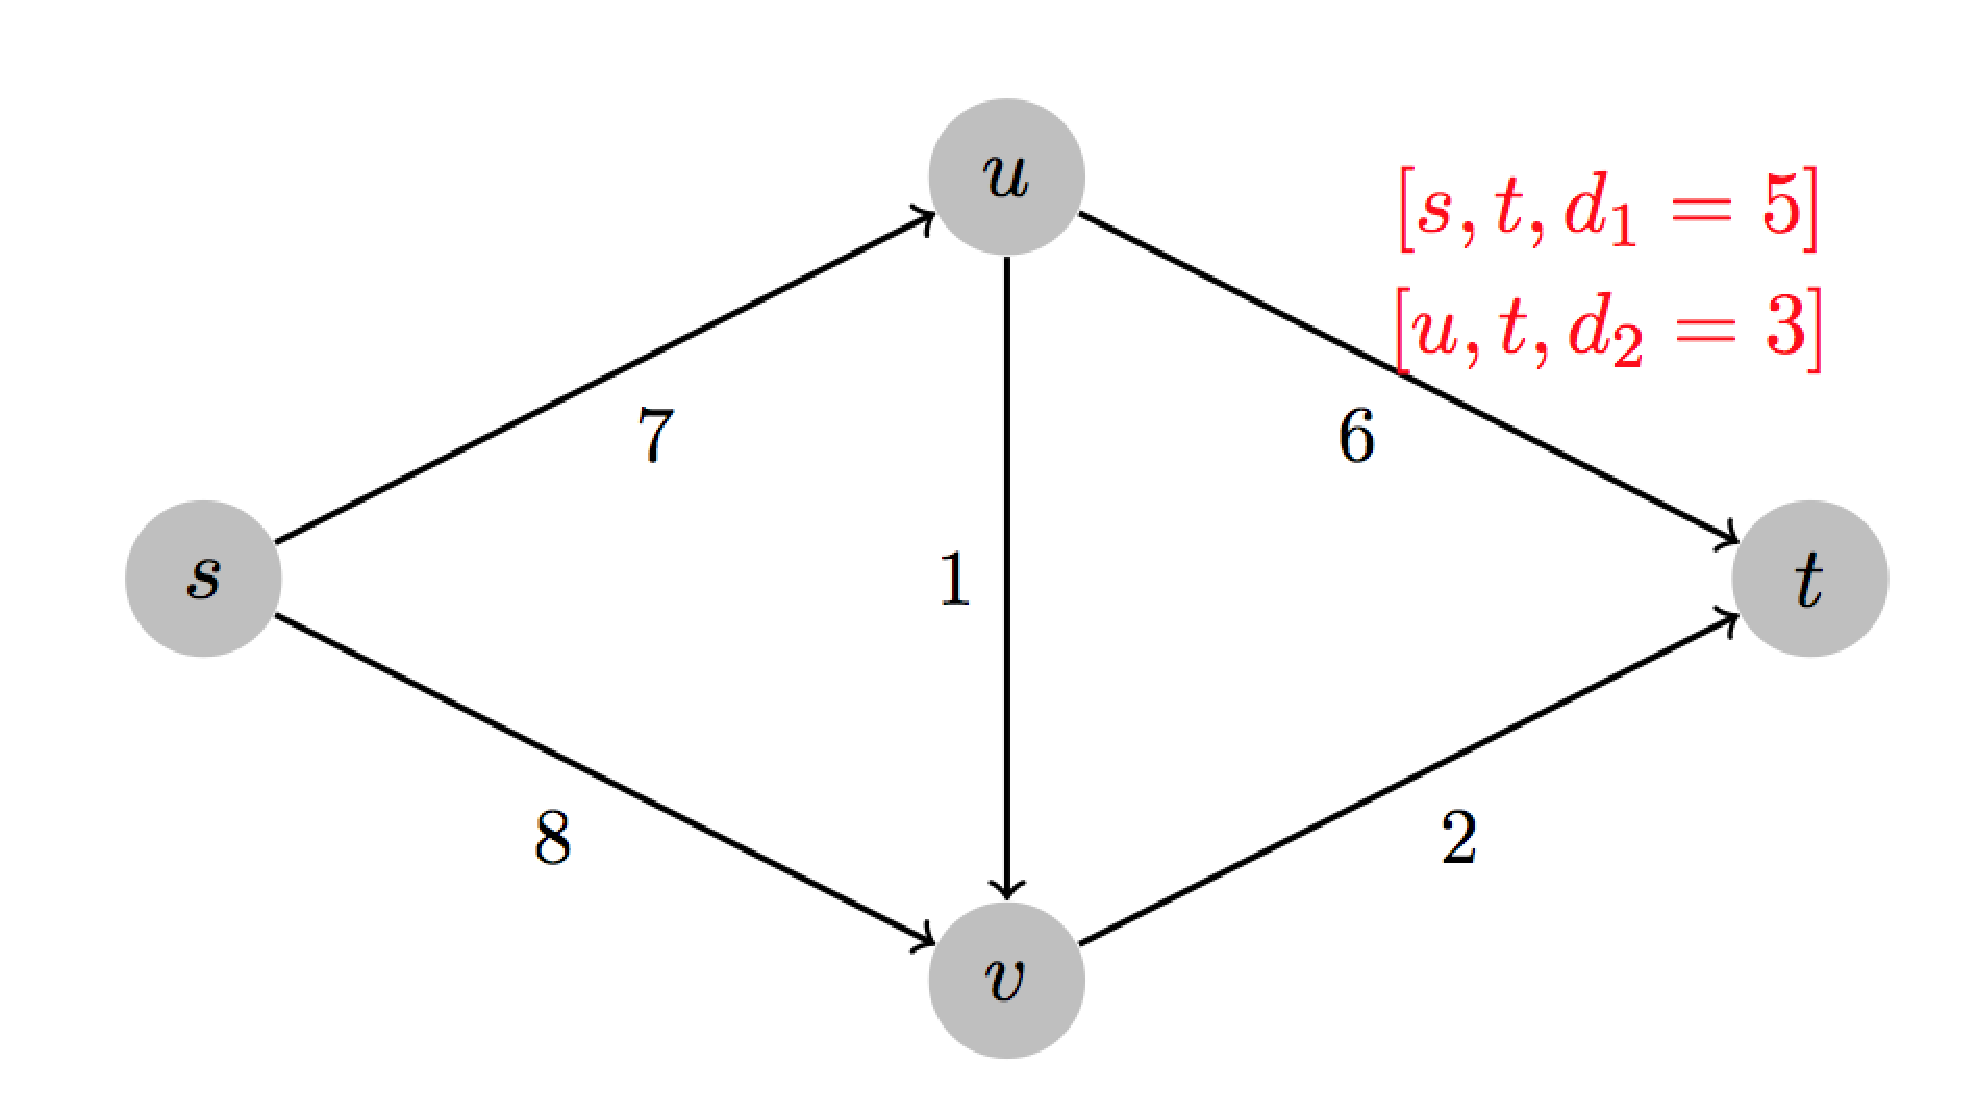
\includegraphics[width=1.7in] {L8-multicommodityflowexample.eps}
\end{figure}
LP Formulation:
\[
\begin{array}{rrrrl}
 \max & 0   & & & \\
 s.t. & \sum_{i=1}^k f_i(u,v)   & \leq & c(u,v) & \text{for each } (u,v) \\
      & f_i(u,v)                & \geq & 0 &  \text{for each }  i, (u, v) \\
      & \sum_{u, (u, v) \in E} f_i (u,v) & = & \sum_{w, (v, w) \in E} f_i (v,w)  & \text{for each } i, v\in V-\{s_i, t_i\} \\
%       &                         &   &   & u\in V-\{s_i, t_i\} \\
      & \sum_{v, (s_i, v) \in E} f_i( s_{i}, v) &=& d_i & \text{for each }  i\\
\end{array} \nonumber
\]

Notes:
\begin{enumerate}
% \item Here $d_i$ denotes the demand for commodity $i$. 
 \item The unusual objective function \textcolor{red}{``max 0'' } is used to express the idea that it suffices to calculate a feasible solution.
 \item \textcolor{red}{Linear programming is the only known polynomial-time algorithm for this problem.}
\end{enumerate}
}

\frame{
\begin{block}{}
 Practical problem 5: {\sc SAT} problem
\end{block}
}

\frame{
\frametitle{{\sc SAT} problem}
\begin{block}{}
{\bf INPUT: }  \\
  A set of $m$ conjunction normal formula (CNF) clauses over $n$ Boolean variables $x_{1}, x_{2}, ..., x_{n}$ \\
{\bf OUTPUT: } \\
  Whether all clauses can be  satisfied by an {\tt TRUE/FALSE} assignment of the $n$ variables.
\end{block}

\begin{itemize} 
\item 
A {\sc SAT } instance:
\[
\begin{array}{rrrrl}
 \Phi & = & ( x_1 \vee \neg x_2 \vee x_3 ) & \wedge \\
      &  & ( \neg x_1 \vee  x_2 \vee \neg x_3 ) & \wedge \\
      &  & (      x_1 \vee  x_2 \vee \neg x_3 ) & \\
 \end{array} \nonumber
\]
\item 
An assignment to make all clauses {\tt TRUE}:

\[
x_{1}=\texttt{TRUE}, x_{2}=\texttt{TRUE}, x_{3}=\texttt{TRUE}
\]
\end{itemize} 
}


\frame{
\frametitle{Linear programming formulation}


A {\sc SAT } instance:
\[
\begin{array}{rrrrl}
 \Phi & = & ( x_1 \vee \neg x_2 \vee x_3 ) & \wedge \\
      &  & ( \neg x_1 \vee  x_2 \vee \neg x_3 ) & \wedge \\
      &  & (      x_1 \vee  x_2 \vee \neg x_3 ) & \\
 \end{array} \nonumber
\]

LP Formulation:
\[
\begin{array}{rrrrl}
 \max & c_1 +&  c_2 +& c_3 & \\
 s.t. & x_1 +& (1-x_2) +& x_3 & \geq c_1 \\
      & (1-x_1) +&  x_2 +& (1-x_3) & \geq c_2 \\
      & x_1 +&  x_2 +& (1-x_3) & \geq c_3 \\
      & x_1 ,& x_2 ,& x_3 & = 0/1 \\
      & c_1 ,& c_2 ,& c_3 & = 0/1
\end{array} \nonumber
\]

Intuitive idea:
\begin{itemize}
\begin{footnotesize}
\item Constraints: The left-hand side of a constraint represents the number of satisfied literals; thus, a constraint allows $c_i$ to be $1$ if there are at least one satisfied liters. 
\item Objective function:  The objective function denotes the number of satisfied clauses. Thus, $\Phi$ is satisfiable iff $c_1+c_2+c_3=3$.
\end{footnotesize}
\end{itemize}
}

\frame{
	\begin{block}{}
		Genome rearrangement distance problem [M. Shao, 2014]
	\end{block}
}

%\frame
%{
%	\frametitle{Practical problem: genome rearrangement distance}
%	\begin{itemize}
%	\item The minimum number of operations to transform $G_1$ into $G_2$
%	\end{itemize}
%
%	\vspace{0.2cm}
%
%	\begin{center}
%		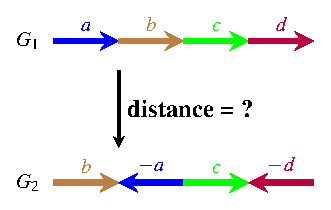
\includegraphics[width=0.6\textwidth]{mingfudistance.eps}
%	\end{center}
%	Operations:  reverse a fragment of the genome; 
%}
%
%\frame
%{
%	\frametitle{Adjacency graph: a more succinct formulation}
%	\begin{center}
%		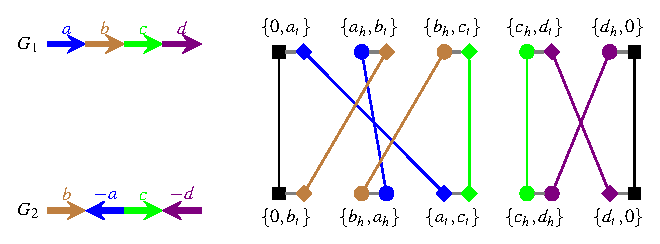
\includegraphics[width=0.95\textwidth]{mingfuadjgraph.eps}
%	\end{center}
%	\begin{itemize}
%	\item<2-> DCJ distance = (\#adjacencies) $-$ (\#cycles).  
%	\item <3-> DCJ distance = 3 in this example. 
%	\item<4-> To minimize DCJ distance, we need to compute a decomposition of the corresponding
%		adjacency graph with maximized number of cycles.
%	\end{itemize}
%}
%
%
%
%
%
%\frame
%{
%	\frametitle{Problem Statement}
%
%	\vspace{-0.3cm}	
%
%	{\bf Problem:} given an undirected graph $G=(V,E)$, to choose $k$ edges and remove others,
%	such that the number of connected components in the remaining graph is maximized. \\
%	({\bf Formulate this problem as an ILP}.)
%
%	\vspace{0.6cm}	
%
%	\begin{center}
%	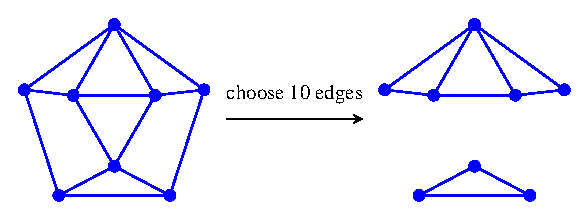
\includegraphics[width=\textwidth]{mingfustar.eps}
%	\end{center}
%}
%
%\frame
%{
%	\frametitle{ILP Formulation}
%
%	Consider the following example with $k = 3$.
%
%	\begin{center}
%	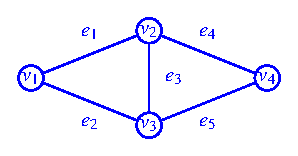
\includegraphics[width=0.5\textwidth]{mingfuexample.eps}
%	\end{center}
%
%	\begin{itemize}
%	\item<2-> For each edge $e_i$, we use a binary variable $x_i$ to indicate whether $e_i$ is chosen.
%		We use the following constraint to guarantee exactly $k$ edges are chosen:
%		\begin{displaymath}
%			x_1 + x_2 + x_3 + x_4 + x_5 = 3
%		\end{displaymath}
%	\end{itemize}
%
%}
%
%\frame
%{
%	\frametitle{ILP Formulation}
%
%	\begin{center}
%	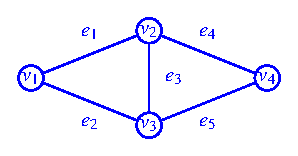
\includegraphics[width=0.5\textwidth]{mingfuexample.eps}
%	\end{center}
%
%
%	\begin{itemize}
%	\item<1-> To count the number of connected components, for vertex $v_j$, $1\le j \le |V|$,
%		we use a variable $y_j$ to indicate the {\bf label} of $v_j$, and set {\bf distinct} upper 
%		bounds for all the labels:
%		\begin{eqnarray*}
%			1\le  y_1  \le 1\\ 
%			1\le  y_2  \le 2\\ 
%			1\le  y_3  \le 3\\ 
%			1\le  y_4  \le 4\\ 
%		\end{eqnarray*}
%	\end{itemize}
%
%}
%
%\frame
%{
%	\frametitle{ILP Formulation}
%
%	\begin{center}
%	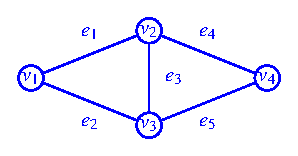
\includegraphics[width=0.5\textwidth]{mingfuexample.eps}
%	\end{center}
%
%	\begin{itemize}
%	\item<1-> We guarantee that if an edge is chosen, then its two adjacent vertices have the same label: 
%		\begin{align*}
%			y_1 \le y_2 + 1 \cdot (1 - x_1);\  y_2 \le y_1 + 2 \cdot (1 - x_1) \tag{for $e_1$}\\
%			y_1 \le y_3 + 1 \cdot (1 - x_2);\  y_3 \le y_1 + 3 \cdot (1 - x_2) \tag{for $e_2$}\\
%			y_2 \le y_3 + 2 \cdot (1 - x_3);\  y_3 \le y_2 + 3 \cdot (1 - x_3) \tag{for $e_3$}\\
%			y_2 \le y_4 + 2 \cdot (1 - x_4);\  y_4 \le y_2 + 4 \cdot (1 - x_4) \tag{for $e_4$}\\
%			y_3 \le y_4 + 3 \cdot (1 - x_5);\  y_4 \le y_3 + 4 \cdot (1 - x_5) \tag{for $e_5$}\\
%		\end{align*}
%	\end{itemize}
%}
%
%\frame
%{
%	\frametitle{ILP Formulation}
%
%	\begin{center}
%	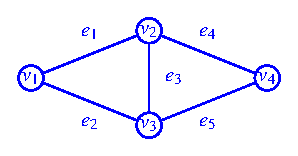
\includegraphics[width=0.5\textwidth]{mingfuexample.eps}
%	\end{center}
%
%	\begin{itemize}
%	\item<2-> The equality can propagate along the chosen edges. Thus, in the remaining graph
%		all vertices in the same connected component have the same label.
%
%	\item<3-> Since all vertices have distinct upper bounds, in each connected
%	component, at most one vertex can reach its upper bound. Thus, we
%	can use the number of vertices whose upper bound is reached, to count the number of connected components.
%
%	\end{itemize}
%}
%
%
%\frame
%{
%	\frametitle{ILP Formulation}
%
%	\begin{center}
%	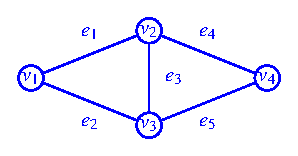
\includegraphics[width=0.5\textwidth]{mingfuexample.eps}
%	\end{center}
%
%	\begin{itemize}
%	\item<2-> We use a binary variable $z_j$ to indicate whether the label of $v_j$ reaches its upper bound:
%		\begin{eqnarray*}
%			1 \cdot z_1 \le y_1 \\
%			2 \cdot z_2 \le y_2 \\
%			3 \cdot z_3 \le y_3 \\
%			4 \cdot z_4 \le y_4 
%		\end{eqnarray*}
%	We can verify that, $z_j = 1$ only if $y_j = j$, i.e., the label of $v_j$ reaches its upper bound.
%	\end{itemize}
%}
%
%
%\frame
%{
%	\frametitle{ILP Formulation}
%
%	\begin{center}
%	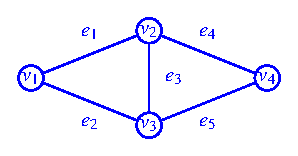
\includegraphics[width=0.5\textwidth]{mingfuexample.eps}
%	\end{center}
%
%	\begin{itemize}
%	\item<2-> The objective function of the ILP formulation can be set to maximize the number of vertices
%		whose upper bound can be reached:
%		\begin{displaymath}
%			\max z_1 + z_2 + z_3 + z_4
%		\end{displaymath}
%	\end{itemize}
%}


\frame
{
	\frametitle{Background: Evolution of Genomes}

	\begin{center}
		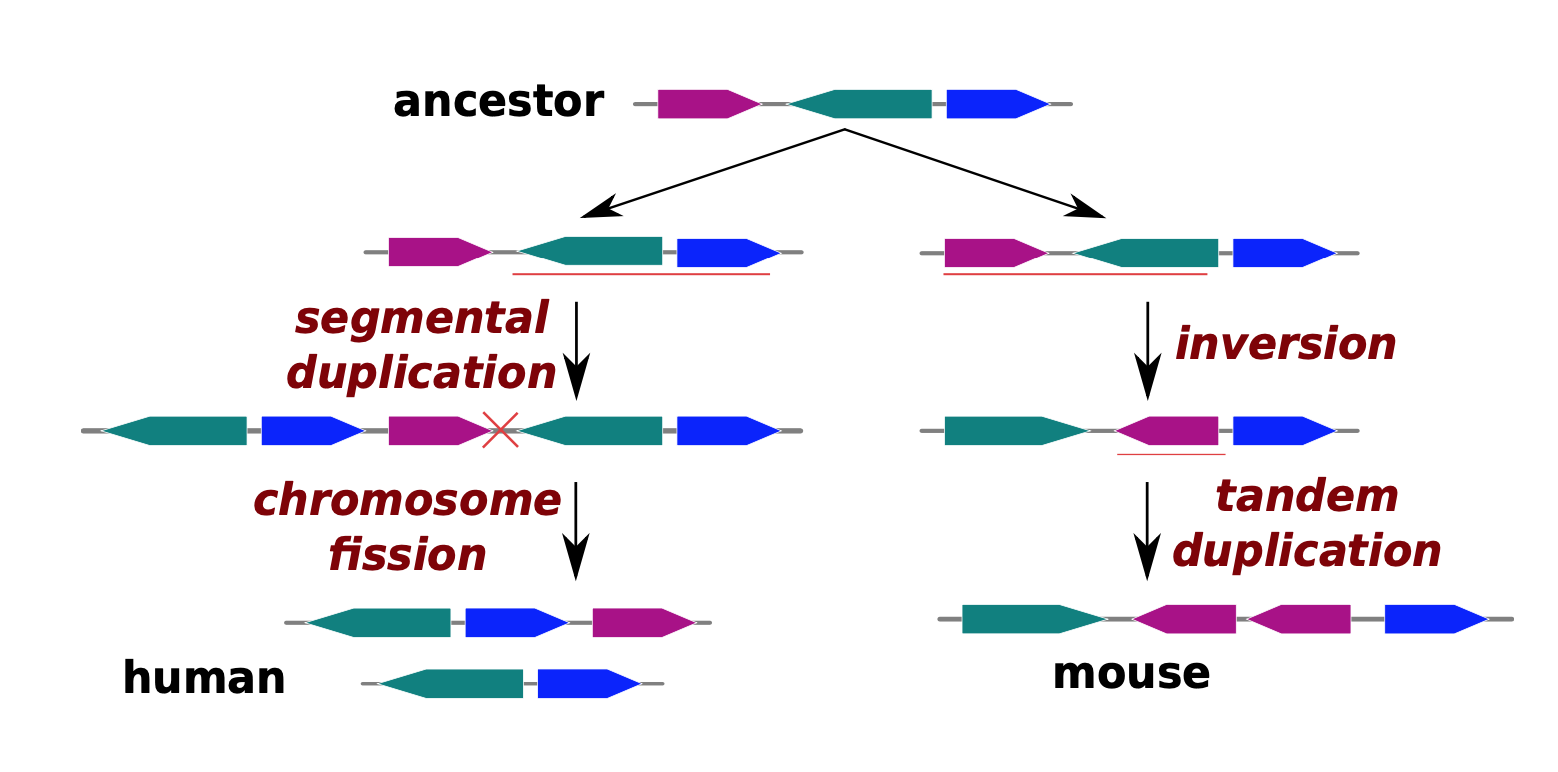
\includegraphics[width=0.85\textwidth]{L8-DCJ1.png}
	\end{center}

	%\vspace{-0.2cm}

	\begin{enumerate}
	\item<1-> {\bf Rearrangements:} inversion, translocation, transposition, chromosome fission and fusion, etc.

	\vspace{0.1cm}

	\item<1-> {\bf Content-modifying events:} segmental duplication, tandem duplication, lateral gene transfer, etc.
	\end{enumerate}

	%\begin{center}
	%\includegraphics[width=0.92\textwidth]{figures/events.pdf}
	%\end{center}
}

\frame
{
	\frametitle{Model of a Genome}
	\vspace{-0.4cm}
	\begin{itemize}
	\item {\bf Genome:} a set of chromosomes
	\item {\bf Chromosome:} a linear/circular list of genes~(synteny blocks)
	\end{itemize}

	\begin{center}
		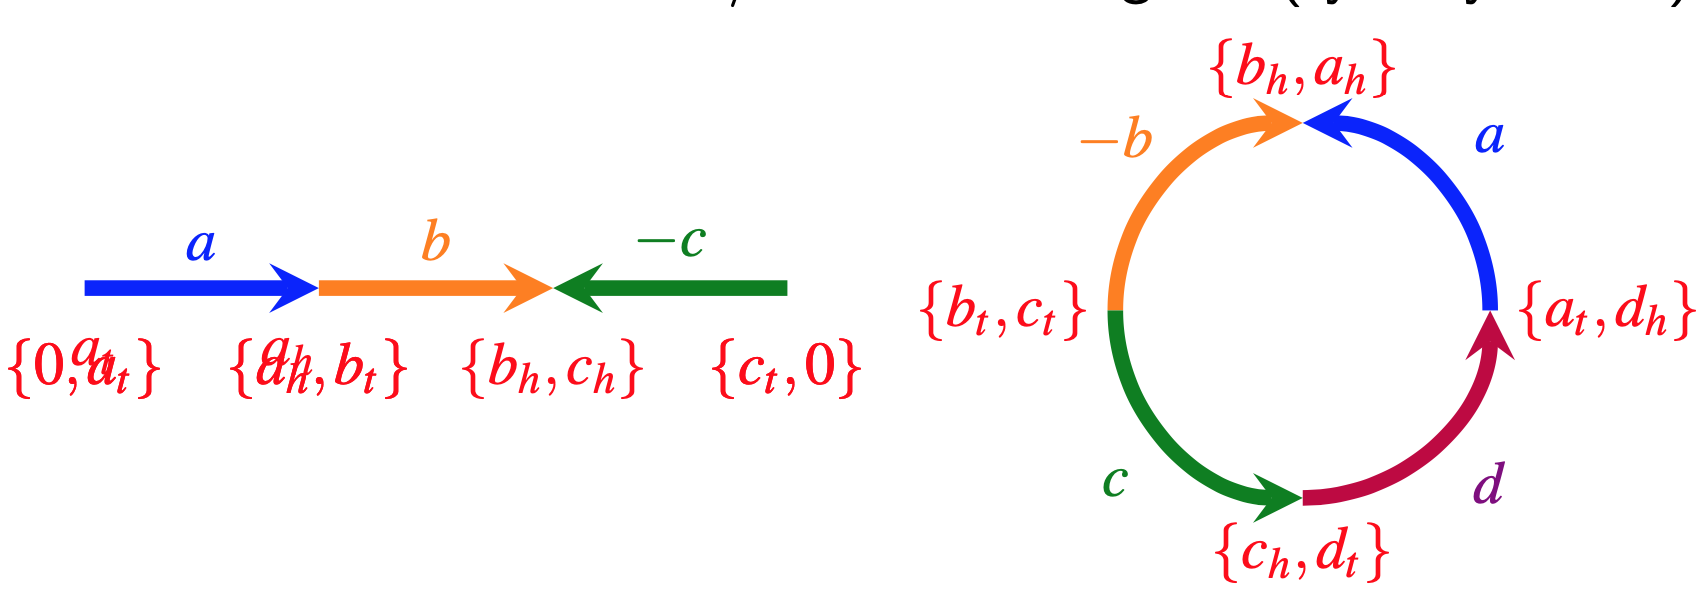
\includegraphics[width=0.7\textwidth]{L8-DCJ2.png}
	\end{center}

	\begin{itemize}
	\item<1-> {\bf Extremities:} two ends~({\bf head} and {\bf tail}) of a gene
	\item<1-> {\bf Adjacency:} two consecutive extremities
	\item<1-> {\bf Null extremity:} special extremity $0$ added to each end of\\ the linear chromosomes
	\end{itemize}
}

\frame
{
	\frametitle{Double-Cut-and-Join~(DCJ) Operation}
	\begin{itemize}
	\item {\bf Input:} two adjacencies
	\item {\bf Output:} two new adjacencies created by recombining the four involved extremities
	\item {DCJ operation can model most of the genome rearrangement events (but not content-modifying events).}
	\end{itemize}

	\begin{center}
		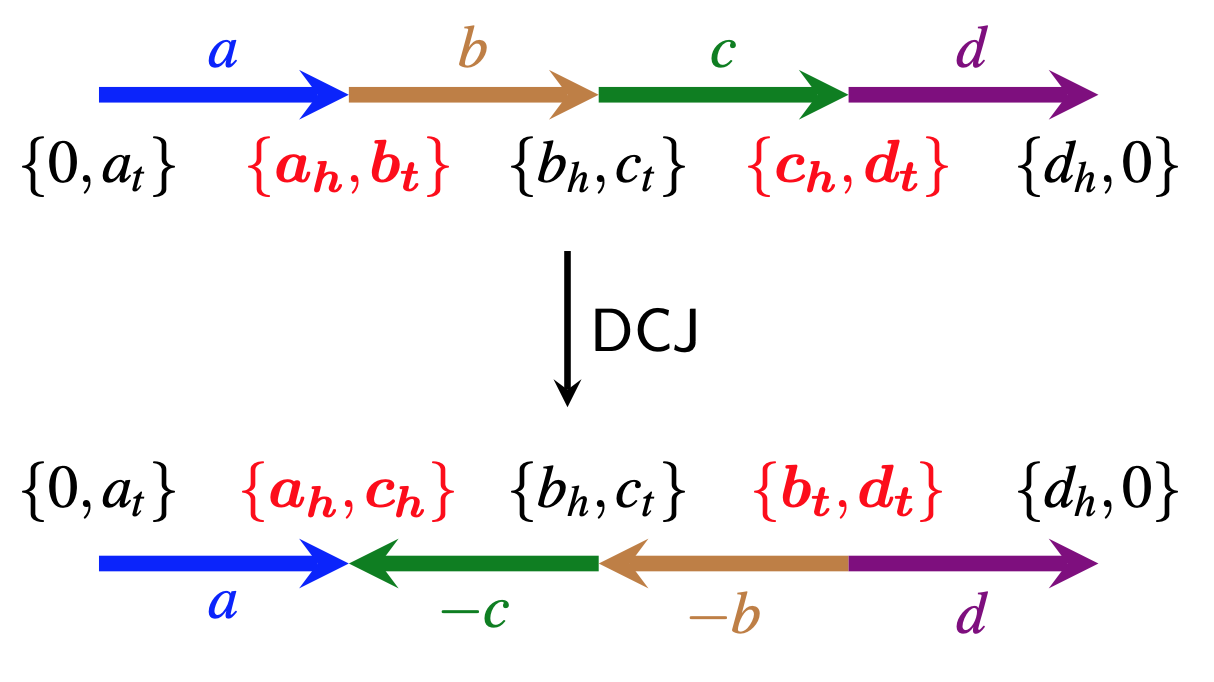
\includegraphics[width=0.7\textwidth]{L8-DCJ3.png}
	\end{center}

}

\frame
{
	\frametitle{DCJ Distance}
	\vspace{-0.6cm}
	\begin{itemize}
	\item The minimum number of DCJ operations to transform $G_1$ into $G_2$
	\end{itemize}

	\begin{center}
		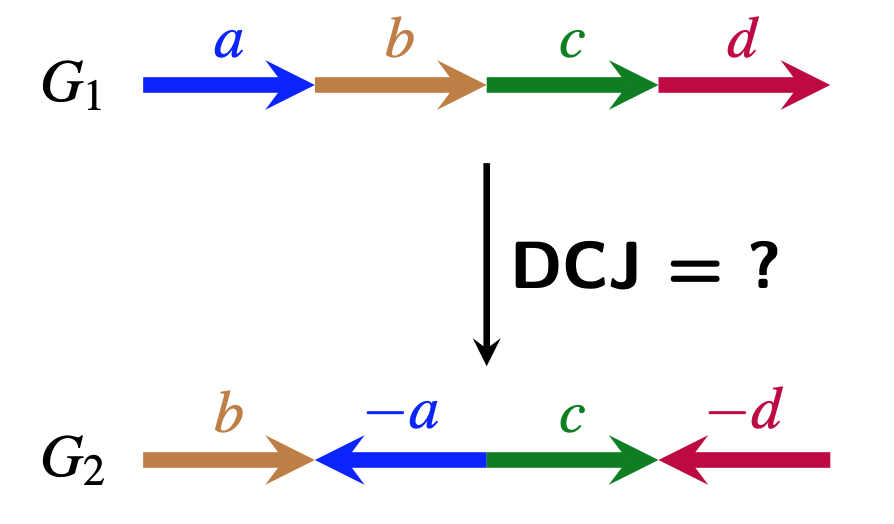
\includegraphics[width=0.7\textwidth]{L8-DCJ4.png}
	\end{center}

	\begin{itemize}
	\item<1-> For two genomes {\bf without duplicate genes}, the DCJ distance can 
		be computed in {\bf linear time}~({\it Yancopoulos et al., 2005, Bergeron et al., 2006}).
	\end{itemize}
}

\frame
{
	\frametitle{Adjacency Graph}

	\begin{center}
		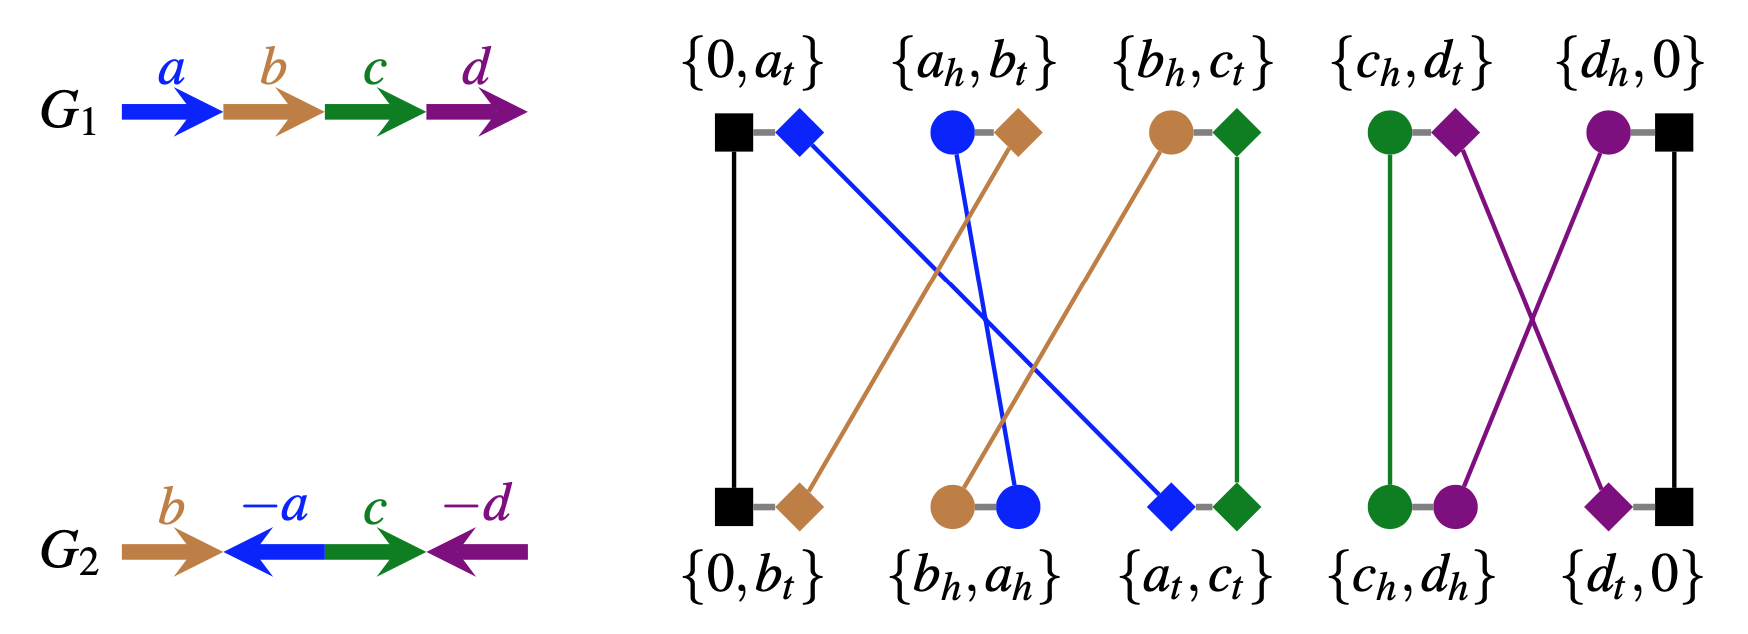
\includegraphics[width=0.7\textwidth]{L8-DCJ5.png}
	\end{center}

	\begin{itemize}
	\item<1-> The adjacency graph consists of vertex-disjoint cycles, when the
		given two genomes don't contain duplicated genes.
	\item<1-> DCJ distance = (\#adjacencies) $-$ (\#cycles). (\small Proof can be found at:
			A., Bergeron, J. Mixtacki, and J. Stoye. "A unifying view of genome rearrangements.", 2006)
	\item<1-> In this example, DCJ distance = 5 - 2 = 3.

	\end{itemize}
}

\frame
{
	\frametitle{\fontsize{0.483cm}{1em}\selectfont DCJ Distance for Genomes with Duplicate Genes}

	\begin{itemize}

	\item<1-> Real genomes usually contain many genes with multiple copies~(i.e., homologous genes).
	\vspace{0.1cm}

	\item<1-> Different one-to-one correspondence between homologous genes lead to different
		DCJ distance (see next slide).

	\item<1-> We assume the gene copy number for each gene is the same, as DCJ operation does not modify gene-content.


	\item<1-> {\bf Problem:} find a one-to-one correspondence between duplicate genes, 
		such that the number of cycles induced by this one-to-one correspondence is maximized
	\item<1-> This problem is NP-hard.
	\item<1-> {Previous work:} 
		\begin{itemize}
		\item {Heuristics:} ({\it Chen et al., 2005, Suksawatchon et al., 2007})
		\item {Approximations:} ({\it Marron et al., 2003, Shao et al., 2012})
		\end{itemize}

	\item<1-> An ILP formulation for this problem~(Shao et al., 2014).
	\end{itemize}
}

\frame
{
	\frametitle{Genomes with Duplicate Genes}

	\begin{center}
		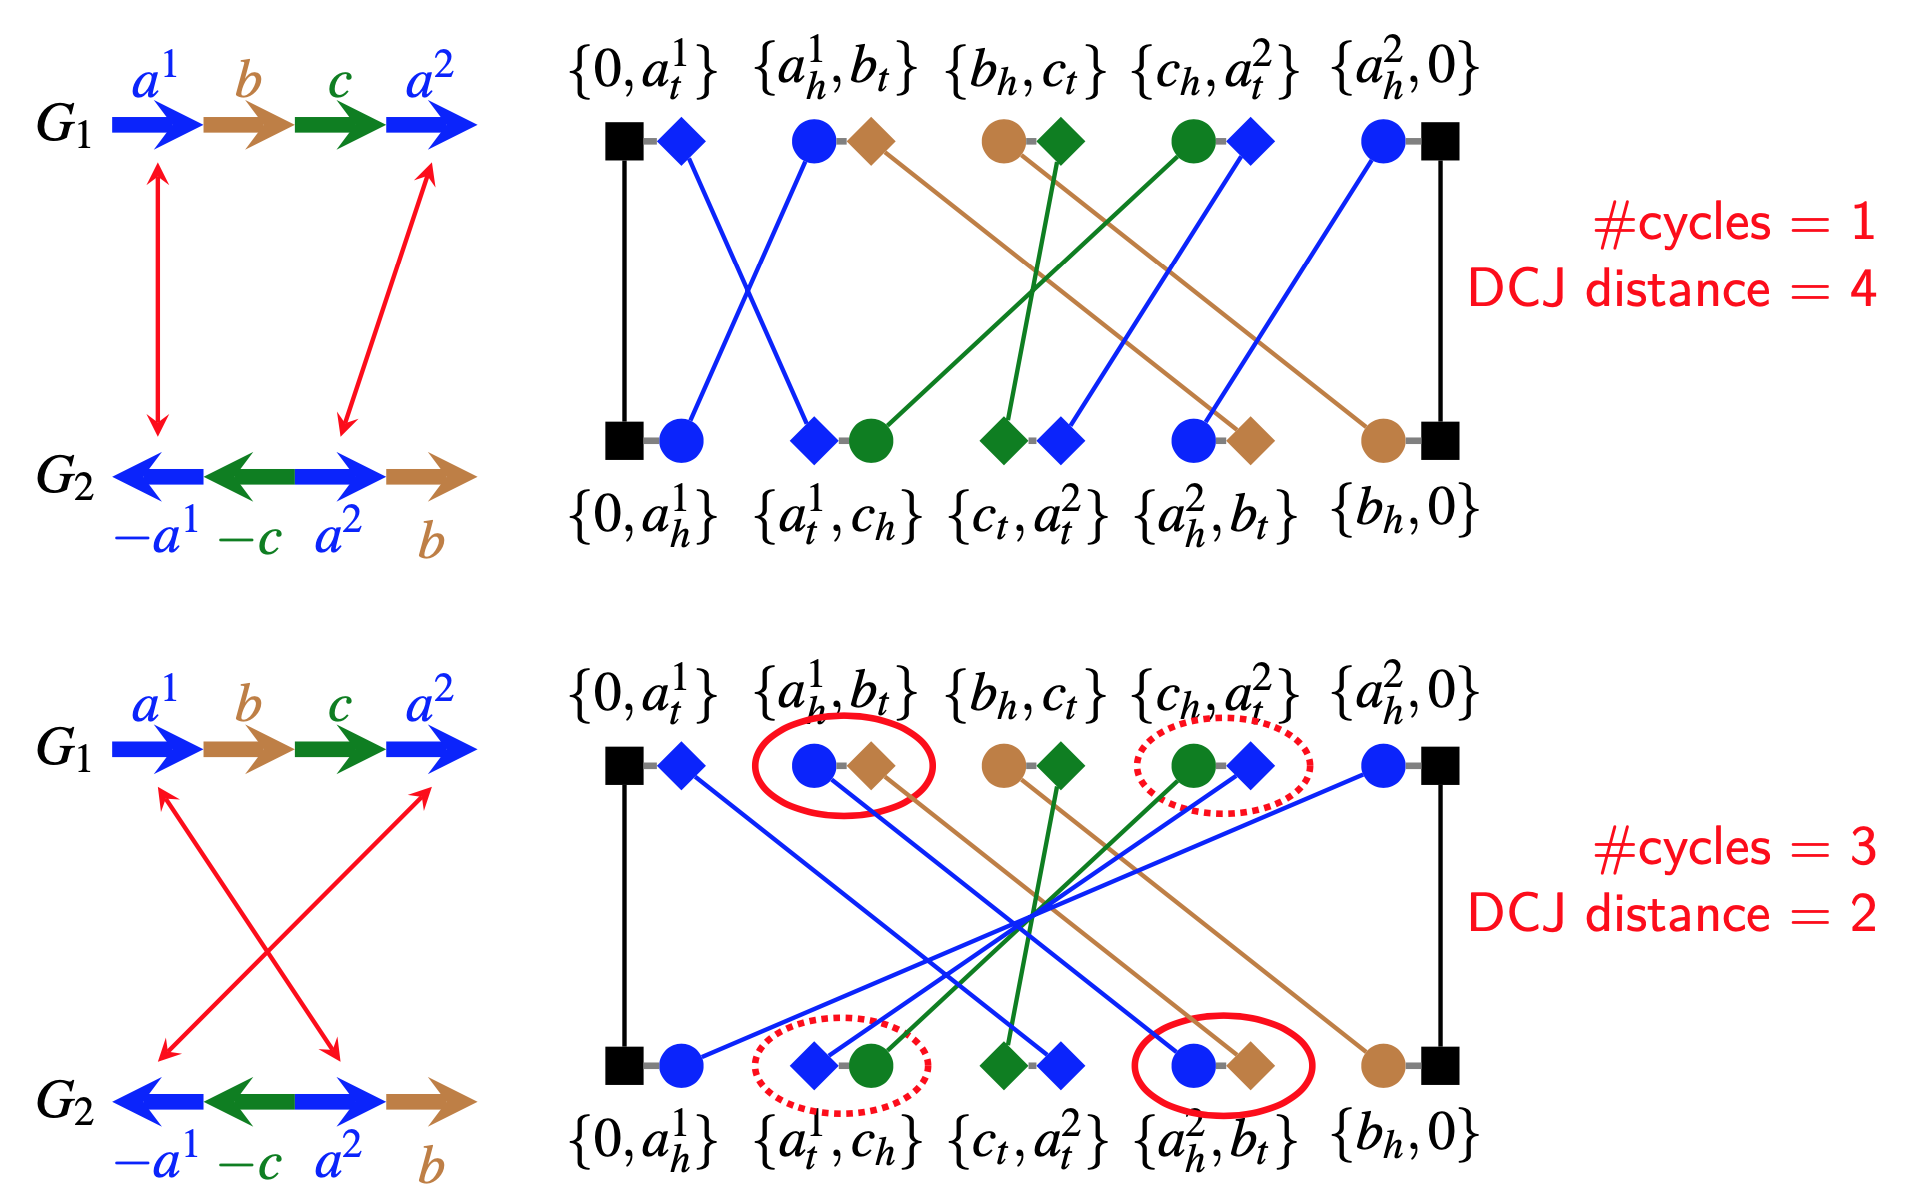
\includegraphics[width=0.7\textwidth]{L8-DCJ6.png}
	\end{center}

}

\frame
{
	\frametitle{ILP Formulation}

	\begin{center}
		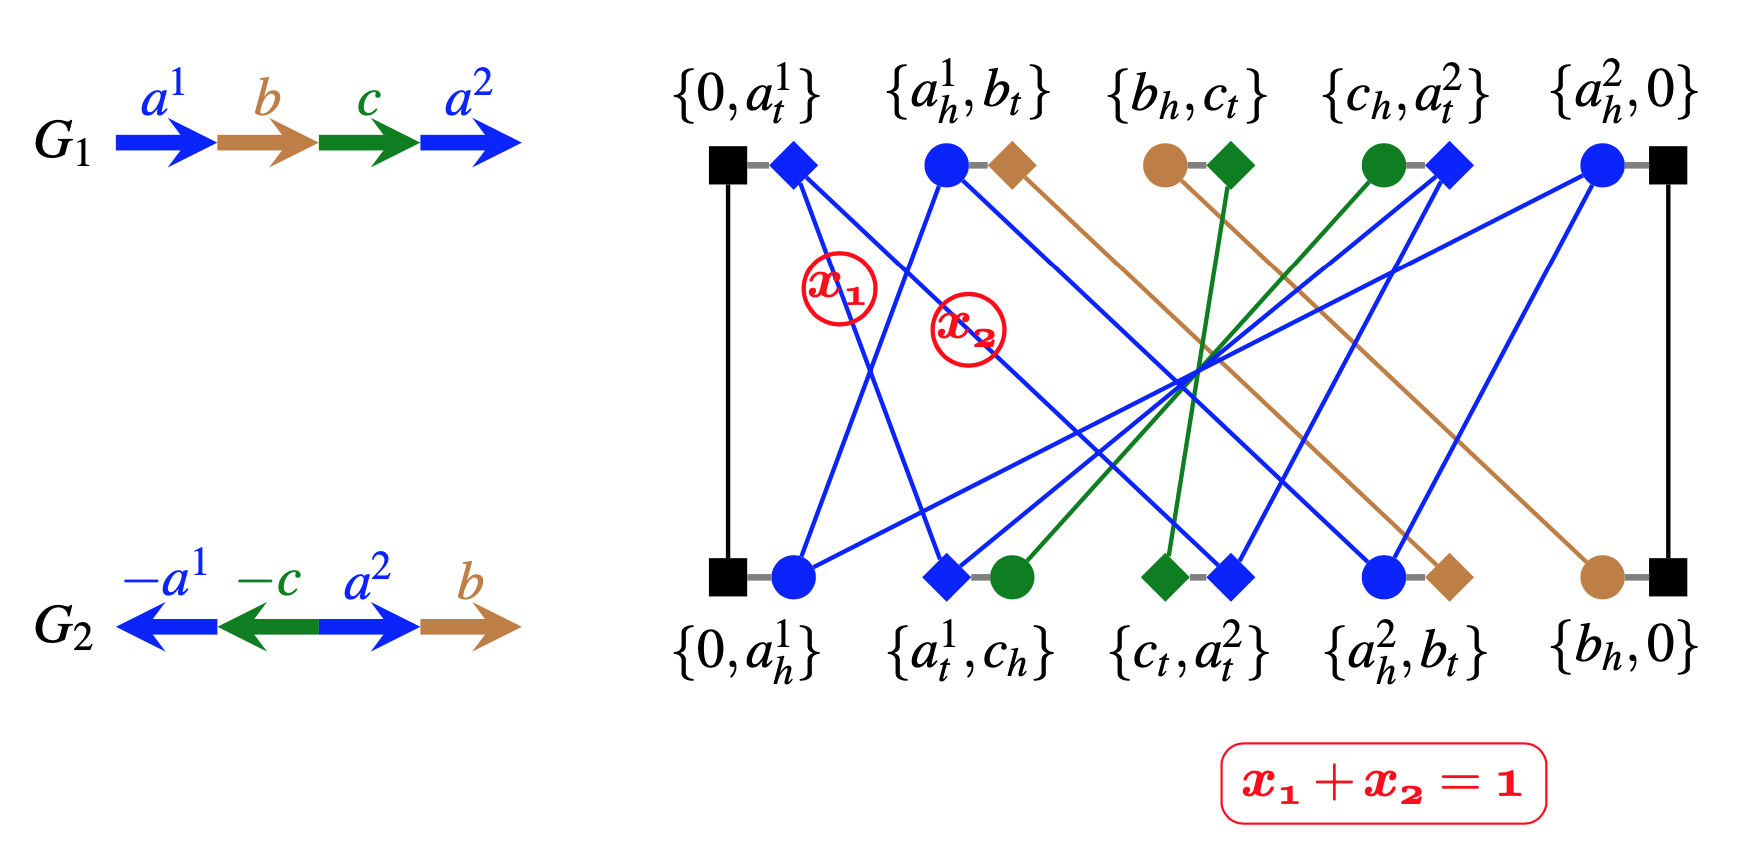
\includegraphics[width=0.7\textwidth]{L8-DCJ7.png}
	\end{center}

	\begin{itemize}
	\item<1-> Variables: $x_e\in\{0,1\}$, indicating choosing $e$ or not
	\vspace{0.1cm}
	\item<1-> Constraints: ensure a one-to-one correspondence
	\end{itemize}
}

\frame
{
	\frametitle{ILP Formulation}

	\begin{center}
		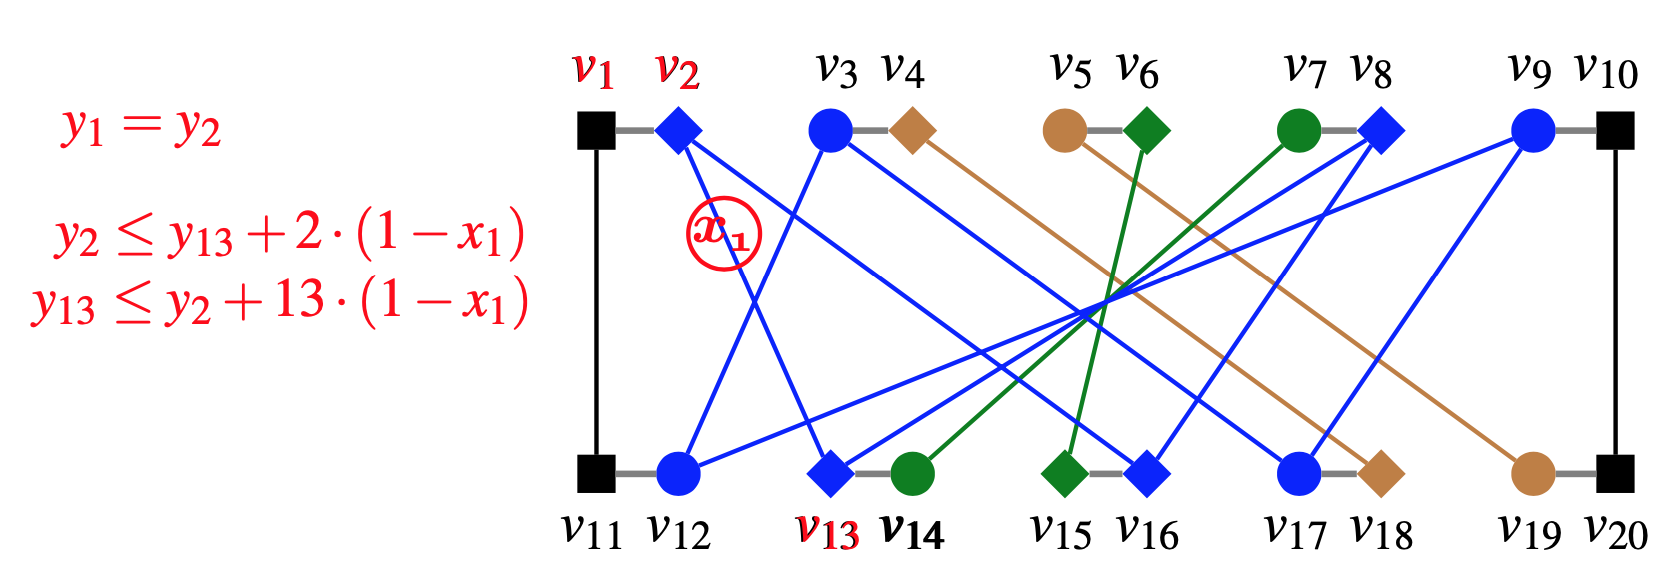
\includegraphics[width=0.7\textwidth]{L8-DCJ8.png}
	\end{center}

	\begin{itemize}
	\item Variables: $y_i \in [1, \mathbold{\textcolor{red}i}]$, representing the label of $v_i$
	\item Constraints: 
		\begin{itemize}
			\item Two vertices inside one adjacency always have the same label.
			\item Vertices connected by chosen edges have the same label.
		\end{itemize}
		
		\item $\rightarrow$ For any feasible solution, all vertices in the same cycle (induced by the solution) must have the same label.
		\item $\rightarrow$ At most one vertex in each cycle can reach the upper bound.
	\end{itemize}
}

\frame
{
	\frametitle{ILP Formulation}
	\vspace{-0.2cm}
	\begin{itemize}
	\item<1-> Variables: $z_i \in \{0,1\}$, indicating whether $y_i = i$
	\vspace{0.3cm}
	\item<1-> Constraints: ensure that $z_i = 1$ only if $y_i = i$
		$$i\cdot z_i \le y_i,\quad 1 \le i \le |V|$$
	\item<1-> Objective: maximize the number of cycles
		$$\max \sum_{1\le i \le |V|} z_i$$
	\vspace{0.3cm}
	\item<1-> $O(|E|)$ variables and $O(|E|)$ constraints
	\end{itemize}
}


\frame{
\begin{block}{}
 A brief history of linear programming
 \end{block}
}



\frame{
\frametitle{Concept, algorithms and analysis}

\begin{itemize}
 \item In 1939, L. Kantorovich proposed the concept of linear programming (called {\it extremal problem}) as mathematical formulation of practical problems in planned economy.  He also proposed the {\it resolving multiplier} approach. 
 \item In 1941, Hitchcock proposed the {\sc assignment} problem.
 \item In 1949, G. B. Dantzig advanced this concept and proposed the {\it simplex} algorithm. 
 \item In 1971, Klee and Minty gave a counter-example to show that simplex is not a polynomial-time algorithm.
 \item In 1975, L. V. Kantorovich, Nobel prize, application of linear programming in resource distribution;
 \item In 1979, L. G. Khanchian proposed a polynomial-time ellipsoid method;
 \item In 1984, N. Karmarkar proposed another polynomial-time interior-point method;
 \item In 2001, D. Spielman and S. Teng proposed smoothed complexity to prove the efficiency of simplex algorithm.
\end{itemize}
}

\frame{
	\frametitle{L. Kantorovich} 

\begin{figure}
 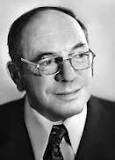
\includegraphics[width=1.2in] {Kantorovich.jpeg}
\caption{Leonid Kantorovich}
\end{figure}

L. Kantorovich was known for his theory and development of techniques for the optimal allocation of resources. He is regarded as the founder of linear programming. He was the winner of the Stalin Prize in 1949 and the Nobel Memorial Prize in Economics in 1975.
} 

\frame{
\frametitle{George B. Dantzig proposed LP model in 1947 }

\begin{figure}
 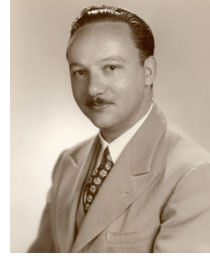
\includegraphics[width=1.2in] {Dantzig.jpg}
\end{figure}

\begin{itemize}
\begin{footnotesize}
 \item In 1946, as mathematical adviser to the U.S. Air Force Comptroller, he was challenged by his Pentagon colleagues to see what he could do to mechanize the planning process, "to more rapidly compute a time-staged deployment, training and logistical supply program."
\item In those pre-electronic computer days, mechanization meant using analog devices or punched-card machines. "Program" was a military term referring not to the instruction used by a computer to solve problems (called "codes"), but rather to plans or proposed schedules for training, logistical supply, or deployment of combat units.
\end{footnotesize}
\end{itemize}

}


\frame[allowframebreaks]{
\frametitle{LP is in $P$}

\begin{figure}
 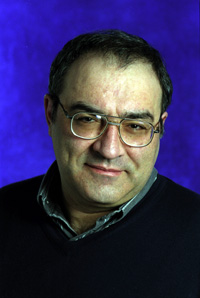
\includegraphics[width=1.5in] {L8-Khachiyan.jpg}
\caption{Leonid G. Khanchian}
\end{figure}

\begin{figure}
 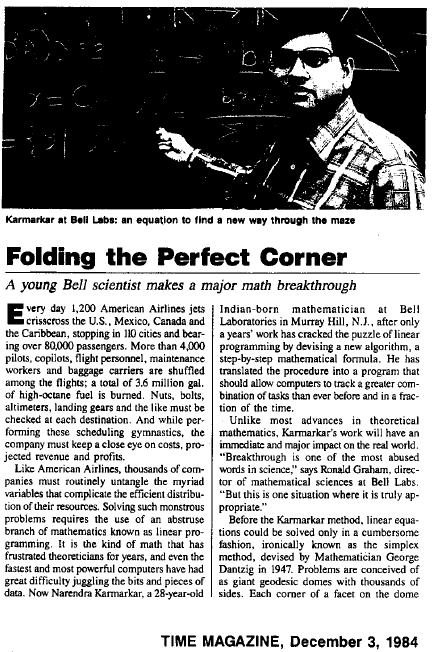
\includegraphics[width=3in] {L8-Karmarkar.png}
 \caption{N. Karmarkar}
\end{figure}
} 

\frame{
\frametitle{NLP, Convex Programming, LP, Network flow, and ILP.}
\begin{figure}
 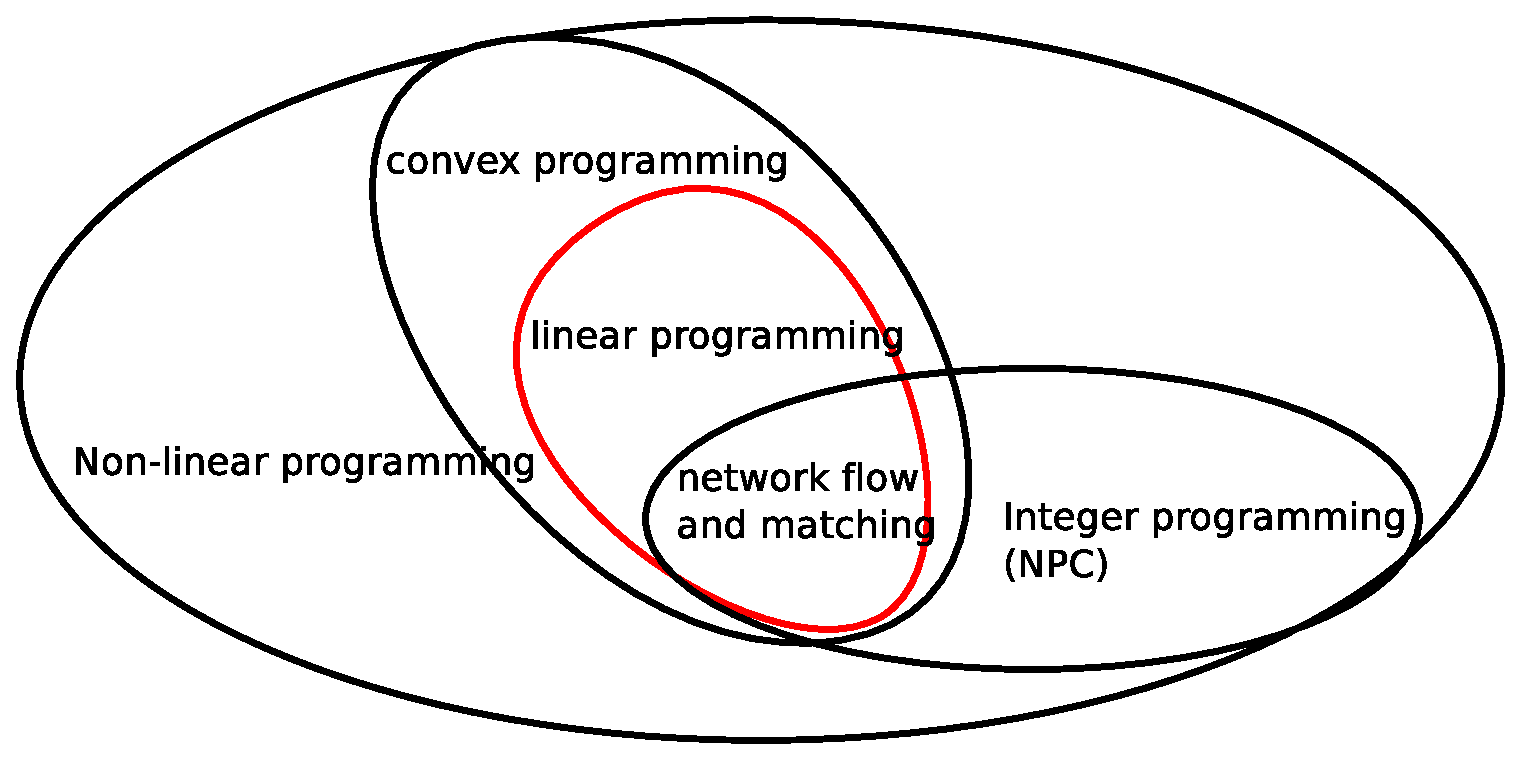
\includegraphics[width=3.5in] {L8-NLPLP.eps}
\end{figure}
Notes:
\begin{enumerate}
 \item In convex programming, local optimum is also global optimum.
 \item {\sc Network Flow} and {\sc Matching} are special ILP problems: the special problem structure determines that an LP model can automatically generate integral solutions.
\end{enumerate}
}


\frame{
\frametitle{GLPK: an efficient LP solver }
\begin{itemize}
 \item
The GLPK (GNU Linear Programming Kit, http://www.gnu.org/software/glpk/) package is intended for solving large-scale linear programming (LP), mixed integer programming (MIP), and other related problems. It is a set of routines written in ANSI C and organized in the form of a callable library.
\item
GLPK supports the GNU MathProg modeling language, which is a subset of the AMPL language.
\item
The GLPK package includes the following main components:
\begin{enumerate}
\item     primal and dual simplex methods
    \item  primal-dual interior-point method
    \item  branch-and-cut method
    \item  translator for GNU MathProg
    \item  application program interface (API)
\item      stand-alone LP/MIP solver
\end{enumerate}
\end{itemize}
(See extra slides)
}

\frame{
\frametitle{Gurobi: Outstanding solver}

\begin{itemize}
\item 
The Gurobi Optimizer (http://gurobi.com) is a state-of-the-art solver for mathematical programming. It includes the following solvers: linear programming solver (LP solver), quadratic programming solver (QP solver), quadratically constrained programming solver (QCP solver), mixed-integer linear programming solver (MILP solver), mixed-integer quadratic programming solver (MIQP solver), and mixed-integer quadratically constrained programming solver (MIQCP solver)
\item The solvers in the Gurobi Optimizer were designed from the ground up to exploit modern architectures and multi-core processors, using the most advanced implementations of the latest algorithms.
\end{itemize}
}




\frame{
\begin{block}{}
Various linear program forms: general form, standard form, and slack form.
\end{block}
}

\frame{
\frametitle{Form 1. General form of linear programming }
\begin{itemize}
\item 
General form: mixture of linear inequalities and equalities
\[
\begin{array}{rrrrrrrrrrrrl}\nonumber
 \min & c_1x_1    &+&  c_2x_2   &+&  ...&+& c_nx_n    &      &     & \\
 s.t. & a_{i1}x_1 &+& a_{i2}x_2 &+& ... &+& a_{in}x_n & \geq & b_i & i \in M\\
      %&           & &           & & ... & &           &        &          &\\
      & a_{j1}x_1 &+& a_{j2}x_2 &+& ... &+& a_{jn}x_n &  =   & b_j & j \in \overline{M} \\
      &           & &           & &     & &       x_i & \geq & 0   & i \in N 
 %     &           & &           & &     & &       x_j &\leq\geq & 0 & j \in \overline{N} \\
     \end{array} \nonumber
\]
\end{itemize}
}

\frame{
\frametitle{Form 2: Standard form of linear programming }
\begin{itemize}
 \item
Standard form: linear inequalities;
\[
\begin{array}{rrrrrrrrrrrrl}
 \min & c_1x_1    &+&  c_2x_2   &+&  ...&+& c_nx_n    &      &    & \\
 s.t. & a_{11}x_1 &+& a_{12}x_2 &+& ... &+& a_{1n}x_n & \textcolor{red}{\leq} & b_1 &  \\
      & a_{21}x_1 &+& a_{22}x_2 &+& ... &+& a_{2n}x_n & \textcolor{red}{\leq} & b_2 &  \\
      &   ...    & &   ...   & & ... & & ... &      &     &  \\
      & a_{m1}x_1 &+& a_{m2}x_2 &+& ... &+& a_{mn}x_n & \textcolor{red}{\leq} & b_m &  \\
      &           & &           & &     & &       x_i & \geq & 0   & \text{for } \forall i
     \end{array} \nonumber
\]
\item
Standard form in matrix language:
\[
\begin{array}{rrrrrrrrrrrrl}
 \min & \mathnormal{c^Tx} &  &  \\
 s.t. & \mathnormal{Ax } & \leq & b \\
      & \mathnormal{x} & \geq & 0 \\
\end{array} \nonumber
\]
\item Here we assume the matrix $\mathnormal{A}$ has a full row rank. Otherwise a preprocessing step can be executed to guarantee this. 
\end{itemize}
}

\frame{
\frametitle{Standard form   }

\begin{itemize}
	\item 
	Standard form in matrix language:
\[
\begin{array}{rrrrrrrrrrrrl}
 \min & \mathnormal{c^Tx} &&    \\
 s.t. & \mathnormal{Ax} & \leq & b \\
      & \mathnormal{x} & \geq & 0 \\
\end{array} \nonumber
\]

\item Here 
$\mathnormal{c} = \left(
	   \begin{array}{c}
		 c_1 \\
	  	        c_2\\
	                                \vdots \\
	                         c_n 
	      \end{array}
	      \right) $, 
	$\mathnormal{x} = \left(
	   \begin{array}{c}
		 x_1 \\
	  	        x_2\\
	                                \vdots \\
	                         x_n 
	      \end{array}
	      \right) $, \\
			      $\mathnormal{A}=\left( 
	\begin{array}{cccc}
	a_{11} & a_{12} & \cdots & a_{1n} \\
	a_{21} & a_{22} & \cdots & a_{2n} \\
	\vdots & \vdots & \ddots & \vdots \\ 
	a_{m1} & a_{m2} & \cdots & a_{mn} 
	\end{array}
	\right)$,
	$\mathnormal{b} = \left(
	   \begin{array}{c}
		 b_1 \\
	  	        b_2\\
	                                \vdots \\
	                         b_m 
	      \end{array}
	      \right) $.
 	      
	                             
\end{itemize}

} 

\frame{
\frametitle{Transformation from general form to standard form}
\begin{itemize}
\item  Transformations:
\begin{enumerate}
\item \textcolor{red}{\bf Variables:}  a free variable $\Rightarrow$  two non-negativeive variables; \\
$x_i$ may or may not be positive  $\Rightarrow$  replacing $x_i$ with $x_i' - x_i''$ \\
     and adding constraints: $x_i' \geq 0 ; x_i'' \geq 0$
\ \\
\ \\
 \item \textcolor{red}{\bf Constraints:}  an equality $\Rightarrow$ two inequalities; \\
 $a_{j1}x_1 + a_{j2}x_2 + ... + a_{jn}x_n  \textcolor{red}{=}  b_j \Rightarrow $\\
$a_{j1}x_1 + a_{j2}x_2 + ... + a_{jn}x_n  \textcolor{red}{\geq} b_j $\\
$a_{j1}x_1 + a_{j2}x_2 + ... + a_{jn}x_n  \textcolor{red}{\leq} b_j $
\end{enumerate}
\end{itemize}
}


\frame{
\frametitle{Form 3: Slack form of linear programming }

\begin{itemize}
\item
Slack form: linear equality;
\[
\begin{array}{rrrrrrrrrrrrl}
 \min & c_1x_1    &+&  c_2x_2   &+&  ...&+& c_nx_n    &      &    & \\
 s.t. & a_{11}x_1 &+& a_{12}x_2 &+& ... &+& a_{1n}x_n & \textcolor{red}{=} & b_1 &  \\
      & a_{21}x_1 &+& a_{22}x_2 &+& ... &+& a_{2n}x_n & \textcolor{red}{=} & b_2 &  \\
      &  ... & &   ... & & ... & &  ...  &      &     &  \\
      & a_{m1}x_1 &+& a_{m2}x_2 &+& ... &+& a_{mn}x_n & \textcolor{red}{=} & b_m &  \\
      &           & &           & &     & &       x_i & \geq & 0   & \text{for } \forall i 
     \end{array} \nonumber
\]
\item
Slack form in matrix language:
\[
\begin{array}{rrrrrrrrrrrrl}
 \min & \mathnormal{c^Tx}   \\
 s.t. & \mathnormal{Ax = b} \\
      & \mathnormal{x \geq} 0 \\
\end{array} \nonumber
\]
\end{itemize}
}

\frame{
\frametitle{Transformation from standard form to slack form }
\begin{itemize}
\item 
Transformations: 
\begin{enumerate}
 \item
\textcolor{red}{\bf Variables:} changing ``inequality on partial solution $(x_1,...,x_n)$'' to ``equality on full solution $(\textcolor{red}{s}, x_1, ..., x_n)$'' by introducing a slack variable $s$. \\
$a_{j1}x_1 + a_{j2}x_2 + ... + a_{jn}x_n  \textcolor{red}{  \leq } b_j \Rightarrow $\\
$a_{j1}x_1 + a_{j2}x_2 + ... + a_{jn}x_n  \textcolor{red}{ + s = } b_j $\\
\ \\
\ \\
\item
\textcolor{red}{\bf Constraint:}  $s \geq 0 $.  ($s$ is called a slack variable)
\end{enumerate}
\end{itemize}
}

\frame{
\frametitle{Example:  standard form vs. slack form  }
\begin{itemize}
\item 
Standard form:
\[
\begin{array}{rrrrrrrrrrrrl}
            & &             &-&x_3     &+&2x_4  & \textcolor{red}{\leq} & 2 &  \\
             & &           & & 3x_3  &-&2x_4  &  \textcolor{red}{\leq} & 6 &  \\
        & &  & & x_{3}&,&x_{4} &  \geq  & 0 & \\
     \end{array} \nonumber
\]

\item 
Slack form:
\[
\begin{array}{rrrrrrrrrrrrl}
     \textcolor{red}{  x_1 }& &             &-& x_3     &+&2x_4  & \textcolor{red}{=} & 2 &  \\
             & & \textcolor{red}{  x_{2} }   &+& 3x_3  &-&2x_4  &\textcolor{red}{=}& 6 &  \\
      \textcolor{red}{ x_1} &,& \textcolor{red}{ x_2} &,& x_{3}&,&x_{4} &  \geq  & 0 & \\
     \end{array} \nonumber
\]

\end{itemize}

}


%\frame{
%	\frametitle{Solving strategy I}
%
%\[
%\begin{array}{rrrrl}
% \max & c_1 +&  c_2 +& c_3 & \\
% s.t. & x_1 +& (1-x_2) +& x_3 & \geq c_1 \\
%      & (1-x_1) +&  x_2 +& (1-x_3) & \geq c_2 \\
%      & x_1 +&  x_2 +& (1-x_3) & \geq c_3 \\
%      & x_1 ,& x_2 ,& x_3 & = 0/1 \\
%      & c_1 ,& c_2 ,& c_3 & = 0/1
%\end{array} \nonumber
%\]
%	\begin{itemize}
%		\item Solution: $X=[x_1, x_2, ..., x_n]$, $x_i = 0/1$ 
%		\item Partial solution enumeration tree: 
%	\begin{center}
%		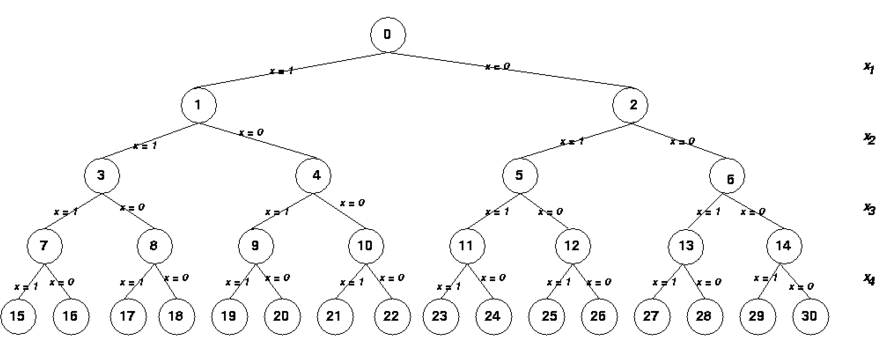
\includegraphics[width=0.6\textwidth]{Branch-and-bound1.png}
%	\end{center}			
%		\item We will talk about ``intelligent enumeration", say branch-and-bound, and backtracking, later. 
%	\end{itemize}
%	
%} 
%
%\frame{
%	\frametitle{Solving strategy II}
%
%	\begin{itemize}
%		\item Solution: $x=(x_1, x_2, ..., x_n)$ 
%		\item Complete solution landscape 
%	\begin{center}
%		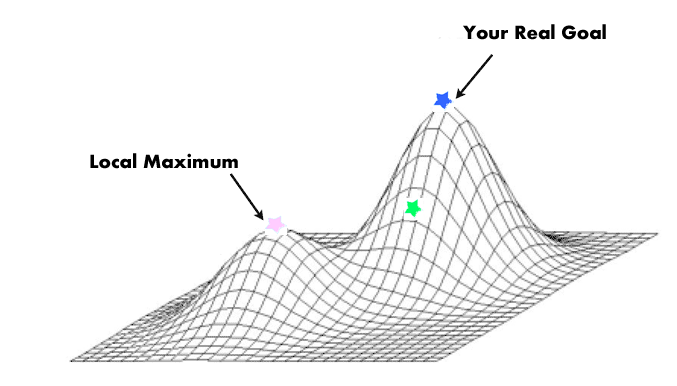
\includegraphics[width=0.6\textwidth]{ImprovementStrategy.png}
%	\end{center}
%						
%		\item Each node represents a complete solution, and two solutions are called 
%		neighbours if one solution can be obtained 
%		from another with a small change. 
%	\end{itemize}
%	
%} 
%

\frame{
\begin{block}{}
Intuition of linear programming\\
\end{block}

}

\frame{
\frametitle{Two differences from linear equation formula }
\begin{itemize} 
\item 
Consider a LP (in slack form): 
\[
\begin{array}{rrrrrrrrrrrrl}
 \min & \mathnormal{c^Tx}  & &  \\
 s.t. & \mathnormal{Ax } &=& b \\
      & \mathnormal{x} &  \geq & 0 \\
\end{array} \nonumber
\]
\item 
We have already known how to solve $\mathnormal{Ax=b}$. 
\item 
What is the difference between LP and linear equation formula?
\begin{enumerate}
 \item Constraints: $\mathnormal{x} \geq 0$;
 
 \item Objective function: $\min$ $\mathnormal{c^Tx}$;

\end{enumerate}
\end{itemize} 
}

\frame{
	\begin{block}{}
	The effect of constraints  $\mathnormal{x} \geq 0$
	\end{block}
}

\frame{
\frametitle{Revisiting $\mathnormal{Ax=b}$ }
\begin{itemize} 
\item An example of $\mathnormal{Ax=b}$ 
\[
\begin{array}{rrrrrrrrrrrrl}
      x_1 & &             &-& x_3     &+&2x_4  & \textcolor{red}{=} & 2 &  \\
             & & x_{2}    &+& 3x_3  &-&2x_4  &\textcolor{red}{=}& 6 &  \\
       2x_1     &+ & x_{2}    &+& x_3  &+&2x_4  &\textcolor{red}{=}& 10 &  
     \end{array} \nonumber
\]
\item By applying Gaussian elimination, we have: 
\[
\begin{array}{rrrrrrrrrrrrl}
      x_1 & &             &-& x_3     &+&2x_4  & \textcolor{red}{=} & 2 &  \\
             & & x_{2}    &+& 3x_3  &-&2x_4  &\textcolor{red}{=}& 6 &  \\
     \end{array} \nonumber
\]
\item  Intuitively, \textcolor{red}{\bf any point} in the $(x_3, x_4)$ plane corresponds to a full solution $(x_1, x_2, x_3, x_4)$. 
\begin{figure}%
      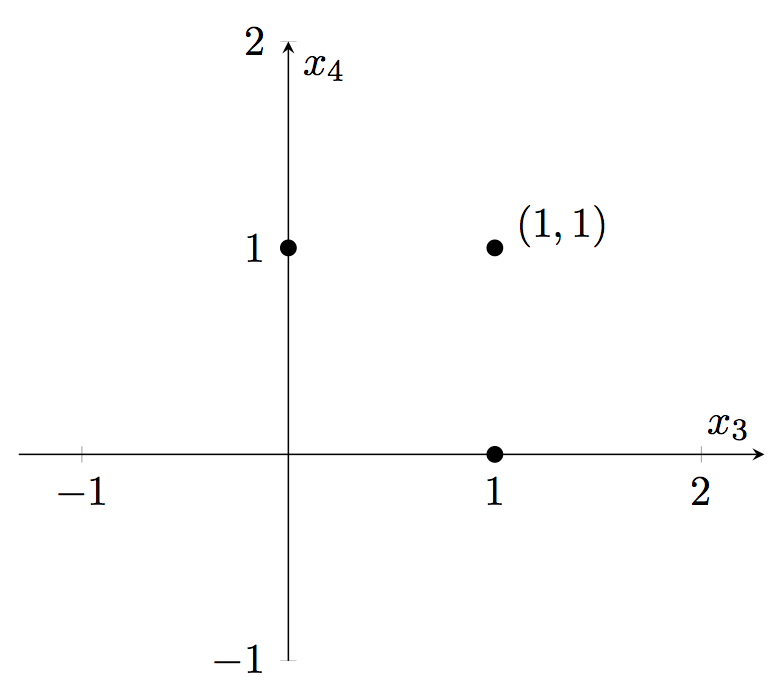
\includegraphics[width=1.5in]{L8-LEexample.png}%
 \end{figure}
\end{itemize} 

} 

\frame{
\frametitle{The effect of $\mathnormal{x} \geq 0$  }

\begin{itemize} 
\item An example of $\mathnormal{Ax=b, x} \geq 0$ 
\[
\begin{array}{rrrrrrrrrrrrl}
      x_1 & &             &-& x_3     &+&2x_4  & \textcolor{black}{=} & 2 &  \\
             & & x_{2}    &+& 3x_3  &-&2x_4  &\textcolor{black}{=}& 6 &  \\
       2x_1     &+ & x_{2}    &+& x_3  &+&2x_4  &\textcolor{black}{=}& 10 &  \\
              \textcolor{red}{x_1} &\textcolor{red}{,}& \textcolor{red}{x_2}&\textcolor{red}{,}& \textcolor{red}{x_{3}}&\textcolor{red}{,}&\textcolor{red}{x_{4}} &  \geq  & \textcolor{red}{0} & \\
     \end{array} \nonumber
\]
\item By applying Gaussian elimination, we have: 
\[
\begin{array}{rrrrrrrrrrrrl}
      x_1 & &             &-& x_3     &+&2x_4  & \textcolor{black}{=} & 2 &  \\
             & & x_{2}    &+& 3x_3  &-&2x_4  &\textcolor{black}{=}& 6 &  \\
              \textcolor{red}{x_1} &\textcolor{red}{,}& \textcolor{red}{x_2}&\textcolor{red}{,}& \textcolor{red}{x_{3}}&\textcolor{red}{,}&\textcolor{red}{x_{4}} &  \textcolor{red}{\geq}  & \textcolor{red}{0} & \\
     \end{array} \nonumber
\]
\item This is essentially a \textcolor{red}{\bf linear inequality formula}: 
\[
\begin{array}{rrrrrrrrrrrrl}
            & &             &-& x_3     &+&2x_4  & \textcolor{blue}{\bf \leq} & 2 &  \\
             & &           & & 3x_3  &-&2x_4  &  \textcolor{blue}{\bf \leq} & 6 &  \\
             & & & & \textcolor{red}{x_{3}}&\textcolor{red}{,}&\textcolor{red}{x_{4}} &  \textcolor{red}{\geq}  & \textcolor{red}{0} & \\
     \end{array} \nonumber
\]
\end{itemize} 

}


\frame{
\frametitle{The effect of $\mathnormal{x \geq} 0$ cont'd }

\begin{itemize} 
\item Linear inequality formua: 
\[
\begin{array}{rrrrrrrrrrrrl}
            & &             &-& x_3     &+&2x_4  & \textcolor{blue}{\bf \leq} & 2 &  \\
             & &           & & 3x_3  &-&2x_4  &  \textcolor{blue}{\bf \leq} & 6 &  \\
             & & & & \textcolor{red}{x_{3}}&\textcolor{red}{,}&\textcolor{red}{x_{4}} &  \textcolor{red}{\geq}  & \textcolor{red}{0} & \\
     \end{array} \nonumber
\]
\item  Any point in \textcolor{red}{\bf  the polytope} rather than \textcolor{red}{\bf the whole plane}   corresponds to a feasible solution, e.g.  $(x_{3}, x_{4})=(1,1)$ corresponds to $(x_{1}, x_{2}, x_{3}, x_{4}) = (1, 5, 1, 1)$.
\end{itemize} 

\begin{figure}%
      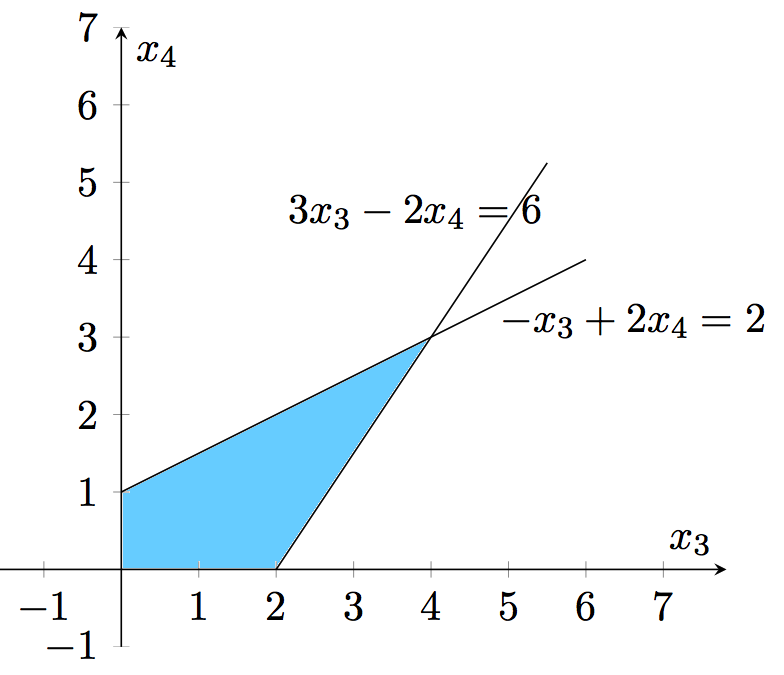
\includegraphics[width=2in]{L8-LP-GE.png}%
 \end{figure}

}



\frame{
\frametitle{Polytope $\Leftrightarrow$ feasible region}
\begin{Theorem}
\textcolor{red}{\bf Any polytope} $\mathnormal{P} \subset \mathbb{R}^{n-m}$ corresponds to the feasible region of a linear program $\mathnormal{Ax=b, x}\geq 0$ (denoted as $F=\{\mathnormal{x \ | \  Ax=b, x}\geq 0 \}$), and vice versa.
\end{Theorem}
\begin{itemize}
\item 
Basic idea: What is the effect of constraint $\mathnormal{ x\geq 0}$? It implies the interchangeability between \textcolor{red}{\bf equalities on all variables} ( e.g. $x_2 + 3x_3  - 2x_4  \textcolor{blue}{=}  6$)  and \textcolor{red}{\bf inequalities on partial variables} (e.g. $ 3x_3  - 2x_4  \textcolor{blue}{\leq}  6$).
\end{itemize}


}

\frame{
\frametitle{Proof: feasible region $\Rightarrow$ polytope}
\begin{itemize}
\item 
Basic idea: changing \textcolor{red}{\bf equality} to \textcolor{red}{\bf  inequality} through Gaussian row operations followed by removing some variables.\\

 \item
Consider a \textcolor{red}{\bf feasible full solution  $\mathnormal{x}$ } of the following LP:
\begin{small}
\[
\begin{array}{rrrrrrrrrrrrl}
   & a_{11}x_1 &+& a_{12}x_2 &+& ... &+& a_{1n}x_n & = & b_1 &  \\
   & a_{21}x_1 &+& a_{22}x_2 &+& ... &+& a_{2n}x_n & = & b_2 &  \\
   &           & &           & & ... & &           &      &     &  \\
   & a_{m1}x_1 &+& a_{m2}x_2 &+& ... &+& a_{mn}x_n & = & b_m &  \\
   & x_1 &,& x_2 &,& ... &,& x_n & \geq & 0 &  \\
\end{array} \nonumber
\]
\end{small}
\item
Applying Gaussian row operations, we have:
\begin{small}
\[
\begin{array}{rrrrrrrrrrrrrrrrrl}
   & x_1 & &     & &     &+& a_{1,m+1}'x_{m+1} &+& ... &+& a_{1n}'x_n & = & b_1' &  \\
   &     & & x_2 & &     &+& a_{2,m+1}'x_{m+1} &+&... &+& a_{2n}'x_n & = & b_2' &  \\
   &     & &  ...& &     & & ... & &           &      &     &  \\
   &     & &     & & x_m &+& a_{m,m+1}'x_{m+1}&+&... &+& a_{mn}'x_n & = & b_m' &  \\
   & x_1 &,& x_2 &,& x_m &,& x_{m+1}&,&... &,& x_n & \geq & 0 &  \\
\end{array} \nonumber
\]
\end{small}
\end{itemize}
}

\frame{
\frametitle{Proof: feasible region $\Rightarrow$ polytope cont'd}
\begin{itemize}

\item
By \textcolor{red}{\bf removing  positive variables $x_1, x_2,..., x_m$}, we have the following \textcolor{red}{\bf linear inequalities}: 
\[
\begin{array}{rrrrrrrrrrrrrrrrrl}
    a_{1,m+1}'x_{m+1} &+& ... &+& a_{1n}'x_n & \textcolor{blue}{\bf \leq} & b_1' &  \\
   a_{2,m+1}'x_{m+1} &+&... &+& a_{2n}'x_n & \textcolor{blue}{\bf \leq} & b_2' &  \\
    & &   ...        &      &     &  \\
    a_{m,m+1}'x_{m+1}&+&... &+& a_{mn}'x_n & \textcolor{blue}{\bf \leq} & b_m' &  \\
    x_{m+1}&,&... &,& x_n & \geq & 0 &  \\
\end{array} \nonumber
\]
\item Define  a polytope $\mathnormal{P} \subset \mathbb{R}^{n-m}$  as the intersection of $m$ half-spaces:

$HS_j: a_{j,m+1}'x_{m+1} + ... + a_{jn}'x_n \textcolor{blue}{\bf \leq } b_j' $ , $1\leq j \leq m$. (by $x_j \geq 0$)

\item
Thus,  \textcolor{red}{\bf any feasible full solution }  $\mathnormal{x} = (x_1, x_2, ..., x_n)$   $\Rightarrow$ \textcolor{red}{\bf partial  solution  } $ \mathnormal{{x}_{N}}=(x_{m+1}, ..., x_n)\in \mathnormal{P}$.
\end{itemize}
}

\frame{
\frametitle{Proof:  polytope $\Rightarrow$  feasible region}
\begin{itemize}
\item 
Basic idea:  changing \textcolor{red}{\bf inequality} to \textcolor{red}{\bf equality} through introducing \textcolor{red}{\bf slack variables.}  \\

\begin{itemize}
 \item

Suppose $P$ is the intersection of $m$ half-spaces (inequalities), say:

$HS_j: a_{j1}x_1 + a_{j2}x_2 + ... + a_{jn}x_n \textcolor{blue}{ \leq } b_j $ ($1\leq j \leq m$)\\
\item Introducing a non-negative slack variable $s_j$ to each inequality, we have:\\
$\ \ \ \ \ \ a_{j1}x_1 + a_{j2}x_2 + ... + a_{jn}x_n +\textcolor{blue}{ s_j  = } b_j $ ($s_j \geq 0$)  \\

\end{itemize}
\end{itemize}
}

\frame{
\frametitle{Proof:  polytope $\Rightarrow$  feasible region    cont'd}
\begin{itemize}
\item Thus we change
\[
\begin{array}{rrrrrrrrrrrrl}
   & a_{11}x_1 &+& a_{12}x_2 &+& ... &+& a_{1n}x_n & \textcolor{blue}{\leq} & b_1 &  \\
   & a_{21}x_1 &+& a_{22}x_2 &+& ... &+& a_{2n}x_n & \textcolor{blue}{\leq} & b_2 &  \\
   &           & &           & & ... & &           &      &     &  \\
   & a_{m1}x_1 &+& a_{m2}x_2 &+& ... &+& a_{mn}x_n & \textcolor{blue}{\leq} & b_m &  \\
   & x_1 &,& x_2 &,& ... &,& x_n & \geq & 0 &  \\
\end{array} \nonumber
\]

into
\[
\begin{array}{rrrrrrrrrrrrrrrrrl}
   &\textcolor{blue}{s_1}  & &     & &     &+& a_{1,1}x_{1} &+& ... &+& a_{1n}x_n & \textcolor{blue}{=} & b_1 &  \\
   &     & & \textcolor{blue}{s_2}   & &     &+& a_{2,1}x_{1} &+&... &+& a_{2n}x_n & \textcolor{blue}{=}  & b_2 &  \\
   &     & &  ...& &     & & ... & &           &      &     &  \\
   &     & &     & & \textcolor{blue}{s_m}   &+& a_{m,1}x_{1}&+&... &+& a_{mn}x_n & \textcolor{blue}{=}  & b_m &  \\
   & \textcolor{blue}{s_1} &,& \textcolor{blue}{s_2} &,& \textcolor{blue}{s_m} &,& x_{1}&,&... &,& x_n & \geq & 0 &
\end{array} \nonumber
\]

\item  Thus, a \textcolor{red}{\bf partial  solution} $(x_1, x_2, ..., x_n) \in \mathnormal{P} \Rightarrow$ a \textcolor{red}{\bf feasible full solution} $(\textcolor{blue}{s_1,s_2,...,s_m}, x_1, x_2, ..., x_n) \geq 0$.
\end{itemize}
}



\frame{
\frametitle{Notations}

\begin{figure}
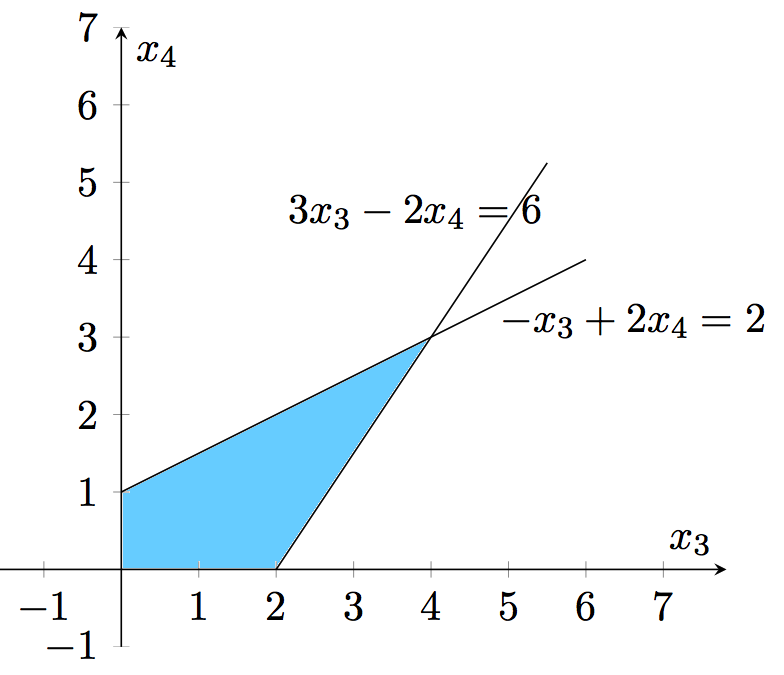
\includegraphics[width=2in] {L8-LP-GE.png}
\end{figure}
 
\begin{itemize}
 \item Hyper plane: $\{ \mathnormal{x} \ | \  a_1x_1 + a_2 x_2 + ... + a_n x_n = b \}$ (linear equality constraint)
 \item Half space: $\{ \mathnormal{x} \ | \  a_1x_1 + a_2 x_2 + ... + a_n x_n \leq {b} \}$ (linear inequality constraint)
 \item Polyhedron: the intersection of several half spaces;
 \item Polytope: a bounded, non-empty polyhedron;
\end{itemize}
% Suppose $P$ is a $d$-dimensional polytope, $HS$ is a half space determined by a hyper place $H$, if $f=P\cap HS \subset H$, $f$ is called
% \begin{itemize}
%  \item Plane: if $f$ has $d-1$ dimensions.
%  \item Edge: if $f$ has $1$ dimension.
%  \item Vertex: if $f$ has $0$ dimension.
% \end{itemize}
%
% \begin{figure}
% 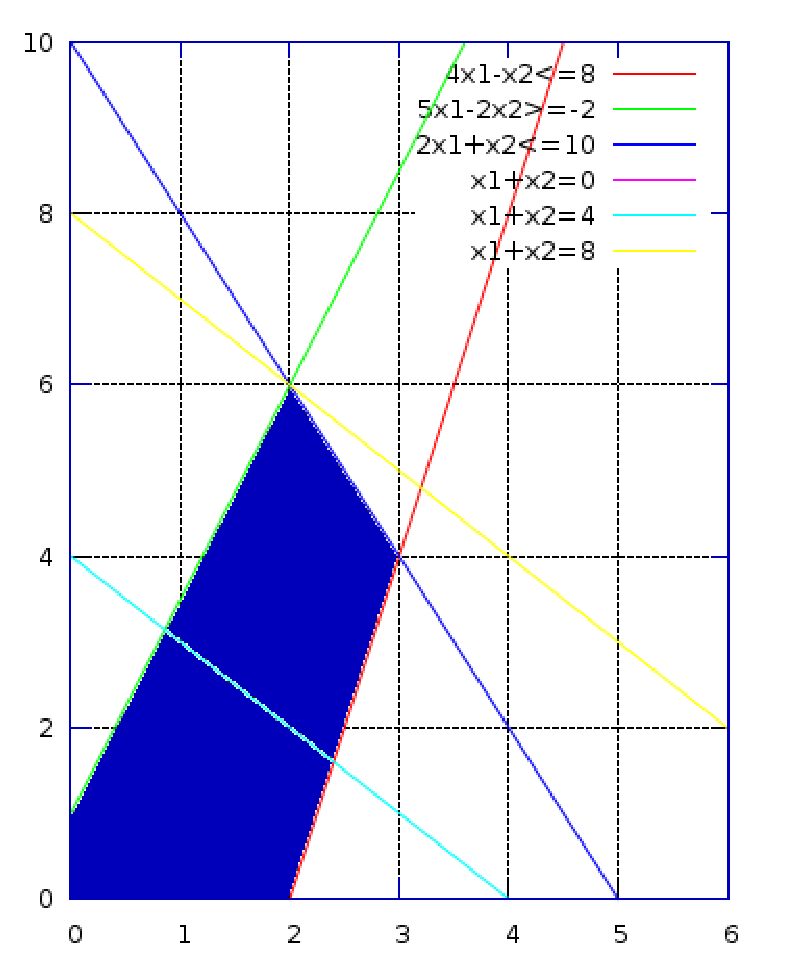
\includegraphics[width=1.3in] {L8-LPexample1.eps}
% \end{figure}
}


% \frame{
% \frametitle{feasible solution}
% \begin{itemize}
%  \item
% Suppose $rank(\mathnormal{A})=m$. Let us represent $\mathnormal{A}$ as $\mathnormal{A= [ B, N ] }$, where $\mathnormal{B=\{ \mathnormal{a}_1,  \mathnormal{a}_2, ...,  \mathnormal{a}_m } \}$ denotes a basis of $\mathnormal{A}$, and $\mathnormal{N}$ denotes the other columns in $\mathnormal{A}$.
% \item Gaussian elimination (essence:  multiplying by $\mathnormal{B^{-1} }$ on both sides ) changes
% \[
% \begin{array}{rrrrrrrrrrrrl}
%    & a_{11}x_1 &+& a_{12}x_2 &+& ... &+& a_{1n}x_n & = & b_1 &  \\
%    & a_{21}x_1 &+& a_{22}x_2 &+& ... &+& a_{2n}x_n & = & b_2 &  \\
%    &           & &           & & ... & &           &      &     &  \\
%    & a_{m1}x_1 &+& a_{m2}x_2 &+& ... &+& a_{mn}x_n & = & b_m &  \\
% \end{array} \nonumber
% \]
% to
% \[
% \begin{array}{rrrrrrrrrrrrrrrrrl}
%    & x_1 & &     & &     &+& a_{1,m+1}'x_{m+1} &+& ... &+& a_{1n}'x_n & =  b_1' &  \\
%    &     & & x_2 & &     &+& a_{2,m+1}'x_{m+1} &+&... &+& a_{2n}'x_n & =  b_2' &  \\
%    &     & &  ...& &     & & ... & &           &           &  \\
%    &     & &     & & x_m &+& a_{m,m+1}'x_{m+1}&+&... &+& a_{mn}'x_n & =  b_m' &  \\
% \end{array} \nonumber
% \]
% \item
% Setting non-basic variables  $\mathnormal{x_{N}= 0 }$, we can obtain $x_1=b_1', x_2=b_2',...,x_m=b_m'$, i.e.  $\mathnormal{x_B = B^{-1}b}$.
% \item  Thus the \textcolor{red}{full} solution is $\mathnormal{x= [x_B, x_{N}]=[B^{-1}b, 0]}$.
% \item If $\mathnormal{x_B = B^{-1}b \geq 0 }$, we call $\mathnormal{x}$  a {\bf basic feasible solution corresponding to $\mathnormal{B}$ } .
% \end{itemize}
% }



\frame{
	\begin{block}{}
	The effect of objective function   $\min \mathnormal{ c^T x}$
	\end{block}
}

\frame{
\frametitle{The effect of $\min \mathnormal{c^T x}$ }
\[
\begin{array}{rrrrrrrrrrrrl}
 \max & & &  & x_3    &+&  x_4   & &   & &      &      &     \\
   s.t.        & &             & &-x_3     &+&2x_4  & \textcolor{blue}{\leq} & 2 &  \\
             & &           & & 3x_3  &-&2x_4  &  \textcolor{blue}{\leq} & 6 &  \\
             & & & & \textcolor{red}{x_{3}}&\textcolor{red}{,}&\textcolor{red}{x_{4}} &  \textcolor{red}{\geq}  & \textcolor{red}{0} & \\
     \end{array} \nonumber
\]

\begin{figure}
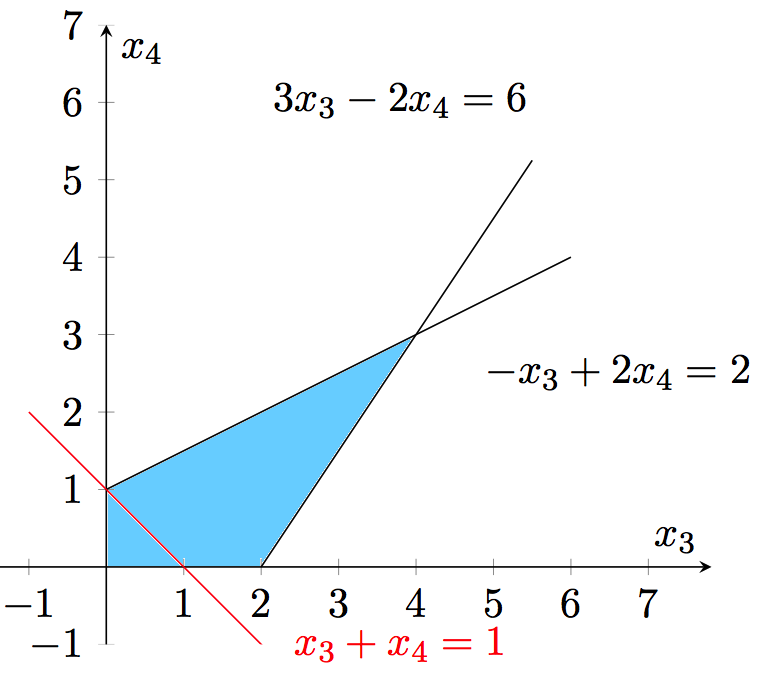
\includegraphics[width=2in] {L8-LP-GE1.png}
\end{figure}
 
}


\frame{
\frametitle{The effect of $\min \mathnormal{ c^T x}$  cont'd}
\[
\begin{array}{rrrrrrrrrrrrl}
 \max & & &  & x_3    &+&  x_4   & &   & &      &      &     \\
   s.t.        & &             & &-x_3     &+&2x_4  & \textcolor{blue}{\leq} & 2 &  \\
             & &           & & 3x_3  &-&2x_4  &  \textcolor{blue}{\leq} & 6 &  \\
             & & & & \textcolor{red}{x_{3}}&\textcolor{red}{,}&\textcolor{red}{x_{4}} &  \textcolor{red}{\geq}  & \textcolor{red}{0} & \\
     \end{array} \nonumber
\]

\begin{figure}
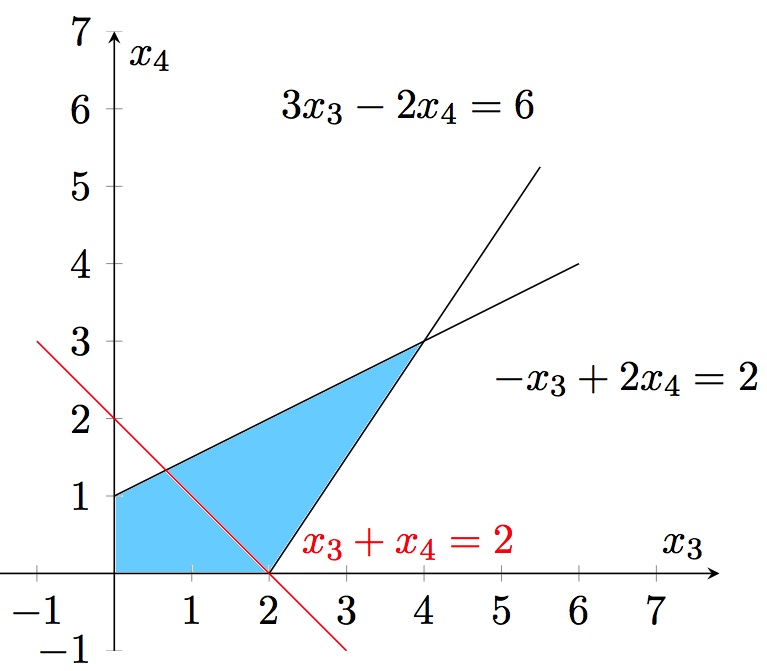
\includegraphics[width=2in] {L8-LP-GE2.png}
\end{figure}
 
}



\frame{
\frametitle{The effect of  $\min \mathnormal{ c^T x}$ cont'd }
\[
\begin{array}{rrrrrrrrrrrrl}
 \max & & &  & x_3    &+&  x_4   & &   & &      &      &     \\
   s.t.        & &             & &-x_3     &+&2x_4  & \textcolor{blue}{\leq} & 2 &  \\
             & &           & & 3x_3  &-&2x_4  &  \textcolor{blue}{\leq} & 6 &  \\
             & & & & \textcolor{red}{x_{3}}&\textcolor{red}{,}&\textcolor{red}{x_{4}} &  \textcolor{red}{\geq}  & \textcolor{red}{0} & \\
     \end{array} \nonumber
\]

\begin{figure}
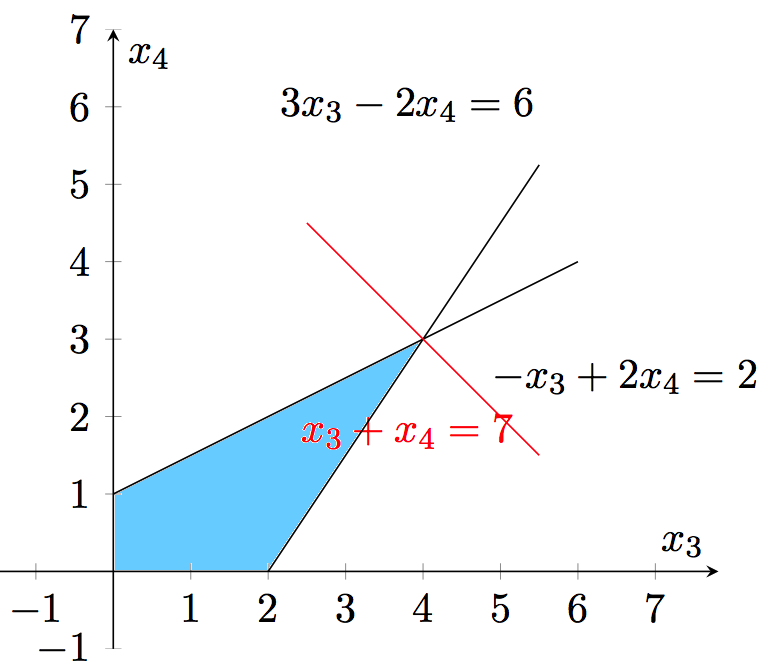
\includegraphics[width=2in] {L8-LP-GE3.png}
\end{figure}

\begin{itemize}
\item 
Observation: the optimal solution can be reached at a vertex of the polytope (if the optimal objective value is finite). 
 \end{itemize}
}


%
%\frame{
%\frametitle{Intuition of linear programming }
%\begin{enumerate}
%\item
%We have already known the Gaussian elimination technique to solve $\mathnormal{Ax=b}$. But now we have the constraints:  $\mathnormal{x}\geq 0$
%\item
%What is the effect of the constraint $\mathnormal{x}\geq 0$? The constraint implies the interchangeability between \textcolor{red}{\bf equalities on all variables} ( e.g. $x_2 + 3x_3  - 2x_4  \textcolor{blue}{=}  6$)  and \textcolor{red}{\bf inequalities on partial variables} (e.g. $ 3x_3  - 2x_4  \textcolor{blue}{\leq}  6$).
%\item
%Simplex algorithm can be treated as a \textcolor{red}{\bf Gaussian elimination on inequalities.}
%\end{enumerate}
%}
%

%
%
%\frame{
%\frametitle{Three issues in understanding linear programming }
%
% Three issues in understanding linear programming (by S. C. Fang and S. Puthenpura)
%\begin{enumerate}
% \item Geometric view: to get intuition;
% \item Algebra view: strict proof;
% \item Algorithm view: complexity.  \\
%\end{enumerate}
%}
%
%
%
%
%\frame{
%\begin{block}{}
%Linear programming properties: Geometric view
%\end{block}
%}
%
%
%\frame{
%\frametitle{An example and notations }
%
%\[
%\begin{array}{rrrrrrrrrrrrl}
% \min & -x_1    &-&  x_2   & &   & &      &      &    & \\
% s.t. & 4x_1 &-& x_2 & \leq & 8 &  \\
%      & 2x_1 &+& x_2 & \leq & 10 &  \\
%      & 5x_1 &-& 2x_2 & \geq & -2 &  \\
%      &  x_1 &,& x_2 & \geq  & 0 & \\
%     \end{array} \nonumber
%\]
%
%\begin{figure}
%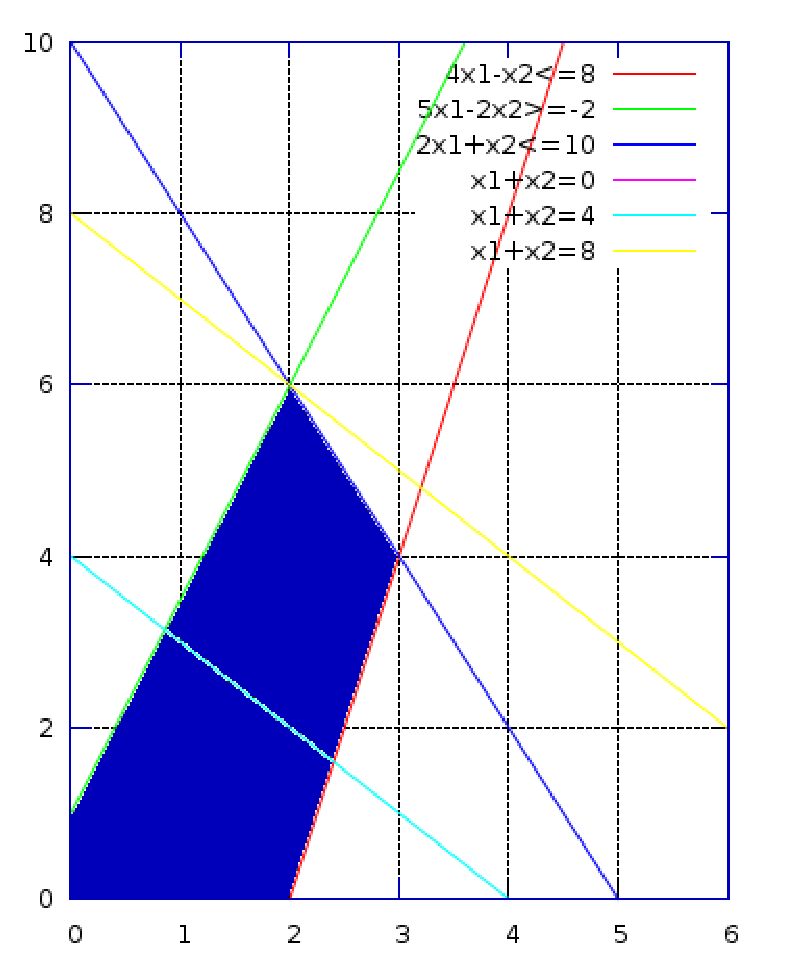
\includegraphics[width=1.5in] {L8-LPexample1.eps}
%\end{figure}
%}

\frame{
\frametitle{Key observations  of linear program}

\begin{figure}
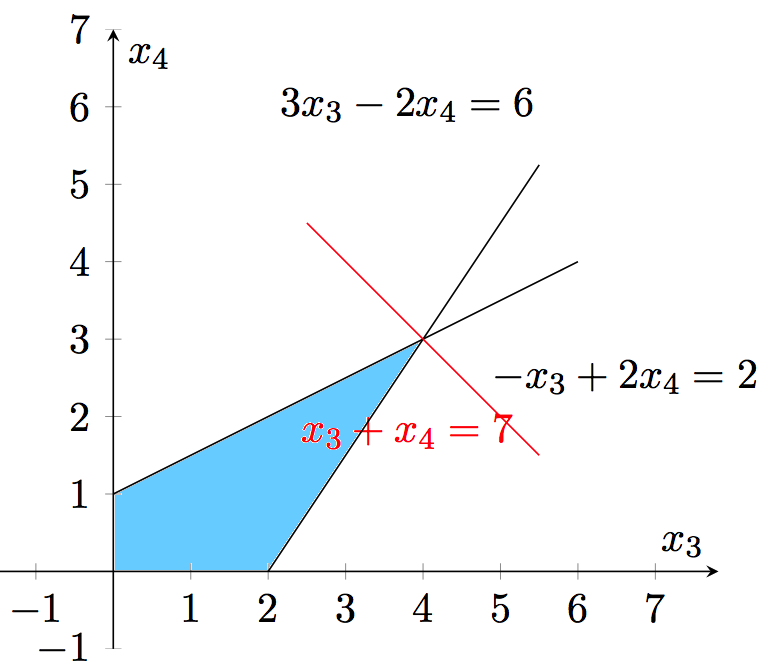
\includegraphics[width=2in] {L8-LP-GE3.png}
\end{figure}

\begin{enumerate}
 \item What is a feasible solution? Any point within the polytope. 
 \item Where is the optimal solution? A vertex of the polytope (if the optimal objective value is finite). Consequently, it is not necessary to 
 consider the inner points. In fact, the existence of a vertex solution makes the simplex algorithm distinctive from ellipsoid method and interior point method. 
 \end{enumerate}
}


\frame{
	\begin{block}{}
	{Applying the general {\sc Improvement} strategy to LP }
	\end{block}
}

\frame{
\frametitle{The general {\sc Improvement} strategy for optimization problems }
{\sc Improvement}$(f)$
\begin{algorithmic}[1]
\STATE $\mathnormal{x=x}_0$; //set initial solution;
\WHILE{  \texttt{TRUE} }
\STATE $\mathnormal{x}=${\sc Improve}$(\mathnormal{x}, f)$; //move towards optimum;  
\IF { {\sc stopping}$(\mathnormal{x}, f)$}  
\STATE break;
\ENDIF
\ENDWHILE
\RETURN $\mathnormal{x}$;
\end{algorithmic}

}


\frame{
\frametitle{Applying the general {\sc Improvement} strategy to LP }
\begin{tikzpicture}[x=0.7cm,y=0.7cm] 
%\pgfplotsset{my style/.append style={ axis x line=middle, axis y line=middle, axis equal }}

    \begin{axis}[anchor=origin,         xlabel=$x_3$,
        ylabel=$x_4$, 
        xtick={ 0,..., 5},
        ytick={ 0,..., 5}, 
        xmin=0,
        xmax=5,
        ymin=0,
        ymax=5, 
         x=0.7cm, y=0.7cm, 
        ];
              \addplot[domain=0:4.5]{0.5*x+1};
              \addplot[domain=2:5]{1.5*x-3};
%              \addplot[domain=-1:3,-,red]{-x+1};

		
      \end{axis};
                    \node at (6,3) {$-x_3+2x_4 = 2$};
              \node at (3,4) {$3x_3-2x_4 = 6$};
%              \node[red] at (4,0) {$x_3+x_4=1$};
	\draw[fill=green!20] (0, 0) -- ( 2, 0) -- (4,3) -- (0,1) -- (0,05);
	\node[circle, minimum size=3pt,inner sep=0pt, fill=red] at (0,0) {};
		\node[circle, minimum size=3pt,inner sep=0pt, fill=red] at (2,0) {};
			\node[circle, minimum size=3pt,inner sep=0pt, fill=red] at (4,3) {};
			\node[below, red, ultra thick] at (-0.2,-0.2) {start};
			\node[below, red, ultra thick] at (4.2,3) {end};	
			\draw[->, red, ultra thick] (0,0) -- (2,0); 
			\draw[->, red, ultra thick] (2,0) -- (4,3); 	
    \end{tikzpicture}
    
{\sc Improvement}()
\begin{algorithmic}[1]
\STATE $\mathnormal{x=x}_0$;  \textcolor{red}{//starting from a vertex;}
\WHILE{ \texttt{TRUE} }
\STATE $\mathnormal{x}=${\sc Improve}$(\mathnormal{x})$; \textcolor{red}{//move to another vertex via an edge;}
\IF { {\sc stopping}$(\mathnormal{x})$  }
\STATE break;  \textcolor{red}{ //stop when $\mathnormal{x}$ is optimal}
\ENDIF
\ENDWHILE
\RETURN $\mathnormal{x}$;
\end{algorithmic}



%\begin{figure}
%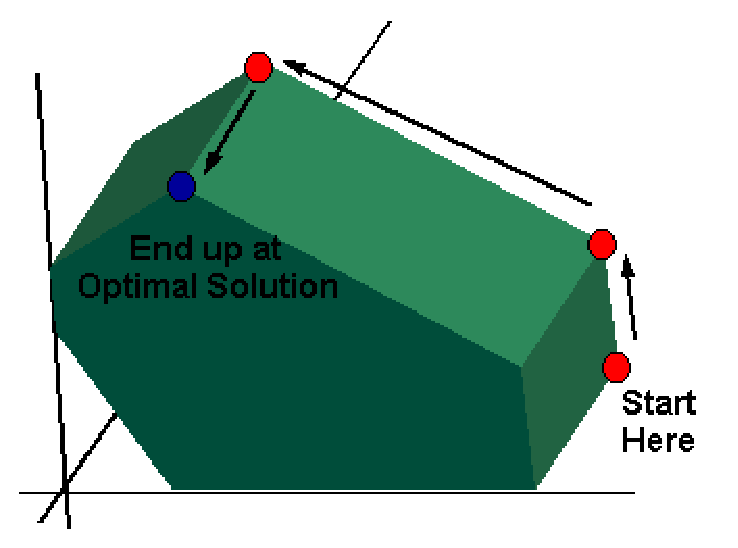
\includegraphics[width=1.7in]{L8-simplex.eps}
%\end{figure}

}


\frame{
	\frametitle{Some questions  to answer}
	\begin{enumerate}
		\item Why does it suffice to consider vertices of the polytope only?
		\item How to obtain a vertex? 
		\item How to implement ``moving to another vertex via an edge"? 
		\item When should we stop? 
	\end{enumerate}
%\begin{figure}
%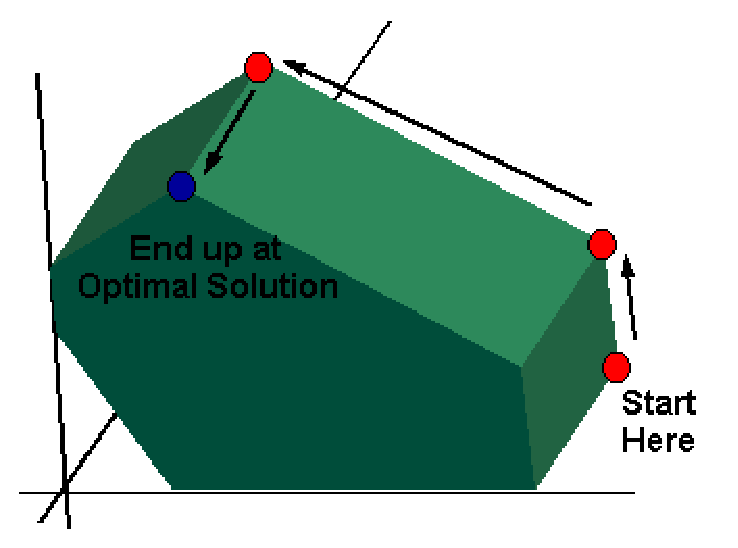
\includegraphics[width=1.7in]{L8-simplex.eps}
%\end{figure}

\begin{tikzpicture}[x=0.8cm,y=0.8cm] 
%\pgfplotsset{my style/.append style={ axis x line=middle, axis y line=middle, axis equal }}

    \begin{axis}[anchor=origin,         xlabel=$x_3$,
        ylabel=$x_4$, 
        xtick={ 0,..., 5},
        ytick={ 0,..., 5}, 
        xmin=0,
        xmax=5,
        ymin=0,
        ymax=5, 
         x=0.8cm, y=0.8cm, 
        ];
              \addplot[domain=0:4.5]{0.5*x+1};
              \addplot[domain=2:5]{1.5*x-3};
%              \addplot[domain=-1:3,-,red]{-x+1};

		
      \end{axis};
                    \node at (6,3) {$-x_3+2x_4 = 2$};
              \node at (3,4) {$3x_3-2x_4 = 6$};
%              \node[red] at (4,0) {$x_3+x_4=1$};
	\draw[fill=green!20] (0, 0) -- ( 2, 0) -- (4,3) -- (0,1) -- (0,05);
	\node[circle, minimum size=3pt,inner sep=0pt, fill=red] at (0,0) {};
		\node[circle, minimum size=3pt,inner sep=0pt, fill=red] at (2,0) {};
			\node[circle, minimum size=3pt,inner sep=0pt, fill=red] at (4,3) {};
			\node[below, red, ultra thick] at (-0.2,-0.2) {start};
			\node[below, red, ultra thick] at (4.2,3) {end};	
			\draw[->, red, ultra thick] (0,0) -- (2,0); 
			\draw[->, red, ultra thick] (2,0) -- (4,3); 
			
    \end{tikzpicture}
    
}


%\frame{
%\frametitle{Iteration: a general optimization technique}
%$Iteration(f)$
%\begin{algorithmic}[1]
%\STATE $\mathnormal{x=x}_0$; //initialization;
%\WHILE{ $TRUE$ }
%\STATE $\mathnormal{x}=improve(\mathnormal{x})$; //move a step towards optimum;
%\IF { $stopping(\mathnormal{x})$ }
%\STATE break;
%\ENDIF
%\ENDWHILE
%\RETURN $\mathnormal{x}$;
%\end{algorithmic}
%
%\begin{figure}
%\includegraphics[width=1.8in]{L8-simplex.eps}
%\end{figure}
%
%}



\frame{
\begin{block}{}
Question 1: Why  does it suffice to consider vertices of the polytope only?\\

\end{block}
\begin{figure}
 \includegraphics[width=2in] {L8-LP-GE3.png}
\end{figure}

}

\frame{
\frametitle{Optimal solution can be reached at a vertex}
\begin{Theorem}
There exists a vertex in $\mathnormal{P}$ that takes the optimal value (if the optimal objective value is finite). 
\end{Theorem}
\begin{Proof}
\begin{itemize}
\begin{footnotesize}
 \item Since $\mathnormal{P}$ is a bounded close set, $\mathnormal{c^Tx}$ reaches its optimum in $\mathnormal{P}$.
 \item Denote the optimal solution as $\mathnormal{x}^{(0)}$. We will show there is a vertex at least as good as $\mathnormal{x}^{(0)}$. Why?
\begin{itemize}
\begin{footnotesize}
 \item $\mathnormal{x}^{(0)}$ can be represented as the convex combination of vertices of $\mathnormal{P}$, i.e.  $\mathnormal{x}^{(0)} = \lambda_1 \mathnormal{x^{(1)} } + \lambda_2 \mathnormal{x^{(2)} } + ... + \lambda_{k} \mathnormal{x^{(k)} }$, where $\lambda_i \geq 0, \lambda_1 + ... + \lambda_{k} = 1 $.  (See Appendix for details.)
 \item Thus $\mathnormal{c^Tx}^{(0)} = \lambda_1 \mathnormal{ c^Tx}^{(1)} + \lambda_2 \mathnormal{ c^Tx}^{(2)} + ... + \lambda_{k} \mathnormal{ c^Tx}^{(k)}$
 \item Let $x^{(i)}$ be the vertex with the minimal objective value $\mathnormal{ c^T x}^{(i)}$;
 \item $\mathnormal{c^Tx}^{(0)} = \lambda_1 \mathnormal{ c^T x}^{(1)} + \lambda_2 \mathnormal{ c^T x}^{(2)} + ... + \lambda_{k} \mathnormal{ c^T x}^{(k)} \geq \mathnormal{ c^T x}^{(i)} $.
% \end{footnotesize}
\end{footnotesize}
\end{itemize}
 \item Thus,  vertex $\mathnormal{x}^{(i)}$ is also an optimal solution  since $\mathnormal{ c^T x}^{(i)} \leq \mathnormal{c^Tx}^{(0)}$ \end{footnotesize}
\end{itemize}
\end{Proof}
}


\frame{
\frametitle{Intuitive idea}

\begin{figure}
 \includegraphics[width=1.4in] {L8-x1x2x3.eps}
\end{figure}

\begin{itemize}
\item Suppose $\mathnormal{x}^{(0)}$ is an optimal solution. 
 \item Connecting $\mathnormal{x}^{(0)}$ and $\mathnormal{x}^{(1)}$ with a line. Suppose the line intersects line segment $(\mathnormal{x}^{(2)}, \mathnormal{x}^{(3)} )$ at point $\mathnormal{x}'$.
 \item We have $\mathnormal{x}^{(0)} = \lambda_1\mathnormal{x}^{(1)} + (1-\lambda_1) \mathnormal{x}'$, where $\lambda_1 = \frac{q}{p+q}$.
 \item We also have $\mathnormal{x}'= \lambda_2 \mathnormal{x}^{(2)} + (1-\lambda_2) \mathnormal{x}^{(3)} $, where $\lambda_2 = \frac{s}{r+s}$.
 \item Thus, we have $\mathnormal{x}^{(0)} = \lambda_1 \mathnormal{x}^{(1)} + (1-\lambda_1)\lambda_2 \mathnormal{x}^{(2)} + (1-\lambda_1)(1-\lambda_2) \mathnormal{x}^{(3)}$.
 \item Suppose $\mathnormal{ c^T x}^{(1)}$ is the minimum of $\mathnormal{c^Tx}^{(1)}, \mathnormal{c^Tx}^{(2)}, \mathnormal{c^Tx}^{(3)}$.
 \item Notice that $\lambda_1  +  (1-\lambda_1)\lambda_2 + (1-\lambda_1)(1-\lambda_2) = 1$.
  \item We have: $\mathnormal{ c^T x}^{(1)} \leq \mathnormal{ c^T x}^{(0)}$. Thus, a vertex $\mathnormal{x}^{(1)}$ is found not worse than $\mathnormal{x}^{(0)}$.
\end{itemize}

}


\frame{
\begin{block}{}
Question 2: How to obtain a vertex of the polytope? 
\end{block}
%\begin{figure}
% \includegraphics[width=1.1in] {L8-LPexample3D.eps}
%\end{figure}

\begin{figure}
\begin{tikzpicture}[scale=0.5, auto,swap]
    \coordinate (cO) at (0, 0);
    \coordinate (cX) at (3.9, -0.15);
    \coordinate (cY) at (-2.6, -2.6);
    \coordinate (cZ) at (-0.19, 5.5); 

    % 0,0,3
    \coordinate (A) at (-0.14, 4);
    % 1,0,3 
    \coordinate (B) at (1.2, 4);
    % 2,0,2 
    \coordinate (C) at (2.48, 2.4);
    % 2,0,0 
    \coordinate (D) at (2.6,-0.1);
    % 2,2,0 
    \coordinate (E) at (1.1, -1.7);
    % 0,2,0 
    \coordinate (F) at (-1.6, -1.6);
    % 0,1,3 
    \coordinate (G) at (-0.63, 3.24);

    \draw [thick, gray] (A)--(B)--(C)--(D)--(E)--(F)--(G)--cycle (B)--(G)--(E)--(C);
    \draw [dashed,thick, black] (cO)--(D) (cO)--(A) (cO)--(F);
 %   \draw [->,green, thick] (cO)->(D);
    \draw [->,color=black, thick] (D)->(cX);
    \draw [->,color=black, thick] (F)->(cY);
    \draw [->,color=black, thick] (A)->(cZ);
    
    \draw (E) node [below]{\tiny(2,2,0)};
    \draw (F) node [below right]{\tiny(0,2,0)};
    \draw (A) node [above left]{\tiny(0,0,3)};
    \draw (B) node [above]{\tiny(1,0,3)};
    \draw (G) node [above left]{\tiny(0,1,3)};
    \draw (C) node [above right]{\tiny(2,0,2)};
    \draw (D) node [below ]{\tiny(2,0,0)};
    \draw (cX) node [below]{\small $x_1$};
    \draw (cY) node [right]{\small $x_2$};
    \draw (cZ) node [right]{\small $x_3$};

 %   \draw (2.8,1.3) node [above,right,green] {\small $\lambda=[1,0,0,-1,-1,0,0]$};
 %   \draw (2.8,0.9) node [below,right,green] {\small $\theta=2$};
	
   \end{tikzpicture}
\end{figure}


}





\frame{
\frametitle{Vertex $\Leftrightarrow$ basic feasible solution}

\begin{Theorem}
A vertex of $\mathnormal{P}$ corresponds to a basis of matrix $\mathnormal{A}$.
\end{Theorem}
An example (standard form):
\begin{scriptsize}
\[
\begin{array}{rrrrrrrrrrrrl}
 \min & - x_1     &-&  14 x_2    &-& 6 x_3 \\
 s.t. &   x_1     &+&     x_2    &+& x_3 & \leq & 4   \\
      &   x_1     & &            & &     & \leq & 2   \\
      &           & &            & &  x_3& \leq & 3   \\
      &           & &   3x_2     &+&  x_3& \leq & 6   \\
      &   x_1     &,&   x_2      &,&  x_3& \geq & 0   \\
\end{array} \nonumber
\]
\end{scriptsize}
\begin{figure}
\begin{tikzpicture}[scale=0.5, auto,swap]
    \coordinate (cO) at (0, 0);
    \coordinate (cX) at (3.9, -0.15);
    \coordinate (cY) at (-2.6, -2.6);
    \coordinate (cZ) at (-0.19, 5.5); 

    % 0,0,3
    \coordinate (A) at (-0.14, 4);
    % 1,0,3 
    \coordinate (B) at (1.2, 4);
    % 2,0,2 
    \coordinate (C) at (2.48, 2.4);
    % 2,0,0 
    \coordinate (D) at (2.6,-0.1);
    % 2,2,0 
    \coordinate (E) at (1.1, -1.7);
    % 0,2,0 
    \coordinate (F) at (-1.6, -1.6);
    % 0,1,3 
    \coordinate (G) at (-0.63, 3.24);

    \draw [thick, gray] (A)--(B)--(C)--(D)--(E)--(F)--(G)--cycle (B)--(G)--(E)--(C);
    \draw [dashed,thick, black] (cO)--(D) (cO)--(A) (cO)--(F);
 %   \draw [->,green, thick] (cO)->(D);
    \draw [->,color=black, thick] (D)->(cX);
    \draw [->,color=black, thick] (F)->(cY);
    \draw [->,color=black, thick] (A)->(cZ);
    
    \draw (E) node [below]{\tiny(2,2,0)};
    \draw (F) node [below right]{\tiny(0,2,0)};
    \draw (A) node [above left]{\tiny(0,0,3)};
    \draw (B) node [above]{\tiny(1,0,3)};
    \draw (G) node [above left]{\tiny(0,1,3)};
    \draw (C) node [above right]{\tiny(2,0,2)};
    \draw (D) node [below ]{\tiny(2,0,0)};
    \draw (cX) node [below]{\small $x_1$};
    \draw (cY) node [right]{\small $x_2$};
    \draw (cZ) node [right]{\small $x_3$};

 %   \draw (2.8,1.3) node [above,right,green] {\small $\lambda=[1,0,0,-1,-1,0,0]$};
 %   \draw (2.8,0.9) node [below,right,green] {\small $\theta=2$};
	
   \end{tikzpicture}
\end{figure}

}

\frame{
\frametitle{Part 1: Vertex $\Rightarrow$ basic feasible solution}
\begin{itemize}
\item 
We will first show that \textcolor{red}{\bf any vertex} of the polytope corresponds to a basis of the matrix $\mathnormal{A}$. 
\item 
An example (slack form): 
\begin{scriptsize}
\[
\begin{array}{rrrrrrrrrrrrrrrrl}
 \min & - x_1     &-&  14 x_2    &-& 6 x_3 & &  & & & & & &\\
 s.t. &   x_1     &+&     x_2    &+& x_3  &+ & x_4 & & & & & &   			& = & 4   \\
      &   x_1     & &            & &               & &  &+ & x_5& & & & 			& = & 2   \\
      &           & &            & &  x_3	  & &  & & &+ & x_6& &			& = & 3   \\
      &           & &   3x_2     &+&  x_3	  & &  & & & & & +&x_7			& = & 6   \\
      &   x_1     &,&   x_2      &,&  x_3    &, & x_4 &, &x_5 &, & x_6& ,&	x_7	        & \geq & 0   \\
\end{array} \nonumber
\]
\end{scriptsize}
\begin{figure}
\begin{tikzpicture}[scale=0.5, auto,swap]
    \coordinate (cO) at (0, 0);
    \coordinate (cX) at (3.9, -0.15);
    \coordinate (cY) at (-2.6, -2.6);
    \coordinate (cZ) at (-0.19, 5.5); 

    % 0,0,3
    \coordinate (A) at (-0.14, 4);
    % 1,0,3 
    \coordinate (B) at (1.2, 4);
    % 2,0,2 
    \coordinate (C) at (2.48, 2.4);
    % 2,0,0 
    \coordinate (D) at (2.6,-0.1);
    % 2,2,0 
    \coordinate (E) at (1.1, -1.7);
    % 0,2,0 
    \coordinate (F) at (-1.6, -1.6);
    % 0,1,3 
    \coordinate (G) at (-0.63, 3.24);

    \draw [thick, gray] (A)--(B)--(C)--(D)--(E)--(F)--(G)--cycle (B)--(G)--(E)--(C);
    \draw [dashed,thick, black] (cO)--(D) (cO)--(A) (cO)--(F);
 %   \draw [->,green, thick] (cO)->(D);
    \draw [->,color=black, thick] (D)->(cX);
    \draw [->,color=black, thick] (F)->(cY);
    \draw [->,color=black, thick] (A)->(cZ);
    
    \draw (E) node [below]{\tiny(2,2,0)};
    \draw (F) node [below right]{\tiny(0,2,0)};
    \draw (A) node [above left]{\tiny(0,0,3)};
    \draw (B) node [above]{\tiny(1,0,3)};
    \draw (G) node [above left]{\tiny(0,1,3)};
    \draw (C) node [above right]{\tiny(2,0,2)};
    \draw (D) node [below ]{\tiny(2,0,0)};
    \draw (cX) node [below]{\small $x_1$};
    \draw (cY) node [right]{\small $x_2$};
    \draw (cZ) node [right]{\small $x_3$};

 %   \draw (2.8,1.3) node [above,right,green] {\small $\lambda=[1,0,0,-1,-1,0,0]$};
 %   \draw (2.8,0.9) node [below,right,green] {\small $\theta=2$};
	
   \end{tikzpicture}
\end{figure}

\end{itemize}
}




%\frame{
%\frametitle{}
%\begin{itemize}
%  \item
% Consider a LP model with constraints as follows:
%\begin{scriptsize}
% \[
% \begin{array}{rrrrrrrrrrrrl}
%    & a_{11}x_1 &+& a_{12}x_2 &+& ... &+& a_{1n}x_n & = & b_1 &  \\
%   & a_{21}x_1 &+& a_{22}x_2 &+& ... &+& a_{2n}x_n & = & b_2 &  \\
%    &           & &           & & ... & &           &      &     &  \\
%    & a_{m1}x_1 &+& a_{m2}x_2 &+& ... &+& a_{mn}x_n & = & b_m &  \\
%    & x_1 &,& x_2 &,& ... &,& x_n & \geq & 0 &  \\
% \end{array} \nonumber
% \]
%  \end{scriptsize}
%\item
%Applying Gaussian elimination, we have:
%\begin{scriptsize}
%\[
%\begin{array}{rrrrrrrrrrrrrrrrrl}
%   & x_1 & &     & &     &+& a_{1,m+1}'x_{m+1} &+& ... &+& a_{1n}'x_n & = & b_1' &  \\
%   &     & & x_2 & &     &+& a_{2,m+1}'x_{m+1} &+&... &+& a_{2n}'x_n & = & b_2' &  \\
%   &     & &  ...& &     & & ... & &           &      &     &  \\
%   &     & &     & & x_m &+& a_{m,m+1}'x_{m+1}&+&... &+& a_{mn}'x_n & = & b_m' &  \\
%   & x_1 &,& x_2 &,& x_m &,& x_{m+1}&,&... &,& x_n & \geq & 0 &  \\
%\end{array} \nonumber
%\]
%\end{scriptsize}
%\item
%Define polytope $P \subset \mathnormal{R}^{n-m}$ as the intersection of $m$ half-spaces:
%$HS_j: a_{j,m+1}'x_{m+1} + ... + a_{jn}'x_n  \leq  b_j' $, $1\leq j \leq m$.
%\item We will show that any vertex of $P$ corresponds to a basic feasible solution of the LP model.
%\end{itemize}
%}


\frame[allowframebreaks]{
\frametitle{Intuitive idea  }


% \begin{figure}%
%   \begin{center}%
%     \begin{minipage}{0.25\textwidth}%
%      \includegraphics[width=1.0\textwidth]{L8-LPexample3Dvertex.eps}%
%     \end{minipage}%
%     \quad
%     \begin{minipage}{0.32\textwidth}
%      \includegraphics[width=1.0\textwidth]{L8-LPexample3Dvertexmatrix.png}%
%     \end{minipage}%
%   \end{center}
% \end{figure}


\begin{figure}
\begin{tikzpicture}[scale=0.7, auto,swap]
    \coordinate (cO) at (0, 0);
    \coordinate (cX) at (3.9, -0.15);
    \coordinate (cY) at (-2.2, -2.2);
    \coordinate (cZ) at (-0.17, 5.0); 

    % 0,0,3
    \coordinate (A) at (-0.14, 4);
    % 1,0,3 
    \coordinate (B) at (1.2, 4);
    % 2,0,2 
    \coordinate (C) at (2.48, 2.4);
    % 2,0,0 
    \coordinate (D) at (2.6,-0.1);
    % 2,2,0 
    \coordinate (E) at (1.1, -1.7);
    % 0,2,0 
    \coordinate (F) at (-1.6, -1.6);
    % 0,1,3 
    \coordinate (G) at (-0.63, 3.24);
    
        \coordinate (x1) at (-2.1, -1.1);
            \coordinate (x2) at (-1.1, -2.1);

    \draw [thick, gray] (A)--(B)--(C)--(D)--(E)--(F)--(G)--cycle (B)--(G)--(E)--(C);
    \draw [dashed,thick, black] (cO)--(D) (cO)--(A) (cO)--(F);
%    \draw [->,green, thick] (cO)->(D);
    \draw [->,color=black, thick] (D)->(cX);
    \draw [->,color=black, thick] (F)->(cY);
    \draw [->,color=black, thick] (A)->(cZ);
    
    \draw (E) node [below]{\tiny(2,2,0)};
    \draw (F) node [red, above right, thick]{\tiny $\mathnormal{x}=\left[ 0\ 2\ 0\  2\ 2\ 3\ 0 \right]^T$};
    \draw (A) node [above left]{\tiny(0,0,3)};
    \draw (B) node [above]{\tiny(1,0,3)};
    \draw (G) node [above left]{\tiny(0,1,3)};
    \draw (C) node [above right]{\tiny(2,0,2)};
    \draw (D) node [below right]{\tiny(2,0,0)};
    \draw (cX) node [below]{\small $x_1$};
    \draw (cY) node [right]{\small $x_2$};
    \draw (cZ) node [right]{\small $x_3$};

   \draw [->, thick, green] (x2) -- (x1);
   \draw [fill=red, draw=white]  (F)  circle(2pt); 
   \draw [fill=green, draw=white]  (x1)  circle(2pt); 
   \draw [fill=green, draw=white]  (x2)  circle(2pt); 
   
   \draw (x1) node [above, left, green, thick] {\tiny $\mathnormal{x'=x+\lambda}$};
      \draw (x2) node [below, right, green, thick] {\tiny $\mathnormal{x''=x-\lambda}$};
%    \draw (2.8,1.3) node [above,right,green] {\small $\lambda=[1,0,0,-1,-1,0,0]$};
%    \draw (2.8,0.9) node [below,right,green] {\small $\theta=2$};
    
            \draw (3.4, 3.5) node [above,right] {\tiny $
 \mathnormal{x}=\left[ \begin{array}{ccccccc}
0 & \textcolor{blue}{2} & 0 & \textcolor{blue}{2} & \textcolor{blue}{2}  & \textcolor{blue}{3}  & 0 
 \end{array} \right]
^T$};	
        \draw (3.3, 2.5) node [above,right] {\tiny $
 \mathnormal{A}=\left[ \begin{array}{ccccccc}
1 & \textcolor{blue}{1} & 1 & \textcolor{blue}{1} & \textcolor{blue}{0}  & \textcolor{blue}{0}  & 0 \\
1 & \textcolor{blue}{0} & 0 & \textcolor{blue}{0} & \textcolor{blue}{1}  & \textcolor{blue}{0}  & 0 \\
0 & \textcolor{blue}{0} & 1 & \textcolor{blue}{0} & \textcolor{blue}{0}  & \textcolor{blue}{1}  & 0 \\
0 & \textcolor{blue}{3} & 1 & \textcolor{blue}{0} & \textcolor{blue}{0}  & \textcolor{blue}{0}  & 1\\
 \end{array} \right]
$};		
   \end{tikzpicture}
\end{figure}


\begin{scriptsize}

%\begin{tiny}
%\begin{table}
%{
%\begin{tabular}{rrrrrrrr}
%  \textcolor{blue}{$x_1$} & \textcolor{blue}{$x_2$} & $x_3$ & $x_4$ & $x_5$ & \textcolor{blue}{$x_6$} & {$x_7$}\\
%\hline
%% -z= 30 & $\overline{c_1}$= 0 & $\overline{c_2}$=0 & $\overline{c_3}$=8 & $\overline{c_4}$=14 & $\overline{c_5}$=-13 & $\overline{c_6}$=0 & $\overline{c_7}$=0 \\
% %\hline
% \textcolor{blue}{0} & \textcolor{blue}{1} & 1 & 1 & -1& \textcolor{blue}{0} & {0} \\
% \textcolor{blue}{1} & \textcolor{blue}{0} & 0 & 0 & 1 & \textcolor{blue}{0} & {0} \\
% \textcolor{blue}{0} & \textcolor{blue}{0} & 1 & 0 & 0 & \textcolor{blue}{1} & {0} \\
% \textcolor{blue}{0} & \textcolor{blue}{0} &-2 &-3 & 3 & \textcolor{blue}{0} & {1} \\
%\hline
%\end{tabular}
%} %{}%
%\end{table}
%\end{tiny}
\begin{itemize}
 \item Take the vertex $(x_1, x_2, x_3) = (0,2,0)$ as an example. The corresponding full solution is $(x_1,x_2,x_3,x_4,x_5,x_6,x_7)= ( 0, 2, 0, 2, 2, 3, 0)$. 
  \item We will show that the column vectors corresponding to \textcolor{blue}{\bf non-zero $x_i$}, i.e. $\mathnormal{ \textcolor{blue}{ \{a_2, a_4, a_5, a_6 \}}}$, are linearly independent, and thus form a basis (sometimes an extension is needed). (Here  $\mathnormal{a_i}$ denotes the $i$-th column vector of $\mathnormal{A}$)
  \item Suppose $\exists (\lambda_2, \lambda_4, \lambda_5,\lambda_6) \neq 0$ such that $\lambda_{2}\textcolor{blue}{\mathnormal{a_{2}}} + \lambda_{4}\textcolor{blue}{\mathnormal{a_{4}}} + \lambda_{5}\textcolor{blue}{\mathnormal{a_{5}}}+ \lambda_{6}\textcolor{blue}{\mathnormal{a_{6}}}  = 0$, i.e. $\mathnormal{A\lambda=}0$, where $\mathnormal{\lambda} = [0, \lambda_2, 0, \lambda_4, \lambda_5,\lambda_6, 0]$.
  \item Then we can construct \textcolor{green}{\bf two other points: $\mathnormal{x'=x+\theta \lambda}$ and $\mathnormal{x''=x-\theta \lambda}$. }

  
  \begin{figure}
\begin{tikzpicture}[scale=0.7, auto,swap]
    \coordinate (cO) at (0, 0);
    \coordinate (cX) at (3.9, -0.15);
    \coordinate (cY) at (-2.2, -2.2);
    \coordinate (cZ) at (-0.17, 5.0); 

    % 0,0,3
    \coordinate (A) at (-0.14, 4);
    % 1,0,3 
    \coordinate (B) at (1.2, 4);
    % 2,0,2 
    \coordinate (C) at (2.48, 2.4);
    % 2,0,0 
    \coordinate (D) at (2.6,-0.1);
    % 2,2,0 
    \coordinate (E) at (1.1, -1.7);
    % 0,2,0 
    \coordinate (F) at (-1.6, -1.6);
    % 0,1,3 
    \coordinate (G) at (-0.63, 3.24);
    
        \coordinate (x1) at (-2.1, -1.1);
            \coordinate (x2) at (-1.1, -2.1);

    \draw [thick, gray] (A)--(B)--(C)--(D)--(E)--(F)--(G)--cycle (B)--(G)--(E)--(C);
    \draw [dashed,thick, black] (cO)--(D) (cO)--(A) (cO)--(F);
%    \draw [->,green, thick] (cO)->(D);
    \draw [->,color=black, thick] (D)->(cX);
    \draw [->,color=black, thick] (F)->(cY);
    \draw [->,color=black, thick] (A)->(cZ);
    
    \draw (E) node [below]{\tiny(2,2,0)};
    \draw (F) node [red, above right, thick]{\tiny $\mathnormal{x}=\left[ 0\ 2\ 0\  2\ 2\ 3\ 0 \right]^T$};
    \draw (A) node [above left]{\tiny(0,0,3)};
    \draw (B) node [above]{\tiny(1,0,3)};
    \draw (G) node [above left]{\tiny(0,1,3)};
    \draw (C) node [above right]{\tiny(2,0,2)};
    \draw (D) node [below right]{\tiny(2,0,0)};
    \draw (cX) node [below]{\small $x_1$};
    \draw (cY) node [right]{\small $x_2$};
    \draw (cZ) node [right]{\small $x_3$};

   \draw [->, thick, green] (x2) -- (x1);
   \draw [fill=red, draw=white]  (F)  circle(2pt); 
   \draw [fill=green, draw=white]  (x1)  circle(2pt); 
   \draw [fill=green, draw=white]  (x2)  circle(2pt); 
   
   \draw (x1) node [above, left, green, thick] {\tiny $\mathnormal{x'=x+\lambda}$};
      \draw (x2) node [below, right, green, thick] {\tiny $\mathnormal{x''=x-\lambda}$};
%    \draw (2.8,1.3) node [above,right,green] {\small $\lambda=[1,0,0,-1,-1,0,0]$};
%    \draw (2.8,0.9) node [below,right,green] {\small $\theta=2$};
    
            \draw (3.4, 3.5) node [above,right] {\tiny $
 \mathnormal{x}=\left[ \begin{array}{ccccccc}
0 & \textcolor{blue}{2} & 0 & \textcolor{blue}{2} & \textcolor{blue}{2}  & \textcolor{blue}{3}  & 0 
 \end{array} \right]
^T$};	
        \draw (3.3, 2.5) node [above,right] {\tiny $
 \mathnormal{A}=\left[ \begin{array}{ccccccc}
1 & \textcolor{blue}{1} & 1 & \textcolor{blue}{1} & \textcolor{blue}{0}  & \textcolor{blue}{0}  & 0 \\
1 & \textcolor{blue}{0} & 0 & \textcolor{blue}{0} & \textcolor{blue}{1}  & \textcolor{blue}{0}  & 0 \\
0 & \textcolor{blue}{0} & 1 & \textcolor{blue}{0} & \textcolor{blue}{0}  & \textcolor{blue}{1}  & 0 \\
0 & \textcolor{blue}{3} & 1 & \textcolor{blue}{0} & \textcolor{blue}{0}  & \textcolor{blue}{0}  & 1\\
 \end{array} \right]
$};		
   \end{tikzpicture}
\end{figure}

\item It is easy to deduce  that both $\mathnormal{x'}$ and $\mathnormal{x''}$ lie inside $P$ since: 

\begin{itemize}
\begin{scriptsize}
\item $\mathnormal{A x' = Ax +} 0 = \mathnormal{ b}$ and   $\mathnormal{A x'' = Ax -}  0 = \mathnormal{b}$
\item In addition, we can guarantee $\mathnormal{x'} \geq 0$ and  $\mathnormal{x''} \geq 0$ via setting $\theta$ to be sufficiently small since $\mathnormal{x \geq} 0$, and $\lambda_1=\lambda_3=\lambda_7=0$.
\end{scriptsize}
\end{itemize}
 \item Contradiction: it is impossible for a vertex to be  middle point of two inner points of $\mathnormal{P}$. 
 \end{itemize}
\end{scriptsize}


}

%\frame{
%
%$
%\mathnormal{x}= \ \left[ \begin{array}{ccccccc}
%               0 &\textcolor{blue}{2} &0 &\textcolor{blue}{2} &\textcolor{blue}{2} &\textcolor{blue}{3} &0 
%               \end{array}
%               \right]^T
%$\\
%$\mathnormal{A}=\left[ 
%		\begin{array}{ccccccc}
%		1 & \textcolor{blue}{1} & 1 & \textcolor{blue}{1} & \textcolor{blue}{0} & \textcolor{blue}{0} & 0 \\
%		1 & \textcolor{blue}{0} & 0 & \textcolor{blue}{0} & \textcolor{blue}{1} & \textcolor{blue}{0} & 0 \\
%		0 & \textcolor{blue}{0} & 1 & \textcolor{blue}{0} & \textcolor{blue}{0} & \textcolor{blue}{1} & 0 \\
%		0 & \textcolor{blue}{3} & 1 & \textcolor{blue}{0} & \textcolor{blue}{0} & \textcolor{blue}{0} & 1 
%		\end{array}
%		\right] 
%		\mathnormal{b} = \left[ \begin{array}{c} 
%						4\\
%						2\\
%						3\\
%						6
%					 	\end{array} \right]
%$\\
%$ \mathnormal{B} = \left[ 
%			\begin{array}{cccc}
%		 \textcolor{blue}{1} &  \textcolor{blue}{1} & \textcolor{blue}{0} & \textcolor{blue}{0}  \\
%		 \textcolor{blue}{0} &  \textcolor{blue}{0} & \textcolor{blue}{1} & \textcolor{blue}{0}  \\
%		 \textcolor{blue}{0} &  \textcolor{blue}{0} & \textcolor{blue}{0} & \textcolor{blue}{1}  \\
%		 \textcolor{blue}{3} &  \textcolor{blue}{0} & \textcolor{blue}{0} & \textcolor{blue}{0}  				
%			\end{array}
%			\right]  \mathnormal{N}= \left[
%			\begin{array}{ccc}
%			1 & 1 & 0 \\
%			1 & 0 & 0 \\
%			0 & 1 & 0 \\
%			0 & 1 & 1 
%			\end{array}
%			\right]
%			$\\
%$ \mathnormal{x_B}=[2\ 2\ 2\ 3]^T =  \mathnormal{B^{-1}b} $
%
%}


\frame{
\frametitle{Proof}
\begin{footnotesize}
\begin{enumerate}
\begin{scriptsize}
 \item
Suppose $\mathnormal{ \hat{x} } =<x_{m+1}, ..., x_n>$ is a vertex of $\mathnormal{P} \subset \mathbb{R}^{n-m}$, i.e.  we have $ a'_{i, m+1} x_{m+1} + ... + a'_{i,n} x_n \leq b'_i $ for all $1 \leq i \leq m$.
\item
Expanding \textcolor{red}{partial} solution $\mathnormal{ \hat{x} }$ to a feasible \textcolor{red}{full} solution $\mathnormal{x}=<x_1,..., x_m, x_{m+1}, ..., x_n>$, where $x_1,...,x_m$ are calculated according to  the equality constraints of the LP model.
\item Considering the non-zero items $x_j$ in $\mathnormal{x}$. Note that the corresponding columns $\mathnormal{B=\{a}_j | x_j \neq 0\} $ form a basis. Why?
\begin{enumerate}
\begin{scriptsize}
\item
Suppose there exist $d_j$ such that $ \sum_{  \mathnormal{a}_j \in \mathnormal{B} } d_j  \mathnormal{a}_j = {0}$ ( $<d_j>\neq 0$).
\item
Since $\sum_{ \mathnormal{a}_j \in \mathnormal{B}} x_j  \mathnormal{a}_j = \mathnormal{b} $ ( $x_k=0$ for all  $  \mathnormal{a}_k\notin \mathnormal{B} $ ),  we can construct two \textcolor{red}{full} feasible solutions $<x_i + \theta d_i>$ and $<x_i - \theta d_i>$ since:

$\sum_{ \mathnormal{a}_j \in \mathnormal{B} } (x_j \pm \theta d_j)  \mathnormal{a}_j = \mathnormal{b} $. (We can guarantee $ x_j \pm \theta d_j \geq 0$ through setting $\theta$ sufficiently small.)

 \item Thus the corresponding two \textcolor{red}{partial} solutions are in $\mathnormal{P}$:
$\mathnormal{x}'=<x_{m+1}', ..., x_n'>$, where $x_j' = x_j + \theta d_j$ for $ \mathnormal{a}_j \in \mathnormal{B}$, and 0 otherwise; \\
$\mathnormal{x}''=<x_{m+1}'', ..., x_n''>$, where $x_j'' = x_j - \theta d_j$ for $ \mathnormal{a}_j \in \mathnormal{B}$, and 0 otherwise;\\
 \item
Thus $\mathnormal{\hat{x}} = \frac{1}{2} \mathnormal{x}' + \frac{1}{2} \mathnormal{x}''$. A contradiction. (A vertex in $P$ cannot be represented as the convex combination of two points in $P$. See Appendix.)
\end{scriptsize}
\end{enumerate}
\item
Thus, $\mathnormal{x}$ is a basic feasible solution corresponding to basis $\mathnormal{B}$ since:  1) $\mathnormal{x}$ can be represented as $\mathnormal{x=\left[\begin{array}{c}\mathnormal{x_B}\\{0}\end{array}\right]}$, and 2) any item $x_j \geq 0$. $\qed$
\end{scriptsize}
\end{enumerate}
\end{footnotesize}

}



\frame{
\frametitle{Vertex $\Rightarrow$  basic feasible  solution: some notations  }
\begin{itemize}
\item For a vertex $\mathnormal{x}$ of the polytope, a basis $\mathnormal{B}$ can be derived via extracting the column vectors corresponding to non-zero $x_i$. The non-basis column vectors are denoted as $\mathnormal{N}$.
\item Then  the original LP  can be represented as:
\begin{figure}
 \includegraphics[width=2.5in] {L8-simplextable.png}
\end{figure}
 \item Here, $\mathnormal{x}$  is decomposed as $\mathnormal{x=\left[\begin{array}{c}\mathnormal{x_B}\\\mathnormal{x_N}\end{array}\right]}$. Then  we have $\mathnormal{x_N=0}$, and $\mathnormal{x_B=B^{-1}b}$ (Reason: $\mathnormal{Ax=b}$, i.e. $\mathnormal{B x_B + N x_N = b}$ )
 \item The corresponding objective value is $\mathnormal{c^T x = c_B^T x_B + c_N^T x_N = c_B^T B^{-1} b }$.
 \end{itemize}
 }
 
\frame{
\frametitle{An example  }
 \begin{itemize}
 \item For a vertex $\mathnormal{x}= \ \left[ \begin{array}{ccccccc}
               0 &\textcolor{blue}{2} &0 &\textcolor{blue}{2} &\textcolor{blue}{2} &\textcolor{blue}{3} &0 
               \end{array}
               \right]^T$, the columns corresponding to non-zero $x_i$ are extracted to form a basis 
$ \mathnormal{B} = \left[ 
			\begin{array}{cccc}
		 \textcolor{blue}{1} &  \textcolor{blue}{1} & \textcolor{blue}{0} & \textcolor{blue}{0}  \\
		 \textcolor{blue}{0} &  \textcolor{blue}{0} & \textcolor{blue}{1} & \textcolor{blue}{0}  \\
		 \textcolor{blue}{0} &  \textcolor{blue}{0} & \textcolor{blue}{0} & \textcolor{blue}{1}  \\
		 \textcolor{blue}{3} &  \textcolor{blue}{0} & \textcolor{blue}{0} & \textcolor{blue}{0}  				
			\end{array}
			\right]$. 
\item Let's decompose $\mathnormal{x}= \ \left[ \begin{array}{ccccccc}
               0 &\textcolor{blue}{2} &0 &\textcolor{blue}{2} &\textcolor{blue}{2} &\textcolor{blue}{3} &0 
               \end{array}
               \right]^T
$ accordingly into  $ \mathnormal{x_B}=[\textcolor{blue}{2\ 2\ 2\ 3}]^T$\text{ and }  $\mathnormal{x_N}=[0\ 0\ 0]^T$.
\item It is easy to verify that $\mathnormal{x_B = B^{-1}b}$. In this example, $\mathnormal{b} = \left[ \begin{array}{c} 
						4\\
						2\\
						3\\
						6
					 	\end{array} \right]$.
						
 \end{itemize}
}

\frame{
\frametitle{Part 2: Basic feasible  solution  $\Rightarrow$ vertex  } 
\begin{itemize}
\item Given a  basis $\mathnormal{B}$ of matrix $\mathnormal{A}$,  we call $\mathnormal{x=\left[\begin{array}{c}\mathnormal{B^{-1}b}\\{0}\end{array}\right]}$ a  \textcolor{red}{\bf basic solution respect to $\mathnormal{B}$}.
 \item If we further have $\mathnormal{x_B = B^{-1}b} \geq 0$, $\mathnormal{x}$ is called  a \textcolor{red}{\bf basic feasible solution respect to $\mathnormal{B}$}.
 \item We will show that a \textcolor{red}{\bf basic feasible solution $\mathnormal{x}$ respect to $\mathnormal{B}$} is a vertex of the polytope $\mathnormal{P}$. 
  \end{itemize} 
 \begin{proof}
\begin{itemize}
\begin{small}
 \item It suffices to show that $\mathnormal{x}$ cannot be represented as a convex combination of any two points in $\mathnormal{P}$.
\item By contradiction, suppose there are two different points $\mathnormal{x}^{(1)}$ and $\mathnormal{x}^{(2)}$ in $\mathnormal{P}$ such that $\mathnormal{x} = \lambda_1 \mathnormal{x}^{(1)} + \lambda_2 \mathnormal{x}^{(2)}$, where $0 < \lambda_1, \lambda_2 < 1$. 
\item Note that $\lambda_1 \mathnormal{x}^{(1)}_N + \lambda_2 \mathnormal{x}^{(2)}_N = \mathnormal{x_N} = 0$. 
\item So $\mathnormal{x}^{(1)}_N = \mathnormal{x}^{(2)}_N = 0$ (by $\lambda_1, \lambda_2 \geq 0$ and $\mathnormal{x}^{(1)}_N, \mathnormal{x}^{(2)}_N \geq 0$). 
\item Then we have  $\mathnormal{x}^{(1)}_B = \mathnormal{x}^{(2)}_B = \mathnormal{B^{-1}b} = \mathnormal{x_B}$ (by $\mathnormal{Ax}^{(1)}=\mathnormal{b}$ and  $\mathnormal{Ax}^{(2)}=\mathnormal{b}$). A contradiction.  
\end{small}
 \end{itemize} 
 \end{proof}

} 

\frame{
\frametitle{An example }  
\begin{itemize} 
\item 
For matrix $\mathnormal{A}=\left[ 
		\begin{array}{ccccccc}
		1 & \textcolor{blue}{1} & 1 & \textcolor{blue}{1} & \textcolor{blue}{0} & \textcolor{blue}{0} & 0 \\
		1 & \textcolor{blue}{0} & 0 & \textcolor{blue}{0} & \textcolor{blue}{1} & \textcolor{blue}{0} & 0 \\
		0 & \textcolor{blue}{0} & 1 & \textcolor{blue}{0} & \textcolor{blue}{0} & \textcolor{blue}{1} & 0 \\
		0 & \textcolor{blue}{3} & 1 & \textcolor{blue}{0} & \textcolor{blue}{0} & \textcolor{blue}{0} & 1 
		\end{array}
		\right],  
		 \text{ and } \mathnormal{b} = \left[ \begin{array}{c} 
						4\\
						2\\
						3\\
						6
					 	\end{array} \right]
$, we first calculate a basis of $\mathnormal{A}$ as 
 $\mathnormal{B} = \left[ 
			\begin{array}{cccc}
		 \textcolor{blue}{1} &  \textcolor{blue}{1} & \textcolor{blue}{0} & \textcolor{blue}{0}  \\
		 \textcolor{blue}{0} &  \textcolor{blue}{0} & \textcolor{blue}{1} & \textcolor{blue}{0}  \\
		 \textcolor{blue}{0} &  \textcolor{blue}{0} & \textcolor{blue}{0} & \textcolor{blue}{1}  \\
		 \textcolor{blue}{3} &  \textcolor{blue}{0} & \textcolor{blue}{0} & \textcolor{blue}{0}  				
			\end{array}
			\right]$. 
%			
%			$  \mathnormal{N}= \left[
%			\begin{array}{ccc}
%			1 & 1 & 0 \\
%			1 & 0 & 0 \\
%			0 & 1 & 0 \\
%			0 & 1 & 1 
%			\end{array}
%			\right],
%			$\\
%\ \\
\item 
The  \textcolor{red}{\bf basic feasible solution $\mathnormal{x}$ respect to $\mathnormal{B}$} is   $\mathnormal{x=\left[\begin{array}{c}\mathnormal{B^{-1}b}\\{0}\end{array}\right]} = \ \left[ \begin{array}{ccccccc}
               0 &\textcolor{blue}{2} &0 &\textcolor{blue}{2} &\textcolor{blue}{2} &\textcolor{blue}{3} &0 
               \end{array}
               \right]^T
$. 
\item 
It is easy to verify  that $(x_1, x_2, x_3) = (0, 2, 0)$ is a vertex of the polytope $\mathnormal{P}$. 
\end{itemize} 

}


% \frame{
% $\Leftarrow$: \\
%
% Suppose $x=<x_1,..., x_m, x_{m+1}, ..., x_n>$ is a feasible basis solution, i.e.  $\exist \mathnormal{B}$, $x=<x_B, x_{\overline{B}}>$.
%
% Set $c_j = 1$ iff $ \mathnormal{a}_j \in \mathnormal{B}$. $x$ is the optimal solution of:
%
%
%
% }

\frame{
\begin{block}{}
 Question 3: How to implement ``moving from a vertex to another vertex via an edge"? 
 \end{block}
\begin{figure}
 \includegraphics[width=2in] {L8-LPexample3Dstep2.eps}
\end{figure}

}


\frame{
\frametitle{Edge $\Leftrightarrow$ non-basis column vector of $\mathnormal{A}$: an example }

 \begin{figure}%
   \begin{center}%
     \begin{minipage}{0.43\textwidth}%
      \includegraphics[width=1.0\textwidth]{L8-LPexample3Dstep2.eps}%
     \end{minipage}%
     \quad
     \begin{minipage}{0.43\textwidth}
      \includegraphics[width=1.0\textwidth]{L8-LPexample3Dedgematrix.png}%
     \end{minipage}%
   \end{center}
 \end{figure}

%\begin{figure}
% \includegraphics[width=1.6in] {L8-LPexample3Dstep2.eps}
%\end{figure}

\begin{scriptsize}
%\begin{table}
%{
%\begin{tabular}{r|rrrrrrr}
%  & \textcolor{blue}{$x_1$} & $x_2$ & $x_3$ & \textcolor{blue}{$x_4$} & $x_5$ & \textcolor{blue}{$x_6$} & \textcolor{blue}{$x_7$}\\
%\hline
% -z= 2 & $\overline{c_1}$= 0 & $\overline{c_2}$=-14 & $\overline{c_3}$=-6 & $\overline{c_4}$=0 & $\overline{c_5}$=1 & $\overline{c_6}$=0 & $\overline{c_7}$=0 \\
% \hline
% $\mathnormal{x_{B1}} = b_1'$=2 & \textcolor{blue}{0} & 1 & \textcolor{green}{1} & \textcolor{blue}{1} & -1 & \textcolor{blue}{0} & \textcolor{blue}{0} \\
% $\mathnormal{x_{B2}} = b_2'$=2 & \textcolor{blue}{1} & 0 &  \textcolor{green}{0} & \textcolor{blue}{0} & 1 & \textcolor{blue}{0} & \textcolor{blue}{0} \\
% $\mathnormal{x_{B3}} = b_3'$=3 & \textcolor{blue}{0} & 0 & \textcolor{green}{1} & \textcolor{blue}{0} & 0 & \textcolor{blue}{1} & \textcolor{blue}{0} \\
% $\mathnormal{x_{B4}} = b_4'$=6 & \textcolor{blue}{0} & 3 &  \textcolor{green}{1} & \textcolor{blue}{0} & 0 & \textcolor{blue}{0} & \textcolor{blue}{1} \\
%\hline
%\end{tabular}
%} %{}%
%\end{table}

\begin{itemize}
 \item Take the vertex  $(x_1,x_2,x_3)=(2,0,0)$ as an example. The corresponding full solution is $(x_1,x_2,x_3,x_4,x_5,x_6,x_7) = ( 2, 0, 0, 2, 0, 3, 6 )$.
  \item Basis (in blue): $\mathnormal{B =\{ \textcolor{blue}{a_1, a_4, a_6, a_7} \} }$. 
 \item  Let's consider a \textcolor{green}{\bf non-basis column vector} $\mathnormal{\textcolor{green}{a_{3}}}$. 
 \item  Since $\mathnormal{a_3}$ can be decomposed as  $\mathnormal{\textcolor{green}{a_{3}} = \textcolor{blue}{1 a_{4} + 0 a_{1} + 1 a_{6} + 1 a_{7}}}$,  we have $\mathnormal{ 0 a_{1} + 0 a_{2} - 1 a_{3} + 1 a_{4} + 0 a_{5} + 1a_{6} + 1a_{7} = 0}$
  \item We will show that the coefficients   $\textcolor{green} {\mathnormal{\lambda}= [0, 0, -1, 1, 0, 1, 1 ]^T}$ specifies the direction of  \textcolor{green}{\bf the  edge in green}. 
  \item More specifically, we can move via the edge to another vertex $\mathnormal{x'=x - \theta \lambda} = [ 2,0,2,0,0,1,4]^T$ (by setting $\theta=2$).
  \item The new vertex corresponds to  the basis  $\mathnormal{B' = B-\{\textcolor{blue}{a_4}\} \cup \{\textcolor{green}{a_3}\} =\{ \textcolor{blue}{a_1, } \textcolor{green}{a_3}, \textcolor{blue}{ a_6, a_7} \}}$. 
\end{itemize}
\end{scriptsize}
}



%\frame{
%
%$
%\mathnormal{x}= \ \left[ \begin{array}{ccccccc}
%               0 & \textcolor{blue}{2} &0 & \textcolor{blue}{2} & \textcolor{blue}{2} &  \textcolor{blue}{3} &0 
%               \end{array}
%               \right]^T
%$\\
%$\mathnormal{A}=\left[ 
%		\begin{array}{ccccccc}
%	 	\textcolor{black}{1} & \textcolor{blue}{1} & \textcolor{black}{1} & \textcolor{blue}{1} & \textcolor{blue}{0} & \textcolor{blue}{0} & \textcolor{black}{0} \\
%		\textcolor{black}{1} & \textcolor{blue}{0} & \textcolor{black}{0} & \textcolor{blue}{0} & \textcolor{blue}{1} & \textcolor{blue}{0} & \textcolor{black}{0} \\
%		\textcolor{black}{0} & \textcolor{blue}{0} & \textcolor{black}{1} & \textcolor{blue}{0} & \textcolor{blue}{0} & \textcolor{blue}{1} & \textcolor{black}{0} \\
%		\textcolor{black}{0} & \textcolor{blue}{3} & \textcolor{black}{1} & \textcolor{blue}{0} & \textcolor{blue}{0} & \textcolor{blue}{0} & \textcolor{black}{1} 
%		\end{array}
%		\right]
%$
%}
%
%
%
%\frame{
%
%$
%\mathnormal{x}= \ \left[ \begin{array}{ccccccc}
%               \textcolor{blue}{2} &0 &0 &\textcolor{blue}{2} &0 & \textcolor{blue}{3} &\textcolor{blue}{6} 
%               \end{array}
%               \right]^T
%$\\
%$\mathnormal{A}=\left[ 
%		\begin{array}{ccccccc}
%	 	\textcolor{blue}{1} & 1 & \textcolor{green}{1} & \textcolor{blue}{1} & 0 & \textcolor{blue}{0} & \textcolor{blue}{0} \\
%		\textcolor{blue}{1} & 0 & \textcolor{green}{0} & \textcolor{blue}{0} & 1 & \textcolor{blue}{0} & \textcolor{blue}{0} \\
%		\textcolor{blue}{0} & 0 & \textcolor{green}{1} & \textcolor{blue}{0} & 0 & \textcolor{blue}{1} & \textcolor{blue}{0} \\
%		\textcolor{blue}{0} & 3 & \textcolor{green}{1} & \textcolor{blue}{0} & 0 & \textcolor{blue}{0} & \textcolor{blue}{1} 
%		\end{array}
%		\right]
%$
%}

%
%\frame{
%
%$
%\mathnormal{x}= \ \left[ \begin{array}{ccccccc}
%               \textcolor{blue}{2} &0 &0 &\textcolor{blue}{2} &0 & \textcolor{blue}{3} &\textcolor{blue}{6} 
%               \end{array}
%               \right]^T
%$\\
%$\mathnormal{A}=\left[ 
%		\begin{array}{ccccccc}
%	 	\textcolor{blue}{1} & \textcolor{red}{1} & \textcolor{green}{1} & \textcolor{blue}{1} & 0 & \textcolor{blue}{0} & \textcolor{blue}{0} \\
%		\textcolor{blue}{1} & \textcolor{red}{0} & \textcolor{green}{0} & \textcolor{blue}{0} & 1 & \textcolor{blue}{0} & \textcolor{blue}{0} \\
%		\textcolor{blue}{0} & \textcolor{red}{0} & \textcolor{green}{1} & \textcolor{blue}{0} & 0 & \textcolor{blue}{1} & \textcolor{blue}{0} \\
%		\textcolor{blue}{0} & \textcolor{red}{3} & \textcolor{green}{1} & \textcolor{blue}{0} & 0 & \textcolor{blue}{0} & \textcolor{blue}{1} 
%		\end{array}
%		\right]
%$
%}
%


\frame{
\frametitle{Edge $\Leftrightarrow$ non-basis column vector of $\mathnormal{A}$} 
\begin{Theorem}
 Let $\mathnormal{x} = [x_1,x_2,...,x_n]^T$ be a vertex corresponding to basis $\mathnormal{B}=\{ \mathnormal{a}_1,  \mathnormal{a}_2, ...,  \mathnormal{a}_m\}$. 
Consider a non-basis vector $ \mathnormal{a}_e \notin \mathnormal{B}$. Suppose  $\mathnormal{a}_e$ can be decomposed as $\mathnormal{a}_e = \lambda_1  \mathnormal{a}_1 + \lambda_2  \mathnormal{a}_2 + ... + \lambda_m  \mathnormal{a}_m$. 
%, i.e.  $ \lambda_1  \mathnormal{a}_1 + \lambda_2  \mathnormal{a}_2 + ... + \lambda_m  \mathnormal{a}_m -   \mathnormal{a}_j =0$.
%, where $\lambda_j = 1$. \\
Let $\theta=\min_{\mathnormal{a}_i\in \mathnormal{B}, \lambda_i > 0} \frac{ x_{i} } { \lambda_i } = \frac{ x_{l} } { \lambda_l }$. 
Then $\mathnormal{x'=x} - \theta \mathnormal{\lambda}$ is also a vertex corresponding to basis $\mathnormal{B}'=\mathnormal{B}-\{ \mathnormal{a}_l\}\cup\{ \mathnormal{a}_e\}$. Here $\mathnormal{\lambda} = [ \lambda_1, \lambda_2, ..., \lambda_m, 0, ..., -1, ..., 0 )$.
\end{Theorem}

\begin{figure}
 \includegraphics[width=2in] {L8-LPexample3Dstep2.eps}
\end{figure}



%Notes:
%\begin{enumerate}
% \item
%We call $ \mathnormal{a}_j$  ``pivoting in'' basis, and $ \mathnormal{a}_l$ ``pivoting out'' of basis.
%\item In practice, the ``pivoting'' process is implemented via Gaussian elimination on rows.
%\end{enumerate}
}

\frame{
\frametitle{Part 1: $\mathnormal{x}'=\mathnormal{x} - \theta \mathnormal{\lambda}$ is a feasible solution}
\begin{Proof}

 \begin{itemize}
  \item We have $x_1  \mathnormal{a}_1 + x_2  \mathnormal{a}_2 + ... + x_m  \mathnormal{a}_m = \mathnormal{b}$  (Reason: $\mathnormal{x}$ is a feasible solution).
  \item We also have $ \lambda_1  \mathnormal{a}_1 + \lambda_2  \mathnormal{a}_2 + ... + \lambda_m  \mathnormal{a}_m -    \mathnormal{a}_e =0$.
  \item Thus we have $(x_1 - \theta \lambda_1 )  \mathnormal{a}_1 + ... + (x_m - \theta \lambda_m )  \mathnormal{a}_m + ... + \theta  \mathnormal{a}_e  = \mathnormal{b}$. \item To show that $\mathnormal{x' = x - \theta \lambda}$ is also feasible, it suffices to prove  $\mathnormal{x' \geq 0}$.   There are two cases:
  \begin{enumerate}
       \item \textcolor{red}{\bf $\forall i, \lambda_i \leq 0$:} for any positive $\theta$ we still have $ x'_i = x_i - \theta \lambda_i \geq x_i \geq 0$. 
       
   \item \textcolor{red}{\bf $\exists i, \lambda_i > 0$:} we cannot set $\theta$ too large. In fact,  by setting $\theta=\min_{\mathnormal{a}_i\in \mathnormal{B}, \lambda_i > 0} \frac{ x_{i} } { \lambda_i } = \frac{ x_{l} } { \lambda_l }$, we can guarantee $x_i - \theta \lambda_i \geq 0$; however, a larger $\theta$ will cause  $(x_l - \theta \lambda_l ) < 0$. For example, 
   $\mathnormal{x}=[ 2, 0, 0, 2, 0, 3, 6 ]^T$ \\
   $ \textcolor{green} { \mathnormal{\lambda}= [0, 0, -1, 1, 0, 1, 1 ]^T}$  \\We set $\theta=\min_{\mathnormal{a}_i\in \mathnormal{B}, \lambda_i > 0} \frac{ x_{i} } { \lambda_i } = \frac{ x_{4} } { \lambda_4 }=2$   and $l=4$. 
    \end{enumerate}
 \item Thus  $\mathnormal{x'}$ is a new feasible solution.
 \end{itemize}

\end{Proof}
}


\frame{
\frametitle{How to set $\theta$? Trying a larger step:  $\theta=3$  }

 \begin{figure}%
   \begin{center}%
     \begin{minipage}{0.45\textwidth}%
      \includegraphics[width=1.0\textwidth]{L8-LPexample3Dstep2theta3.eps}%
     \end{minipage}%
     \quad
     \begin{minipage}{0.45\textwidth}
      \includegraphics[width=1.0\textwidth]{L8-LPexample3Dedgematrix.png}%
     \end{minipage}%
   \end{center}
 \end{figure}

%\begin{figure}
% \includegraphics[width=1.6in] {L8-LPexample3Dstep2.eps}
%\end{figure}

\begin{scriptsize}
%\begin{table}
%{
%\begin{tabular}{r|rrrrrrr}
%  & \textcolor{blue}{$x_1$} & $x_2$ & $x_3$ & \textcolor{blue}{$x_4$} & $x_5$ & \textcolor{blue}{$x_6$} & \textcolor{blue}{$x_7$}\\
%\hline
% -z= 2 & $\overline{c_1}$= 0 & $\overline{c_2}$=-14 & $\overline{c_3}$=-6 & $\overline{c_4}$=0 & $\overline{c_5}$=1 & $\overline{c_6}$=0 & $\overline{c_7}$=0 \\
% \hline
% $\mathnormal{x_{B1}} = b_1'$=2 & \textcolor{blue}{0} & 1 & \textcolor{green}{1} & \textcolor{blue}{1} & -1 & \textcolor{blue}{0} & \textcolor{blue}{0} \\
% $\mathnormal{x_{B2}} = b_2'$=2 & \textcolor{blue}{1} & 0 &  \textcolor{green}{0} & \textcolor{blue}{0} & 1 & \textcolor{blue}{0} & \textcolor{blue}{0} \\
% $\mathnormal{x_{B3}} = b_3'$=3 & \textcolor{blue}{0} & 0 & \textcolor{green}{1} & \textcolor{blue}{0} & 0 & \textcolor{blue}{1} & \textcolor{blue}{0} \\
% $\mathnormal{x_{B4}} = b_4'$=6 & \textcolor{blue}{0} & 3 &  \textcolor{green}{1} & \textcolor{blue}{0} & 0 & \textcolor{blue}{0} & \textcolor{blue}{1} \\
%\hline
%\end{tabular}
%} %{}%
%\end{table}

\begin{itemize}
 \item Vertex  $(x_1,x_2,x_3)=(2,0, 0)$ $\Rightarrow$ $(x_1,x_2,x_3,x_4,x_5,x_6,x_7) = ( 2, 0, 0, 2, 0, 3, 6 )$.
  \item Basis (in blue): $\mathnormal{B =\{ \textcolor{blue}{a_1, a_4, a_6, a_7} \} }$.
 \item  Let's consider a \textcolor{green}{\bf non-basis column vector $\mathnormal{a_3}$}. 
 \item  Since $\mathnormal{a_3}$ can be decomposed as  $\mathnormal{ \textcolor{green}{a_{3}} }=   \textcolor{blue}{1 \mathnormal{a_{4}} } + \textcolor{blue}{0 \mathnormal{a_{1}} }  + \textcolor{blue}{1 \mathnormal{a_{6}} }   + \textcolor{blue}{1 \mathnormal{a_{7}}}$, i.e., 
 $\textcolor{blue}{0 \mathnormal{a_{1}} }  +  \textcolor{black}{0 \mathnormal{a_{2}} } -  \textcolor{green}{1 \mathnormal{a_{3}} }  +  \textcolor{blue}{1 \mathnormal{a_{4}} } +  \textcolor{black}{0 \mathnormal{a_{4}} } + \textcolor{blue}{1 \mathnormal{a_{6}} }   + \textcolor{blue}{1 \mathnormal{a_{7}}} = 0$.
 %$\mathnormal{ 0 a_{1} + 0 a_{2} - 1a_{3} + 1 a_{4} + 0 a_{5} + 1a_{6} +1 a_{7} = 0}$
  \item The coefficients   $ \textcolor{green} { \mathnormal{\lambda}} = [ \textcolor{blue}{0}, 0, \textcolor{green}{-1},  \textcolor{blue}{1}, 0,  \textcolor{blue}{1},  \textcolor{blue}{1} ]^T$ corresponds to \textcolor{green}{the  edge in green}. 
    \item $\mathnormal{x'=x-\theta \lambda} = [ 2,0,3,-1,0,0,3]^T$ (by setting $\theta=3$) is NOT a feasible solution.
\end{itemize}
\end{scriptsize}
}


\frame{
\frametitle{How to set $\theta$? Trying a smaller step: $\theta=1$  }

 \begin{figure}%
   \begin{center}%
     \begin{minipage}{0.45\textwidth}%
      \includegraphics[width=1.0\textwidth]{L8-LPexample3Dstep2theta1.eps}%
     \end{minipage}%
     \quad
     \begin{minipage}{0.45\textwidth}
      \includegraphics[width=1.0\textwidth]{L8-LPexample3Dedgematrix.png}%
     \end{minipage}%
   \end{center}
 \end{figure}

%\begin{figure}
% \includegraphics[width=1.6in] {L8-LPexample3Dstep2.eps}
%\end{figure}

\begin{scriptsize}
%\begin{table}
%{
%\begin{tabular}{r|rrrrrrr}
%  & \textcolor{blue}{$x_1$} & $x_2$ & $x_3$ & \textcolor{blue}{$x_4$} & $x_5$ & \textcolor{blue}{$x_6$} & \textcolor{blue}{$x_7$}\\
%\hline
% -z= 2 & $\overline{c_1}$= 0 & $\overline{c_2}$=-14 & $\overline{c_3}$=-6 & $\overline{c_4}$=0 & $\overline{c_5}$=1 & $\overline{c_6}$=0 & $\overline{c_7}$=0 \\
% \hline
% $\mathnormal{x_{B1}} = b_1'$=2 & \textcolor{blue}{0} & 1 & \textcolor{green}{1} & \textcolor{blue}{1} & -1 & \textcolor{blue}{0} & \textcolor{blue}{0} \\
% $\mathnormal{x_{B2}} = b_2'$=2 & \textcolor{blue}{1} & 0 &  \textcolor{green}{0} & \textcolor{blue}{0} & 1 & \textcolor{blue}{0} & \textcolor{blue}{0} \\
% $\mathnormal{x_{B3}} = b_3'$=3 & \textcolor{blue}{0} & 0 & \textcolor{green}{1} & \textcolor{blue}{0} & 0 & \textcolor{blue}{1} & \textcolor{blue}{0} \\
% $\mathnormal{x_{B4}} = b_4'$=6 & \textcolor{blue}{0} & 3 &  \textcolor{green}{1} & \textcolor{blue}{0} & 0 & \textcolor{blue}{0} & \textcolor{blue}{1} \\
%\aline
%\end{tabular}
%} %{}%
%\end{table}

\begin{itemize}
 \item Vertex  $(x_1,x_2,x_3)=(2,0, 0)$ $\Rightarrow$ $(x_1,x_2,x_3,x_4,x_5,x_6,x_7) = ( 2, 0, 0, 2, 0, 3, 6 )$.
  \item Basis (in blue): $\mathnormal{B =\{ \textcolor{blue}{a_1, a_4, a_6, a_7} \} }$.
 \item  Let's consider a \textcolor{green}{\bf non-basis column vector $\mathnormal{a_3}$}. 
 \item  Since $\mathnormal{a_3}$ can be decomposed as  $\mathnormal{ \textcolor{green}{a_{3}} }=   \textcolor{blue}{1 \mathnormal{a_{4}} } + \textcolor{blue}{0 \mathnormal{a_{1}} }  + \textcolor{blue}{1 \mathnormal{a_{6}} }   + \textcolor{blue}{1 \mathnormal{a_{7}}}$, i.e., 
 $\textcolor{blue}{0 \mathnormal{a_{1}} }  +  \textcolor{black}{0 \mathnormal{a_{2}} } -  \textcolor{green}{1 \mathnormal{a_{3}} }  +  \textcolor{blue}{1 \mathnormal{a_{4}} } +  \textcolor{black}{0 \mathnormal{a_{4}} } + \textcolor{blue}{1 \mathnormal{a_{6}} }   + \textcolor{blue}{1 \mathnormal{a_{7}}} = 0$.
 %$\mathnormal{ 0 a_{1} + 0 a_{2} - 1a_{3} + 1 a_{4} + 0 a_{5} + 1a_{6} +1 a_{7} = 0}$
  \item The coefficients   $ \textcolor{green} { \mathnormal{\lambda}} = [ \textcolor{blue}{0}, 0, \textcolor{green}{-1},  \textcolor{blue}{1}, 0,  \textcolor{blue}{1},  \textcolor{blue}{1} ]^T$ corresponds to \textcolor{green}{the  edge in green}. 
  \item $\mathnormal{x'=x-\theta \lambda} = [ 2,0,1,1,0,2,5]^T$ (by setting $\theta=1$) is NOT a vertex.
\end{itemize}
\end{scriptsize}
}


\frame{
\frametitle{Part 2: $\mathnormal{B}'=\mathnormal{B}-\{ \mathnormal{a}_l\}\cup\{ \mathnormal{a}_e\}$ is a basis. }
 \begin{figure}%
   \begin{center}%
     \begin{minipage}{0.35\textwidth}%
      \includegraphics[width=1.0\textwidth]{L8-LPexample3Dstep2.eps}%
     \end{minipage}%
     \quad
     \begin{minipage}{0.40\textwidth}
      \includegraphics[width=1.0\textwidth]{L8-LPexample3Dedgematrix.png}%
     \end{minipage}%
   \end{center}
 \end{figure}
 
 \begin{small}
 \begin{itemize}
 % \item The original vertex  is $\mathnormal{x}=[ 2, 0, 0, 2, 0, 3, 6 ]$, and the non-basis vector $\mathnormal{\textcolor{green} { a_3}}$ corresponds to the coefficient   $\textcolor{green} {\mathnormal{\lambda}= [0, 0, -1, 1, 0, 1, 1 ]}$.  
 % \item We set $\theta=\min_{i\leq m, \lambda_i > 0} \frac{ x_{i} } { \lambda_i } = \frac{ x_{4} } { \lambda_4 }=2$   and $l=4$. 
  \item To show that  $\mathnormal{x'=x - \theta \lambda} = [ 2,0,2,0,0,1,4]^T$ is also a vertex, it suffices to show that  the column vectors corresponding to non-zero $x_i$ form a basis, i.e. $\mathnormal{B' = B-\{\textcolor{blue}{a_4}\}\cup \{\textcolor{green}{a_3}\} =\{ \textcolor{blue}{a_1}, \textcolor{green}{a_3}, \textcolor{blue}{ a_6}, \textcolor{blue}{a_7} \}}$ is a basis. 
    \item Suppose $\mathnormal{B}'$ is linear dependent, i.e. there exists $(d_1, d_3, d_6, d_7) \neq {0}$ such that $d_1   \textcolor{blue}{\mathnormal{a}_1} + d_3    \textcolor{green}{\mathnormal{a}_3} +  d_6   \textcolor{blue}{\mathnormal{a}_6} +  d_7   \textcolor{blue}{\mathnormal{a}_7}  = 0$.
  \item Recall that   $\textcolor{green}{\mathnormal{a}_3}$ can be decomposed as $\textcolor{green}{\mathnormal{a}_3}  = \textcolor{blue}{1 \mathnormal{a}_{4} + 0 \mathnormal{a}_{1} + 1 \mathnormal{a}_{6} + 1 \mathnormal{a}_{7}}$. 
  \item We have $d_1   \textcolor{blue}{\mathnormal{a}_1} +  d_3 \textcolor{blue}{\mathnormal{a}_{4} }+ (d_6 + d_3)  \textcolor{blue}{\mathnormal{a}_6} +  (d_7 + d_3)  \textcolor{blue}{\mathnormal{a}_7}  = 0$.
  \item Thus $d_3 = 0$. (Reason: $\mathnormal{ B =  \{ \textcolor{blue}{a_1, a_4, a_6, a_7}\}}$ is  a basis.)
  \item Therefore $d_1= d_6 = d_7 =0$. Contradiction. 
 \end{itemize}
\end{small}
}





\frame{
\frametitle{Part 2: $\mathnormal{B}'=\mathnormal{B}-\{ \mathnormal{a}_l\}\cup\{ \mathnormal{a}_e\}$ is a basis. }

\begin{Proof}
 \begin{itemize}
  \item Suppose $\mathnormal{B}'$ is linear dependent;
  \item Thus, there exists $<d_1,..., d_{l-1}, d_{l+1}, ...,  d_m, d_j > \neq {0}$ such that $d_1  \mathnormal{a}_1 + ... d_{l-1}  \mathnormal{a}_{l-1} + d_{l+1}  \mathnormal{a}_{l+1} + ... + d_m  \mathnormal{a}_m + d_e  \mathnormal{a}_e = 0$.
  \item We also have $ \mathnormal{a}_e = \lambda_1  \mathnormal{a}_1 + ... + \lambda_l  \mathnormal{a}_l + ... + \lambda_m  \mathnormal{a}_m$.
  \item Substituting $ \mathnormal{a}_e $ into the above equation, we have:
  \item $ (d_1 + d_e \lambda_1 )  \mathnormal{a}_1 + ...+ ( d_e \lambda_l )  \mathnormal{a}_l +...+ (d_m + d_e \lambda_m )  \mathnormal{a}_m = 0$
  \item Thus $d_e \lambda_l = 0$. (Reason: $\mathnormal{ B = \{ a_1,...,a_m  \}}$ is  a basis.)
  \item Therefore $d_e =0$ (Reason: $\lambda_l > 0$).
  \item Therefore we have $d_i=0$ for all $i$ (Reason: $d_i  = d_i + d_e \lambda_i = 0$).  A contradiction.
 \end{itemize}
\end{Proof}
}

\frame{
\frametitle{Pivoting operation } 


\begin{itemize}
\item 
The process to change $\mathnormal{B}$ into $\mathnormal{B'}$ is called  \textcolor{red}{\bf ``pivoting"} with $ \mathnormal{a}_e$  \textcolor{red}{\bf ``entering''} basis, and $ \mathnormal{a}_l$  \textcolor{red}{\bf ``leaving''}  basis.
\item The ``pivoting'' operation can be accomplished by Gaussian row operation. 
\begin{figure}
\centering
 \includegraphics[width=4.4in] {L8-LPpivoting.png}
\end{figure}
\item The details will be described after introducing simplex tabular. 
\end{itemize} 
} 


\frame{
\begin{block}{}
An additional question: which edge is preferred when moving from a vertex?  
\end{block}
}

\frame{
\frametitle{Which edge is preferred?   }
\begin{itemize}
 \item Generally speaking, a  vertex of $P$ has at most $n-m$ adjacent edges (Why?)
 \begin{figure}%
   \begin{center}%
     \begin{minipage}{0.43\textwidth}%
      \includegraphics[width=1.0\textwidth]{L8-LPexample3Dstep2twoedges.eps}%
     \end{minipage}%
     \quad
     \begin{minipage}{0.43\textwidth}
      \includegraphics[width=1.0\textwidth]{L8-LPexample3Dstep2twoedgesmatrix.png}%
     \end{minipage}%
   \end{center}
 \end{figure}
 \item Here  two edges adjacent to the vertex $(x_{1}, x_{2}, x_{3})=(2, 0, 0)$ are shown as example: 
 	\begin{enumerate}
		\item the edge in green (corresponding to  $\textcolor{green}{\mathnormal{a_3}}$) to vertex $\mathnormal{x'}$; 
		\item the edge in red (corresponding to $\textcolor{red}{\mathnormal{a_2}}$) to vertex $\mathnormal{x}{'}{'}$; 
	\end{enumerate} 
\item Which edge is preferred when moving from the vertex $(x_{1}, x_{2}, x_{3})=(2, 0, 0)$?
 \item An equivalent question: which non-baisis vector should be selected to enter the basis?
% \item Thus the following questions arise:
%\begin{enumerate}
% \item Which vector should be selected to pivot out of the basis?
% \item Which vector should be selected to pivot into the basis?
% \item Can we improve $\mathnormal{c^T x}$  via  pivoting?
% \end{enumerate}
\end{itemize}
}

\frame{
\frametitle{Trial 1:  pivoting in $\mathnormal{a_2}$  }

  \begin{figure}%
   \begin{center}%
     \begin{minipage}{0.35\textwidth}%
      \includegraphics[width=1.0\textwidth]{L8-LPexample3Dstep2twoedges.eps}%
     \end{minipage}%
     \quad
     \begin{minipage}{0.40\textwidth}
      \includegraphics[width=1.0\textwidth]{L8-LPexample3Dstep2twoedgesmatrix.png}%
     \end{minipage}%
   \end{center}
 \end{figure}
 
 \begin{itemize} 
 \item We decompose  $\textcolor{red}{\mathnormal{a_2}}$ as  $\mathnormal{\textcolor{red}{a_2} = \textcolor{blue}{1 a_4 + 0 a_1 + 0 a_6 + 3 a_7}}$, i.e. 
  $\mathnormal{\textcolor{blue}{0 a_1} - \textcolor{red}{a_2} + \textcolor{black}{0a_3} +  \textcolor{blue}{1a_4} +  \textcolor{black}{0a_3}  +  \textcolor{blue}{0 a_6 + 3 a_7} }=0$. 
  \item The coefficient is: $\lambda=(\textcolor{blue}{0}, \textcolor{red}{-1}, 0, \textcolor{blue}{1}, 0, \textcolor{blue}{0}, \textcolor{blue}{3})$.
  \item By setting an appropriate  $\theta$, we get to vertex $\mathnormal{x{'}=x}-\theta \lambda$. 
  \item The objective value can be improved by $\mathnormal{c^Tx{'}-c^Tx}=( \textcolor{red}{c_2}  - \textcolor{blue}{(1c_4 + 0c_1 + 0c_6 + 3c_7)} ) \theta= -14\theta$
\end{itemize}
}

\frame{
\frametitle{Trial 2: pivoting in $\mathnormal{a_3}$  }

  \begin{figure}%
   \begin{center}%
     \begin{minipage}{0.35\textwidth}%
      \includegraphics[width=1.0\textwidth]{L8-LPexample3Dstep2twoedges.eps}%
     \end{minipage}%
     \quad
     \begin{minipage}{0.40\textwidth}
      \includegraphics[width=1.0\textwidth]{L8-LPexample3Dstep2twoedgesmatrix.png}%
     \end{minipage}%
   \end{center}
 \end{figure}
 
 \begin{itemize}
 \item We decompose  $\textcolor{green}{\mathnormal{a_3}}$ as  $\mathnormal{ \textcolor{green}{a_{3}} = \textcolor{blue}{1 a_{4} + 0 a_{1} + 1 a_{6} + 1 a_{7}}} $, i.e., 
 $\mathnormal{ \textcolor{blue}{0 a_{1}} + 0 a_{2}  - \textcolor{green}{1a_{3}}  + \textcolor{blue}{1 a_{4}} + 0 a_{5} + \textcolor{blue}{1a_{6} + 1 a_{7}}} = 0$. 
   \item The coefficient is: $\lambda=(\textcolor{blue}{0}, 0, \textcolor{green}{-1},  \textcolor{blue}{1}, 0, \textcolor{blue}{1, 1})$.
  \item By setting an appropriate $\theta$, we get to vertex $\mathnormal{x{''}=x}-\theta \lambda$. 
  \item The objective value can be improved by $\mathnormal{c^Tx{''}-c^Tx}=( \textcolor{green}{c_3} - \textcolor{blue}{(1c_4 + 0c_1 + 1c_6 + 1c_7)} ) \theta= -6\theta$
\end{itemize}

\textcolor{red}{\bf Largest number rule (maximal gradient heuristic):} To make as fast improvement as possible, we select the non-basis vector $\mathnormal{a}_e$ with the smallest $ c_e - \sum_{\mathnormal{a}_i\in \mathnormal{B}} \textcolor{blue}{\lambda_i} c_{i}$ to enter the basis. 
}



%\frame{
%\frametitle{Q1: How to choose a vector to pivot out?}
%\begin{itemize}
% \item
%Consider a vertex $\mathnormal{x} = [x_1,x_2,...,x_n]^T$ corresponding to basis $\mathnormal{B}=\{  \mathnormal{a}_1,  \mathnormal{a}_2, ...,  \mathnormal{a}_m \}$.
%\item Suppose we choose a non-basis vector  $ \mathnormal{a}_j \notin \mathnormal{B}$ to enter basis
%\item Since $ \mathnormal{a}_{j}$ is not in basis, we can decompose it as $ \mathnormal{a}_j = \lambda_1  \mathnormal{a}_1 + \lambda_2  \mathnormal{a}_2 + ... + \lambda_m  \mathnormal{a}_m$
%\item 
%Pivoting out rule: \\
%\begin{enumerate}
%\item \textcolor{red}{ If $\exists i$, $\lambda_i > 0$},  vector $\mathnormal{a_l}$ is chosen to pivot out of basis. Here,   $l$ is the index such that $\frac{ x_{l} } { \lambda_l } = \min_{i, \lambda_i > 0} \frac{ x_{i} } { \lambda_i }$.  
%%Then $\mathnormal{x'=x-} \theta \mathnormal{\lambda}$ is also a vertex corresponding to  a new basis $\mathnormal{B}'=\mathnormal{B}-\{  \mathnormal{a}_l \}\cup \{ \mathnormal{a}_j \}$.
%% (Otherwise, a larger $\theta$  will cause $x'_l=x_l - \theta\lambda_l$ to be less than 0, thus infeasible.)
%\item  \textcolor{red}{ If $\lambda_i \leq  0$ for all $i$},  any vector $\mathnormal{a_i}$ can be chosen. In fact we can set $\theta$   as large as possible since $x'_i=x_i - \theta \lambda_i $ is always greater than $0$,  which means $\mathnormal{c^Tx} $ is unbounded. 
%\end{enumerate}
%\end{itemize}
%}

\frame{
\frametitle{How to choose a non-basis vector $\mathnormal{a}_e$ to enter $\mathnormal{B}$?  }
\begin{itemize}
\begin{small}

 \item
Consider a vertex $\mathnormal{x} = (x_1,x_2,...,x_n)$ corresponding to basis $\mathnormal{B}=\{  \mathnormal{a}_1,  \mathnormal{a}_2, ...,  \mathnormal{a}_m \}$.
\item Suppose we choose a non-basis vector  $ \mathnormal{a}_e \notin \mathnormal{B}$ to enter basis
\item Since $ \mathnormal{a}_{e}$ is not in basis,  it can be decomposed as $ \mathnormal{a}_e = \textcolor{blue}{\lambda_1  \mathnormal{a}_1 + \lambda_2  \mathnormal{a}_2 + ... + \lambda_m  \mathnormal{a}_m}$
\item Let $\theta=\min_{\mathnormal{a}_i\in \mathnormal{B}, \lambda_i > 0} \frac{ x_{i} } { \lambda_i } = \frac{ x_{l} } { \lambda_l }$. 
\item  Then $\mathnormal{x''=x-}\theta\mathnormal{\lambda}$ is also a vertex, where $\mathnormal{\lambda} = [\textcolor{blue}{\lambda_1}, \textcolor{blue}{\lambda_2},.., \textcolor{blue}{\lambda_m}, 0, ..., -1, ...0]^T$. 
% corresponding to basis $\mathnormal{B}'=\mathnormal{B}-\{ \mathnormal{a}_l \}\cup \{ \mathnormal{a}_j \}$.
\item Recall that the objective is to minimize $\mathnormal{c^T x}$. Let's see whether we can improve the objective function by moving from vertex $\mathnormal{x}$ to $\mathnormal{x'}$. 
\item Notice $\mathnormal{c^Tx' - c^Tx} = \theta \mathnormal{c^T\lambda}  = ( c_e - \sum_{\mathnormal{a}_i\in \mathnormal{B}} \lambda_i c_{i} ) \theta$.
\item Pivoting in rule: \\
To make as large improvement as possible, we select the non-basis vector $\mathnormal{a}_e$ to enter the basis. Here, $e$ is the index with the smallest $ c_e - \sum_{\mathnormal{a}_i\in \mathnormal{B}} \lambda_i c_{i}$.
%
%\begin{definition}[ Checking number]
%$\mathnormal{\overline{c}  = c - c_B^T B^{-1} A }$ is called checking number. Intuition: $\mathnormal{c}_j$ denotes how much we will gain if $ \mathnormal{a}_j$  was chosen to enter the basis $\mathnormal{B}$.
%\end{definition}
%\begin{enumerate}
%\begin{small}
% \item
% Definition: $z = \mathnormal{- c_B^T B^{-1} A }$. Intuition: how much we will lose if $ \mathnormal{a}_j$ was chosen  to enter the basis $\mathnormal{B}$.
%\item
%Definition: (checking number) $\mathnormal{\overline{c} = c - z = c - c_B^T B^{-1} A }$. Intuition: how much we will gain if $ \mathnormal{a}_j$  was chosen to enter the basis $\mathnormal{B}$.
%\end{small}
%\end{enumerate}
\end{small}
\end{itemize}
}




\frame{
	\begin{block}{}
	Question 4: When should we stop? 
	\end{block}
}



\frame{
\frametitle{Stopping criterion }
  \begin{figure}%
   \begin{center}%
     \begin{minipage}{0.37\textwidth}%
      \includegraphics[width=1.0\textwidth]{L8-LPexample3Dstep2twoedges.eps}%
     \end{minipage}%
     \quad
     \begin{minipage}{0.42\textwidth}
      \includegraphics[width=1.0\textwidth]{L8-LPexample3Dstep2twoedgesmatrix.png}%
     \end{minipage}%
   \end{center}
 \end{figure}

\begin{itemize}
\item Notice: suppose we move from vertex $\mathnormal{x}$ to $\mathnormal{x'=x-}\theta \mathnormal{\lambda}$, the improvement of  objective value is 
$\mathnormal{c^Tx' - c^Tx} = - \theta \mathnormal{c^T\lambda}  = ( c_e - \sum_{\mathnormal{a}_i\in \mathnormal{B}} \lambda_i c_{i} ) \theta$.
\item 
We will benefit from pivoting in $\mathnormal{a_e}$ if $\mathnormal{c^Tx' \leq  c^Tx}$, i.e. $c_e - \sum_{\mathnormal{a}_i\in \mathnormal{B}}  \lambda_i c_{i} < 0$. 
\item Thus the following stopping criteria is reasonable: $c_e - \sum_{\mathnormal{a}_i\in \mathnormal{B}}  \lambda_i c_{i} \geq 0$ for all $e$.
\item We denote  $\overline{c_e}  \triangleq c_e - \sum_{\mathnormal{a}_i\in \mathnormal{B}}  \lambda_i c_{i}$ as  \textcolor{blue}{\bf ``checking number"}. 
\item In fact,  $\overline{c_e}$ is the $e$-th entry of  $\mathnormal{\overline{c}^T  = c^T - c_B^T B^{-1} A }$. 

\end{itemize}
} 

\frame{
\frametitle{Stopping criteria} 
\begin{Theorem}
Consider a LP (in slack form): 
\[
\begin{array}{rrrrrrrrrrrrl}
 \min & \mathnormal{c^Tx}   \\
 s.t. & \mathnormal{Ax = b} \\
      & \mathnormal{x} \geq 0\\
\end{array} \nonumber
\]
Let $\mathnormal{x}$ be a vertex corresponding to the basis $\mathnormal{B}$. If  $\mathnormal{\overline{c^T} = c^T - c_B^T B^{-1} A}  \geq 0$, then $\mathnormal{x}$ is an optimal solution.
\end{Theorem}
\begin{Proof}
\begin{itemize}
\item
Let $\mathnormal{x'}$ denote any feasible solution, i.e.  $\mathnormal{Ax' = b}$ and $\mathnormal{x' \geq 0}$.
\item
Then $\mathnormal{c^T x' \geq c_B^T B^{-1} A x' = c_B^T B^{-1} b = c_B^T x_B = c^T x}$.
\item
In other words, any feasible solution $\mathnormal{x'}$ is not better than $\mathnormal{x}$.
\end{itemize}
\end{Proof}
}

\frame{
\begin{block}{}
 Simplex algorithm
\end{block}

}

\frame{
\frametitle{Key observations}
 \begin{figure}%
   \begin{center}%
     \begin{minipage}{0.38\textwidth}%
      \includegraphics[width=1.0\textwidth]{L8-LPexample3Dstep2.eps}%
     \end{minipage}%
     \quad
     \begin{minipage}{0.42\textwidth}
      \includegraphics[width=1.0\textwidth]{L8-LPexample3Dedgematrix.png}%
     \end{minipage}%
   \end{center}
 \end{figure}
\begin{enumerate}
\begin{small}
 \item What is a feasible solution? Any point in a polytope.
 \item Where is the optimal solution? A vertex of the polytope. In other words, it is not necessary to 
 care about the inner points. 
 \item How to obtains a vertex? Vertex corresponds to a basis of the matrix $\mathnormal{A}$, which 
 can be easily calculated via Gaussian elimination. 
 \item If a vertex is not good, how to improve? Move to another vertex following an edge. The "moving" action 
 can be accomplished via "pivoting" operation. 
 \item When shall we stop?  $\overline{c_e} \geq 0$ for all  index $e$ means that we have obtained an optimal $\mathnormal{x}$. 
\end{small}
  \end{enumerate}

}





\frame{
\frametitle{}
\begin{footnotesize}
{\sc Simplex}$(\mathnormal{A, b, c})$
\end{footnotesize}
\begin{algorithmic}[1]
\begin{footnotesize}
\STATE $( B_{I}, \mathnormal{A, b, c}, z)=$ {\sc InitializeSimplex}$\mathnormal{(A, b, c)}$; 
\STATE \begin{footnotesize}\textcolor{blue}{//If the LP is feasible, a vertex $\mathnormal{x}$ is returned with $B_{I}$ storing the  indices of vectors in the corresponding  basis $\mathnormal{B}$; otherwise, ``infeasible'' is reported.}\end{footnotesize} 
\WHILE{ \texttt{TRUE} } 
	\IF{there is no index $e$ $(1\leq e \leq n)$ having $c_{e} < 0$ }
		\STATE{ $\mathnormal{x}  = ${\sc CalculateX}$(B_I, \mathnormal{A, b, c})$;}
		\RETURN{$(\mathnormal{x}, z)$};
	\ENDIF;
	\STATE{Choose an index $e$ having $c_{e} < 0$ according to a certain rule; }
	\FOR{each index $i$ $(1\leq i \leq m)$ }
		\IF{$a_{ie} > 0$} 
			\STATE{ $\theta_{i} = \frac{b_{i}}{a_{ie}};$ } 
		\ELSE
			\STATE{ $\theta_{i} = \infty;$}
		\ENDIF
	\ENDFOR
	\STATE{Choose the index $l$ that minimizes $\theta_{i}$;} 
	\IF{$\theta_{l} = \infty$ }
		\RETURN{``Unbounded'';} 
	\ENDIF
	\STATE{$(B_{I}, \mathnormal{A, b, c}, z ) = $ {\sc Pivot}$( B_{I}, \mathnormal{A, b, c}, z, e, l)$;}
\ENDWHILE
\end{footnotesize}
\end{algorithmic}
}

\frame{
\frametitle{}
{\sc CalculateX}$(B_I, \mathnormal{A, b, c})$
\begin{algorithmic}[1]
\begin{footnotesize}
\STATE{ \textcolor{blue}{//assign non-basic variables with 0, and assign basic variables with corresponding $b_i$;}}
\FOR{$j=1$ to $n$ }
	\IF{ $j \notin B_{I}$} 
		\STATE{$x_{j} = 0;$}
	\ELSE
		\FOR{$i=1$ to $m$ }
			\IF{ $a_{ij} = 1$ }
				\STATE{ $x_{j}  = b_{i};$ }	
			\ENDIF
		\ENDFOR
	\ENDIF
\ENDFOR
\RETURN{$\mathnormal{x}$};
\end{footnotesize}
\end{algorithmic}
}


\frame{
\frametitle{An example }
Standard form:

\[
\begin{array}{rrrrrrrrrrrrl}
 \min & - x_1     &-&  14 x_2    &-& 6 x_3 \\
 s.t. &   x_1     &+&     x_2    &+& x_3 & \leq & 4   \\
      &   x_1     & &            & &     & \leq & 2   \\
      &           & &            & &  x_3& \leq & 3   \\
      &           & &   3x_2     &+&  x_3& \leq & 6   \\
      &   x_1     &,&   x_2      &,&  x_3& \geq & 0   \\
\end{array} \nonumber
\]

\begin{figure}
 \includegraphics[width=1in] {L8-LPexample3D.eps}
\end{figure}

%Note: In general, each vertex has exactly 3 neighbors. However, vertex $[2,2,0]$ has four neighbors. Why? two vertices overlap at this vertex.
}

\frame{
\begin{small}

Standard form:

\[
\begin{array}{rrrrrrrrrrrrl}
 \min & - x_1     &-&  14 x_2    &-& 6 x_3 \\
 s.t. &   x_1     &+&     x_2    &+& x_3 & \leq & 4   \\
      &   x_1     & &            & &     & \leq & 2   \\
      &           & &            & &  x_3& \leq & 3   \\
      &           & &   3x_2     &+&  x_3& \leq & 6   \\
      &   x_1     &,&   x_2      &,&  x_3& \geq & 0   \\
\end{array} \nonumber
\]

Slack form:
\[
\begin{array}{rrrrrrrrrrrrrrrrrrl}
 \min & - x_1     &-&  14 x_2    &-& 6 x_3 \\
 s.t. &   x_1     &+&     x_2    &+& x_3  &+&x_4 && && &&        & = & 4   \\
      &   x_1     & &            & &      && &+& x_5 && &&               & = & 2   \\
      &           & &            & &  x_3 && && &+& x_6 &&                & = & 3   \\
      &           & &   3x_2     &+&  x_3 && && && &+& x_7               & = & 6   \\
      &   x_1     &,&   x_2      &,&  x_3 &,&x_4&,&x_5&,&x_6&,&x_7               & \geq & 0   \\
\end{array} \nonumber
\]
\end{small}
}




\frame{
\frametitle{{\sc Simplex} algorithm maintains a simplex tabular } 

\begin{scriptsize}
\begin{table}
{
\begin{tabular}{r|rrrrrrr|r}
\hline
  & $x_1$ & $x_2$ & $x_3$ & \textcolor{blue}{$x_4$} & \textcolor{blue}{$x_5$} & \textcolor{blue}{$x_6$} & \textcolor{blue}{$x_7$} & RHS\\
\hline
 Basis & $\overline{c_1}$=-1 & $\overline{c_2}$=-14 & $\overline{c_3}$=-6 & $\overline{c_4}$=0 & $\overline{c_5}$=0 & $\overline{c_6}$=0 & $\overline{c_7}$=0  & $-z= 0$\\
 \hline
$x_4$ & 1 & 1 & 1 & \textcolor{blue}{1} & \textcolor{blue}{0} & \textcolor{blue}{0} & \textcolor{blue}{0} & $\mathnormal{x_{B1}} = b_1'$=4 \\
$x_5$ & {1} & 0 & 0 & \textcolor{blue}{0} & \textcolor{blue}{1} & \textcolor{blue}{0} & \textcolor{blue}{0} &  $\mathnormal{x_{B2}} = b_2'$=2 \\
$x_6$ & 0 & 0 & 1 & \textcolor{blue}{0} & \textcolor{blue}{0} & \textcolor{blue}{1} & \textcolor{blue}{0} &  $\mathnormal{x_{B3}} = b_3'$=3\\
 $x_7$ & 0 & 3 & 1 & \textcolor{blue}{0} & \textcolor{blue}{0} & \textcolor{blue}{0} & \textcolor{blue}{1} & $\mathnormal{x_{B4}} = b_4'$=6\\
\hline
\end{tabular}
} %{}%
\end{table}
\end{scriptsize} 

\begin{itemize}
\item Coefficient matrix:  $\mathnormal{B^{-1}A}$. The basis forms a unit matrix, while the other part is $\mathnormal{B^{-1} N}$. 
\item The first row contains ``checking number'' $\mathnormal{\overline{c}^T = c^T - c_B^T B^{-1} A}$ (initial value: $\mathnormal{c}$)
 \item The last column contains  solution $\mathnormal{x_B = b' = B^{-1} b}$ (initial value: $\mathnormal{b}$)
 \item The up-left item: objective value $-z = \mathnormal{c_B^T x_B = c_B^{T} B^{-1}b}$ (initial value: $0$)
 \end{itemize}
}


\frame{
\frametitle{Why simplex tabular takes this form?  }
\begin{figure}
\centering
 \includegraphics[width=4.6in] {L8-LPABC1-ABC2.png}
\end{figure}
\begin{itemize}
\begin{footnotesize}
\item Coefficient matrix:  $\mathnormal{B^{-1}A}$. \textcolor{red}{\bf The basis always forms a unit matrix.} Why? 
	\begin{itemize}
	\begin{footnotesize}	
	\item This way,  for any non-basis column vector $\mathnormal{a}_{e}$,  the $e$-th column stores the coefficients $[\lambda_{1}, \lambda_{2}, ..., \lambda_{m}]^T$, i.e. $\mathnormal{a}_{e}$ is decomposed as  $\mathnormal{a}_{e}=\lambda_{1}\mathnormal{a}_{1}+...+\lambda_{m}\mathnormal{a}_{m}$. 
 	\end{footnotesize}
	\end{itemize}
\item  The ``pivoting'' operation is accomplished by Gaussian row operations on \textcolor{red}{\bf all rows},  including the first row $\mathnormal{\overline{c^T}}$, and the column $\mathnormal{b'}$. Why?
	\begin{enumerate}
	\begin{footnotesize}
	\item The row operation make the entries in $\mathnormal{c_B^T}$  be $0$, thus the first row contains ``checking number'' $\mathnormal{\overline{c}^T = c^T - c_B^T B^{-1} A}$ (initial value: $\mathnormal{c}$) 
\item The up-left item shows the objective value $-z = 0-\mathnormal{c_B^{T} B^{-1}b = -c_B^{T} B^{-1}b}$ (initial value: $0$)
 	\end{footnotesize}
	\end{enumerate}
 \item \end{footnotesize}
 \end{itemize}

} 


\frame[allowframebreaks]{
\frametitle{Pivotting}

\begin{figure}
\includegraphics[width=4.2in] {L8-LPpivoting.png}
\end{figure}
{\sc Pivot}$( B_I, \mathnormal{A, b, c}, z, e, l)$
\begin{algorithmic}[1]
\begin{small}
\STATE{\textcolor{blue}{//Scaling the $l$-th line}}
\STATE{ $b_{l} = \frac{b_{l}}{a_{le}}$;}
\FOR{$j = 1$ to $n$}
\STATE{ $a_{lj} = \frac{a_{lj}}{a_{le}}$;}
\ENDFOR
\STATE{\textcolor{blue}{//All other lines minus the $l$-th line}}
\FOR{$i=1$ to $m$ but $i \neq l$} 
\STATE{ $b_{i} =  b_{i} - a_{ie}  \times b_{l}$;}
\FOR{ $j=1$ to $n$ }
\STATE{ $a_{ij} = a_{ij} - a_{ie} \times a_{lj}$; } 	
\ENDFOR
\ENDFOR
\STATE{\textcolor{blue}{//The first line minuses the $l$-th line}}
\STATE{$z = z - b_{l}\times c_{e}$};
\FOR{ $j=1$ to $n$ }
\STATE{ $c_{j} = c_{j} - c_{e} \times a_{lj}$; } 	
\ENDFOR
\STATE{\textcolor{blue}{//Calculating $\mathnormal{x}$}}
\STATE{$B_{I} = B_{I} - \{l\} \cup \{e\};$}
\RETURN{ ($B_{I}, \mathnormal{A, b, c}, z$)};
\end{small}
\end{algorithmic}
}



\frame{
\frametitle{Step 1 }

\begin{figure}
 \includegraphics[width=1.4in] {L8-LPexample3Dstep1.eps}
\end{figure}

\begin{scriptsize}

\begin{table}
{
\begin{tabular}{r|rrrrrrr|r}
\hline
  & \textcolor{green}{$x_1$} & $x_2$ & $x_3$ & \textcolor{blue}{$x_4$} & \textcolor{blue}{$x_5$} & \textcolor{blue}{$x_6$} & \textcolor{blue}{$x_7$} &  RHS \\ 
\hline
Basis & $\overline{c_1}$= \textcolor{green}{-1}  & $\overline{c_2}$=-14 & $\overline{c_3}$=-6 & $\overline{c_4}$=0 & $\overline{c_5}$=0 & $\overline{c_6}$=0 & $\overline{c_7}$=0 & $-z= 0$\\
 \hline
 $x_4$ & \textcolor{green}{1} & 1 & 1 & \textcolor{blue}{1} & \textcolor{blue}{0} & \textcolor{blue}{0} & \textcolor{blue}{0} & 4\\
 $x_5$ & \textcolor{red}{1} & 0 & 0 & \textcolor{blue}{0} & \textcolor{blue}{1} & \textcolor{blue}{0} & \textcolor{blue}{0} & 2 \\
$x_6$ & \textcolor{green}{0} & 0 & 1 & \textcolor{blue}{0} & \textcolor{blue}{0} & \textcolor{blue}{1} & \textcolor{blue}{0} & 3\\
 $x_7$ & \textcolor{green}{0} & 3 & 1 & \textcolor{blue}{0} & \textcolor{blue}{0} & \textcolor{blue}{0} & \textcolor{blue}{1} & 6 \\
\hline
\end{tabular}
} %{}%
\end{table}


\begin{itemize}
 \item Basis (in blue): \textcolor{blue}{ $\mathnormal{B =\{a_4, a_5, a_6, a_7 \} }$}
 \item Solution: $\mathnormal{x=\left[\begin{array}{c}\mathnormal{B^{-1}b}\\{0}\end{array}\right]}= ( 0, 0, 0, 4, 2, 3, 6 )$. (Hint: basis variables $x_4,x_5,x_6,x_7$ take value of $b_1', b_2', b_3', b_4'$, respectively. )

 \item Pivoting: choose \textcolor{green}{$\mathnormal{a_1}$} to enter basis since $\overline{c_1} = -1 < 0$; choose \textcolor{red}{$\mathnormal{a_5}$}  to exit since $\theta = \min_{\mathnormal{a}_i \in \mathnormal{B}, \lambda_{i}>0} \frac{b'_i}{\lambda_{i} } = \frac{b'_2}{\lambda_{2} }= 2$.
  \item Here, the corresponding $\mathnormal{\lambda}$ is stored in the $1$-st column (Why? the basis $\mathnormal{B}$ forms an identity matrix.)
\end{itemize}

\end{scriptsize}

}

\frame{
\frametitle{Step 2 }

\begin{figure}
 \includegraphics[width=1.45in] {L8-LPexample3Dstep2.eps}
\end{figure}

\begin{scriptsize}
\begin{table}
{
\begin{tabular}{r|rrrrrrr|r}
\hline
  & \textcolor{blue}{$x_1$} & $x_2$ & \textcolor{green}{$x_3$} & \textcolor{blue}{$x_4$} & $x_5$ & \textcolor{blue}{$x_6$} & \textcolor{blue}{$x_7$} & RHS\\
\hline
 Basis & $\overline{c_1}$= 0 & $\overline{c_2}$=-14 & $\overline{c_3}$= \textcolor{green}{-6} & $\overline{c_4}$=0 & $\overline{c_5}$=1 & $\overline{c_6}$=0 & $\overline{c_7}$=0 & $-z= 2$ \\
 \hline
$x_4$ & \textcolor{blue}{0} & 1 & \textcolor{red}{1} & \textcolor{blue}{1} & -1 & \textcolor{blue}{0} & \textcolor{blue}{0} & 2\\
 $x_1$ & \textcolor{blue}{1} & 0 &  \textcolor{green}{0} & \textcolor{blue}{0} & 1 & \textcolor{blue}{0} & \textcolor{blue}{0} & 2\\
 $x_6$ & \textcolor{blue}{0} & 0 &  \textcolor{green}{1} & \textcolor{blue}{0} & 0 & \textcolor{blue}{1} & \textcolor{blue}{0} & 3\\
$x_7$ & \textcolor{blue}{0} & 3 &  \textcolor{green}{1} & \textcolor{blue}{0} & 0 & \textcolor{blue}{0} & \textcolor{blue}{1} & 6\\
\hline
\end{tabular}
} %{}%
\end{table}

\begin{itemize}
 \item Basis (in blue):  \textcolor{blue}{$\mathnormal{B =\{a_1, a_4, a_6, a_7 \} }$}
 \item Solution: $\mathnormal{x=\left[\begin{array}{c}\mathnormal{B^{-1}b}\\{0}\end{array}\right]}= ( 2, 0, 0, 2, 0, 3, 6 )$. (Hint: basis variables $x_1,x_4,x_6,x_7$ take value of $b_2', b_1', b_3', b_4'$, respectively. )
 \item Pivoting: choose  \textcolor{green}{$\mathnormal{a_3}$} to enter basis since $\overline{c_3} = -6 < 0$; choose  \textcolor{red}{$\mathnormal{a_4}$} to exit since $\theta = \min_{\mathnormal{a}_i \in \mathnormal{B}, \lambda_{i}>0} \frac{b'_i}{\lambda_{i} } = \frac{b'_1}{\lambda_{1} }= 2$.
  \item Here, the corresponding $\mathnormal{\lambda}$ is stored in the $3$-rd column (Why? the basis $\mathnormal{B}$ forms an identity matrix.)
\end{itemize}

\end{scriptsize}
}

\frame{
\frametitle{Step 3 }

\begin{figure}
 \includegraphics[width=1.25in] {L8-LPexample3Dstep3.eps}
\end{figure}

\begin{scriptsize}
\begin{table}
{
\begin{tabular}{r|rrrrrrr|r}
\hline
  & \textcolor{blue}{$x_1$} &  \textcolor{green}{$x_2$} & \textcolor{blue}{$x_3$} & $x_4$ & $x_5$ & \textcolor{blue}{$x_6$} & \textcolor{blue}{$x_7$}& RHS\\
\hline
Basis & $\overline{c_1}$= 0 & $\overline{c_2}$= \textcolor{green}{-8} & $\overline{c_3}$=0 & $\overline{c_4}$=6 & $\overline{c_5}$=-5 & $\overline{c_6}$=0 & $\overline{c_7}$=0 &  $-z= 14$ \\
 \hline
$x_3$ & \textcolor{blue}{0} & \textcolor{red}{1} & \textcolor{blue}{1} & 1 & -1& \textcolor{blue}{0} & \textcolor{blue}{0}  & 2\\
$x_1$ & \textcolor{blue}{1} &  \textcolor{green}{0} & \textcolor{blue}{0} & 0 & 1 & \textcolor{blue}{0} & \textcolor{blue}{0} & 2\\
$x_6$ & \textcolor{blue}{0} & \textcolor{green}{-1} & \textcolor{blue}{0} &-1 & 1 & \textcolor{blue}{1} & \textcolor{blue}{0} & 1\\
 $x_7$ & \textcolor{blue}{0} &  \textcolor{green}{2} & \textcolor{blue}{0} &-1 & 1 & \textcolor{blue}{0} & \textcolor{blue}{1} &4 \\
\hline
\end{tabular}
} %{}%
\end{table}

\begin{itemize}
 \item Basis (in blue):  \textcolor{blue}{$\mathnormal{B =\{a_1, a_3, a_6, a_7 \} }$}
 \item Solution: $\mathnormal{x=\left[\begin{array}{c}\mathnormal{B^{-1}b}\\{0}\end{array}\right]}= ( 2, 0, 2, 0, 0, 1, 4 )$. (Hint: basis variables $x_3,x_1,x_6,x_7$ take value of $b_1', b_2', b_3', b_4'$, respectively. )
 \item Pivoting: choose  \textcolor{green}{$\mathnormal{a_2}$} to enter basis since $\overline{c_2} = -8 < 0$; choose  \textcolor{red}{$\mathnormal{a_3}$} to exit since $\theta = \min_{\mathnormal{a}_i \in \mathnormal{B}, \lambda_{i}>0} \frac{b'_i}{\lambda_{i} } = \frac{b'_1}{\lambda_{1} }= 2$.
  \item Here, the corresponding $\mathnormal{\lambda}$ is stored in the $2$-nd column (Why? the basis $\mathnormal{B}$ forms an identity matrix.)
\end{itemize}

\end{scriptsize}
}

\frame{
\frametitle{Step 4 }

\begin{figure}
 \includegraphics[width=1.25in] {L8-LPexample3Dstep4.eps}
\end{figure}

\begin{scriptsize}
\begin{table}
{
\begin{tabular}{r|rrrrrrr|r}
\hline
  & \textcolor{blue}{$x_1$} & \textcolor{blue}{$x_2$} & $x_3$ & $x_4$ &  \textcolor{green}{$x_5$} & \textcolor{blue}{$x_6$} & \textcolor{blue}{$x_7$} & RHS\\
\hline
Basis & $\overline{c_1}$= 0 & $\overline{c_2}$=0 & $\overline{c_3}$=8 & $\overline{c_4}$=14 & $\overline{c_5}$=-13 & $\overline{c_6}$=0 & $\overline{c_7}$=0 & $ -z= 30$\\
 \hline
$x_2$ & \textcolor{blue}{0} & \textcolor{blue}{1} & 1 & 1 &  \textcolor{green}{-1}& \textcolor{blue}{0} & \textcolor{blue}{0} & 2\\
$x_1$ & \textcolor{blue}{1} & \textcolor{blue}{0} & 0 & 0 &  \textcolor{green}{1} & \textcolor{blue}{0} & \textcolor{blue}{0} & 2\\
$x_6$ & \textcolor{blue}{0} & \textcolor{blue}{0} & 1 & 0 &  \textcolor{green}{0} & \textcolor{blue}{1} & \textcolor{blue}{0} & 3 \\
$x_7$ & \textcolor{blue}{0} & \textcolor{blue}{0} &-2 &-3 & \textcolor{red}{3} & \textcolor{blue}{0} & \textcolor{blue}{1} & 0 \\
\hline
\end{tabular}
} %{}%
\end{table}

\begin{itemize}
 \item Basis (in blue):  \textcolor{blue}{$\mathnormal{B =\{a_1, a_2, a_6, a_7 \} }$}
 \item Solution: $\mathnormal{x=\left[\begin{array}{c}\mathnormal{B^{-1}b}\\{0}\end{array}\right]}= ( 2, 2, 0, 0, 0, 3, 0 )$. (Hint: basis variables $x_2,x_1,x_6,x_7$ take value of $b_1', b_2', b_3', b_4'$, respectively. )
 \item Pivoting: choose  \textcolor{green}{$\mathnormal{a_5}$} to enter basis since $\overline{c_5} = -13 < 0$; choose  \textcolor{red}{$\mathnormal{a_7}$} to exit since $\theta = \min_{\mathnormal{a}_i \in \mathnormal{B}, \lambda_{i}>0} \frac{b'_i}{\lambda_{i} } = \frac{b'_4}{\lambda_{4} }= 0$.  Note: \textcolor{red}{$\theta=0 \Rightarrow $ same vertex (called \textcolor{red}{\bf ``degeneracy''})}.
   \item Here, the corresponding $\mathnormal{\lambda}$ is stored in the $5$-th column (Why? the basis $\mathnormal{B}$ forms an identity matrix.)
\end{itemize}

\end{scriptsize}
}

\frame{
\frametitle{Degeneracy might lead to cycle}
\begin{itemize}
 \item 
 Generally speaking, two different basis correspond to different vertices. 
 \item However, redundant constraints can lead to degeneracy, i.e. the simplex algorithm is stuck at a vertex even after a ``pivoting'' operation. 
 \item Basic feasible solutions where at least one of the basic variables is zero are called \textcolor{red}{\bf degenerate} and may result in pivots for which there is no improvement in the objective value. In this case there is no actual change in the solution but only a change in the set of basic variables.
 \item Sometimes degeneracy can lead to ``cycling'': If a sequence of pivots starting from a vertex ends up at the exact same vertex, then we refer to this as ``cycling". If the simplex method cycles, it can cycle forever.
  \end{itemize}
  }
  
  \frame{
\frametitle{How to escape from a cycle?}
  \begin{itemize}
\item Cycling is theoretically possible, but extremely rare. It is avoidable through the following three ways: 
\begin{enumerate} 
	\item Perturbation: Perturb the input $\mathnormal{A, b, c}$ slightly to make any two solutions differ in objective values; 
	\item Breaking ties lexicographically; 
	\item Breaking ties by choosing variables with smallest index, called Bland's indexing rule:
 \begin{itemize}
             \item
choose $ \mathnormal{a}_e$ to enter: $e=\min\{j: \overline{c_j} \leq 0, 1\leq j \leq n \}$. \\
\item
             choose $ \mathnormal{a}_l$ to exit: choose the smallest $l$ to break ties.
            \end{itemize}
        \end{enumerate}
\end{itemize}
(a demo)
%(see  extra slides for an example) 
}





\frame{
\frametitle{Step 5 }

\begin{figure}
 \includegraphics[width=1.15in] {L8-LPexample3Dstep5.eps}
\end{figure}

\begin{scriptsize}
\begin{table}
{
\begin{tabular}{r|rrrrrrr|r}
\hline
  & \textcolor{blue}{$x_1$} & \textcolor{blue}{$x_2$} &  \textcolor{green}{$x_3$} & $x_4$ & \textcolor{blue}{$x_5$} & \textcolor{blue}{$x_6$} & $x_7$ & RHS\\
\hline
 Basis & $\overline{c_1}$= 0 & $\overline{c_2}$=0 & $\overline{c_3}$= \textcolor{green}{-$\frac{2}{3}$} & $\overline{c_4}$=1 & $\overline{c_5}$=0 & $\overline{c_6}$=0 & $\overline{c_7}$=$\frac{13}{3}$ &$-z= 30$ \\
 \hline
 $x_2$ & \textcolor{blue}{0} & \textcolor{blue}{1} &  \textcolor{green}{$\frac{1}{3}$} & 1 &  \textcolor{blue}{0} & \textcolor{blue}{0} & $\frac{1}{3}$ & 2\\
$x_1$& \textcolor{blue}{1} & \textcolor{blue}{0} & \textcolor{red}{$\frac{2}{3}$} & 0 & \textcolor{blue}{0} & \textcolor{blue}{0} & -$\frac{1}{3}$  & 2 \\
$x_6$ & \textcolor{blue}{0} & \textcolor{blue}{0} &  \textcolor{green}{1} & 0 & \textcolor{blue}{0} & \textcolor{blue}{1} & 0 & 3\\
$x_5$& \textcolor{blue}{0} & \textcolor{blue}{0} & \textcolor{green}{-$\frac{2}{3}$} &-1 & \textcolor{blue}{1} & \textcolor{blue}{0} & $\frac{1}{3}$ & 0\\
\hline
\end{tabular}
} %{}%
\end{table}

\begin{itemize}
 \item Basis (in blue):  \textcolor{blue}{$\mathnormal{B =\{a_1, a_2, a_5, a_6 \} }$}
 \item Solution: $\mathnormal{x=\left[\begin{array}{c}\mathnormal{B^{-1}b}\\{0}\end{array}\right]}= ( 2, 2, 0, 0, 0, 3, 0 )$. (Hint: basis variables $x_2,x_1,x_6,x_5$ take value of $b_1', b_2', b_3', b_4'$, respectively. )
 \item Pivoting: choose  \textcolor{green}{$\mathnormal{a_3}$} to enter basis since $\overline{c_3} = -2/3 < 0$; choose  \textcolor{red}{$\mathnormal{a_1}$} to exit since $\theta = \min_{\mathnormal{a}_i \in \mathnormal{B}, \lambda_{i}>0} \frac{b'_i}{\lambda_{i} } = \frac{b'_2}{\lambda_{2} }= 3$.
   \item Here, the corresponding $\mathnormal{\lambda}$ is stored in the $3$-rd column (Why? the basis $\mathnormal{B}$ forms an identity matrix.)
\end{itemize}

\end{scriptsize}
}



\frame{
\frametitle{Step 6 }

\begin{figure}
 \includegraphics[width=1.in] {L8-LPexample3Dstep6.eps}
\end{figure}

\begin{scriptsize}
\begin{table}
{
\begin{tabular}{r|rrrrrrr|r}
\hline
  & $x_1$ & \textcolor{blue}{$x_2$} & \textcolor{blue}{$x_3$} & $x_4$ & \textcolor{blue}{$x_5$} & \textcolor{blue}{$x_6$} & $x_7$ & RHS\\
\hline
Basis & $\overline{c_1}$= 1 & $\overline{c_2}$=0 & $\overline{c_3}$= 0 & $\overline{c_4}$=2 & $\overline{c_5}$=0 & $\overline{c_6}$=0 & $\overline{c_7}$=4 & $ -z= 32$\\
 \hline
 $x_2$ & -$\frac{1}{2}$ & \textcolor{blue}{1} & \textcolor{blue}{0} & -$\frac{1}{2}$ & \textcolor{blue}{0} & \textcolor{blue}{0} & $\frac{1}{2}$ & 1\\
 $x_3$ & $\frac{3}{2}$ & \textcolor{blue}{0} & \textcolor{blue}{1}  & $\frac{3}{2}$ & \textcolor{blue}{0} & \textcolor{blue}{0} & -$\frac{1}{2}$ & 3\\
$x_6$ & -$\frac{3}{2}$ & \textcolor{blue}{0} & \textcolor{blue}{0} & -$\frac{3}{2}$ & \textcolor{blue}{0} & \textcolor{blue}{1}  & $\frac{1}{2}$ & 0 \\
$x_5$ & 1 & \textcolor{blue}{0} & \textcolor{blue}{0} & 0 & \textcolor{blue}{1}  & \textcolor{blue}{0} & 0 & 2\\
\hline
\end{tabular}
} %{}%
\end{table}

\begin{itemize}
 \item Basis (in blue):  \textcolor{blue}{$\mathnormal{B =\{a_2, a_3, a_5, a_6 \} }$}
 \item Solution: $\mathnormal{x=\left[\begin{array}{c}\mathnormal{B^{-1}b}\\{0}\end{array}\right]}= ( 0, 1, 3, 0, 2, 0, 0 )$. (Hint: basis variables $x_2,x_3,x_6,x_5$ take value of $b_1', b_2', b_3', b_4'$, respectively. )
 \item Pivoting: all $\overline{c_j} \geq 0$, thus optimal solution found.
\end{itemize}

\end{scriptsize}
}


\frame{
	\begin{block}{}
	An example with unbounded  objective value  
	\end{block}
}

\frame{
\frametitle{An example with unbounded objective value  }

\begin{small}
Standard form:
\[
\begin{array}{rrrrrrl}
 \min & - x_1 & - & x_2 & \\
 s.t. &   x_1 & - & x_2 & \leq & 1   \\
      & - x_1 & + & x_2 & \leq & 1   \\
      &   x_1 &,  & x_2 & \geq & 0   \\
\end{array} \nonumber
\]
\end{small}
\begin{figure}
	\includegraphics[width=2in]{L8-unboundedlp.png}
\end{figure}
}


\frame{
\frametitle{An example with unbounded objective value  }

\begin{small}
Standard form:
\[
\begin{array}{rrrrrrl}
 \min & - x_1 & - & x_2 & \\
 s.t. &   x_1 & - & x_2 & \leq & 1   \\
      & - x_1 & + & x_2 & \leq & 1   \\
      &   x_1 &,  & x_2 & \geq & 0   \\
\end{array} \nonumber
\]
Slack form:
\[
\begin{array}{rrrrrrrrrl}
 \min & - x_1 &-& x_2   \\
 s.t. &   x_1 &-& x_2 &+& x_3 & &     & = & 1   \\
      & - x_1 &+& x_2 & &     &+& x_4 & = & 1   \\
      &   x_1 &,& x_2 &,& x_3 &,& x_4 &\geq & 0 \\
\end{array} \nonumber
\]
\end{small}
}

\frame{
\frametitle{Step 1}

\begin{figure}
	\includegraphics[width=1.3in]{L8-unboundedlpstep1.png}
\end{figure}

\begin{scriptsize}
\begin{table}
{
\begin{tabular}{r|rrrr|r}
\hline
  &  \textcolor{green}{$x_1$} & $x_2$ & \textcolor{blue}{$x_3$} & \textcolor{blue}{$x_4$} &RHS\\
\hline
 Basis & $\overline{c_1}$= \textcolor{green}{-1} & $ \overline{c_2}$=-1 & $\overline{c_3}$= 0 & $\overline{c_4}$=0 & $-z= 0$\\
 \hline
$x_3$ & \textcolor{red}{1} & -1 & \textcolor{blue}{1} & \textcolor{blue}{0} &1 \\
$x_4$ &  \textcolor{green}{$-1$} & 1 & \textcolor{blue}{0} & \textcolor{blue}{1} & 1\\
\hline
\end{tabular}
}
\end{table}

\begin{itemize}
 \item Basis (in blue):  \textcolor{blue}{$\mathnormal{B =\{a_3, a_4 \} }$}
 \item Solution: $\mathnormal{x=\left[\begin{array}{c}\mathnormal{B^{-1}b}\\{0}\end{array}\right]}= ( 0, 0, 1, 1 )$.
 \item Pivoting: choose  \textcolor{green}{$\mathnormal{a_1}$} to enter basis since $c_1 = -1 < 0$; choose  \textcolor{red}{$\mathnormal{a_3}$} to exit since $\theta = \min_{\mathnormal{a}_i \in \mathnormal{B}, \lambda_{i}>0} \frac{b_i}{\lambda_{i} } = \frac{b_1}{\lambda_{1} }= 1$.
   \item Here, the corresponding $\mathnormal{\lambda}$ is stored in the $1$-st column (Why? the basis $\mathnormal{B}$ forms an identity matrix.)
\end{itemize}

\end{scriptsize}
}

\frame{
\frametitle{Step 2}

\begin{figure}
	\includegraphics[width=1.25in]{L8-unboundedlpstep2.png}
\end{figure}

\begin{scriptsize}
\begin{table}
{
\begin{tabular}{r|rrrr|r}
\hline
  & \textcolor{blue}{$x_1$} &  \textcolor{green}{$x_2$} & $x_3$ & \textcolor{blue}{$x_4$} & RHS\\
\hline
Basis & $\overline{c_1}$=0 & $ \overline{c_2}$= \textcolor{green}{-2} & $\overline{c_3}$= 1 & $\overline{c_4}$=0 & $ -z= 1$\\
 \hline
$x_1$ & \textcolor{blue}{1} &  \textcolor{green}{-1} & 1 & \textcolor{blue}{0} & 1\\
$x_4$ & \textcolor{blue}{0} &  \textcolor{green}{0} & 1 & \textcolor{blue}{1} & 2\\
\hline
\end{tabular}
}
\end{table}

\begin{itemize}
 \item Basis (in blue):  \textcolor{blue}{$\mathnormal{B =\{a_1, a_4 \} }$}
 \item Solution: $\mathnormal{x=\left[\begin{array}{c}\mathnormal{B^{-1}b}\\{0}\end{array}\right]}= ( 1, 0, 0, 2 )$.
 \item Pivoting: choose  \textcolor{green}{$\mathnormal{a_2}$} to enter basis since $c_2 = -2 < 0$; while $\lambda_{2i} \leq 0$ for all $i$, then $\theta$ can take a value as large as possible. That is, the optimal solution of this problem is unbounded.
\end{itemize}

\end{scriptsize}
}


\frame{
\begin{block}{}
{ The last question: how to get an initial feasible solution? \\
or how to solve $\mathnormal{Ax = b}$, $\mathnormal{x \geq} 0$? }
\end{block}
}

\frame{
\frametitle{Initial feasible solution: solving an auxiliary linear program}
\begin{Theorem}
\begin{small}
Suppose we attempt to find an initial solution to  linear program $L$: 
 \[
\begin{array}{rrrrrrrrrrrrl}
 \min & c_1x_1    &+&  c_2x_2   &+&  ...&+& c_nx_n    &      &    & \\
 s.t. & a_{11}x_1 &+& a_{12}x_2 &+& ... &+& a_{1n}x_n & \textcolor{black}{\leq} & b_1 &  \\
      & a_{21}x_1 &+& a_{22}x_2 &+& ... &+& a_{2n}x_n & \textcolor{black}{\leq} & b_2 &  \\
      &           & &           & & ... & &           &      &     &  \\
      & a_{m1}x_1 &+& a_{m2}x_2 &+& ... &+& a_{mn}x_n & \textcolor{black}{\leq} & b_m &  \\
      &         x_1  &,&    x_2       &,& ...    &,&       x_n                          & \geq & 0   &  \\
     \end{array} \nonumber
\]
Let's construct an \textcolor{blue} {\bf auxiliary} linear program $L_{aux}$ as follows:
 \[
\begin{array}{rrrrrrrrrrrrl}
 \min &    & &   & &   & &        & &\textcolor{red}{x_0} &      &    & \\
 s.t. & a_{11}x_1 &+& a_{12}x_2 &+& ... &+& a_{1n}x_n   &\textcolor{red}{-}&\textcolor{red}{x_0}& \textcolor{red}{ \leq } & b_1 &  \\
      & a_{21}x_1 &+& a_{22}x_2 &+& ... &+& a_{2n}x_n    &\textcolor{red}{-}&\textcolor{red}{x_0}& \textcolor{red}{\leq } & b_2 &  \\
      &           & &           & & ... & &                                       & & &     &     &  \\
      & a_{m1}x_1 &+& a_{m2}x_2 &+& ... &+& a_{mn}x_n &\textcolor{red}{-}&\textcolor{red}{x_0}& \textcolor{red}{\leq } & b_m &  \\
      &         x_1  &,&    x_2       &,& ...    &,&       x_n                           &,&\textcolor{red}{x_0}& \geq & 0   &  \\
     \end{array} \nonumber
\]
Then $L$ is feasible i.f.f. the optimal objective value of $L_{aux}$ is $0$. 
\end{small}
\end{Theorem}
%How to get an initial feasible solution?  Slack variables or two-phase approaches.
%\item
%For each constraint, a slack variable $s_i$ is introduced. The objective function is $\epsilon=\sum_{i=1}^m s_j$.
%\item  The simplex table is extended as follows:
%\end{itemize}
%\begin{table}
%{
%\begin{tabular}{r|rrrrrrr}
%  &  $x_1$ & $x_2$ & $x_3$ & \textcolor{blue}{$s_1$} & \textcolor{blue}{$s_2$} & \textcolor{blue}{$s_3$} & \textcolor{blue}{$s_4$}\\
%\hline
% -z= 0 & $\overline{c_1}$=-1 & $\overline{c_2}$=-14 & $\overline{c_3}$=-6 & $\overline{c_4}$=0 & $\overline{c_5}$=0 & $\overline{c_6}$=0 & $\overline{c_7}$=0 \\
%\hline
%-$\epsilon$= 0 & $\overline{c_1}$=0 & $\overline{c_2}$=0 & $\overline{c_3}$=0 & $\overline{c_4}$=1 & $\overline{c_5}$=1 & $\overline{c_6}$=1 & $\overline{c_7}$=1 \\
%\hline
% $\mathnormal{x_{B1}} = b_1'$=4 & 1 & 1 & 1 & \textcolor{blue}{1} & 0 & 0 & 0 \\
% $\mathnormal{x_{B2}} = b_2'$=2 & 1 & 0 & 0 & 0 & \textcolor{blue}{1} & 0 & 0 \\
% $\mathnormal{x_{B3}} = b_3'$=3 & 0 & 0 & 1 & 0 & 0 & \textcolor{blue}{1} & 0 \\
% $\mathnormal{x_{B4}} = b_4'$=6 & 0 & 3 & 1 & 0 & 0 & 0 & \textcolor{blue}{1} \\
%\hline
%\end{tabular}
%} %{}%
%\end{table}
}

\frame{
\frametitle{Proof}
\begin{Proof}
\begin{itemize}
	\item Suppose that $L$ has a feasible solution $(x_1, x_2, ..., x_n) = (\overline{x_1}, \overline{x_2}, ..., \overline{x_n})$; 
	\item Then expand this solution by combining with $\overline{x_0}=0$, i.e. $(x_0, x_1, x_2, ..., x_n) = (0, \overline{x_1}, \overline{x_2}, ..., \overline{x_n})$; 
	\item The expanded solution is a feasible solution to $L_{aux}$;
	\item And the objective value is $0$; in other  words, the solution is an optimal solution.  
	\item Conversely, $L_{aux}$ has an optimal objective value of $0$ means $L$ has a feasible solution. 
\end{itemize}
\end{Proof}
Intuition: suppose $L$ is infeasible, i.e. for any assignment $(x_1, x_2, ..., x_n)$, at least one  constraint is not satisfied, say $ a_{i1}x_1 + a_{i2}x_2 + ... + a_{in}x_n   > b_i$. Then we have $x_0 \geq a_{i1}x_1 + a_{i2}x_2 + ... + a_{in}x_n  - b_i > 0$. 


}

\frame{
\frametitle{How to solve $L_{aux}$?  }
\begin{itemize}
\item Let consider the slack form of $L_{aux}$: 
\[
\begin{array}{rrcrrrrrrrrrl}
 \min &    & &   &  \textcolor{red}{x_0}                                   &          &        &         &         & \\
 s.t. & a_{11}x_1 &+ ... &+a_{1n}x_n   &\textcolor{red}{-x_0}& \textcolor{blue}{+ s_1}&       &         &\textcolor{blue}{=}  b_1 &  \\
      & a_{21}x_1 &+ ... &+a_{2n}x_n    &\textcolor{red}{-x_0}&         &\textcolor{blue}{+s_2}&         &\textcolor{blue}{=}  b_2 &  \\
      &           & ... &                                       &  &     &    &  &  &\\
      & a_{m1}x_1 &+ ... &+a_{mn}x_n &\textcolor{red}{-x_0}&          &        &     \textcolor{blue}{+s_m}     &\textcolor{blue}{=}  b_m &  \\
      &         x_1  &, ... ,&       x_n,          &\textcolor{red}{x_0},& \textcolor{blue}{s_1},   &\textcolor{blue}{s_2}, & ...    \textcolor{blue}{s_m}   &  \geq  0   &  \\
 \end{array} \nonumber
\]
\item  $L_{aux}$ has an advantage that \textcolor{red}{\bf initial feasible solution can be easily acquired. }
\end{itemize}
}

\frame{
\frametitle{Case 1: $b_i > 0$ for all $i$ } 
\begin{itemize}
\item Consider the slack form of $L_{aux}$: 
\[
\begin{array}{rrcrrrrrrrrrl}
 \min &    & &   &  \textcolor{red}{x_0}                                   &          &        &         &         & \\
 s.t. & a_{11}x_1 &+ ... &+a_{1n}x_n   &\textcolor{red}{-x_0}& \textcolor{blue}{+ s_1}&       &         &\textcolor{blue}{=}  b_1 &  \\
      & a_{21}x_1 &+ ... &+a_{2n}x_n    &\textcolor{red}{-x_0}&         &\textcolor{blue}{+s_2}&         &\textcolor{blue}{=}  b_2 &  \\
      &           & ... &                                       &  &     &    &  &  &\\
      & a_{m1}x_1 &+ ... &+a_{mn}x_n &\textcolor{red}{-x_0}&          &        &     \textcolor{blue}{+s_m}     &\textcolor{blue}{=}  b_m &  \\
      &         x_1  &, ... ,&       x_n,          &\textcolor{red}{x_0},& \textcolor{blue}{s_1},   &\textcolor{blue}{s_2}, & ...    \textcolor{blue}{s_m}   &  \geq  0   &  \\
     \end{array} \nonumber
\]
\item  If $b_i > 0$ for all $i$:  $(x_1,...,x_n,s_1,s_2,...,s_m)=(0,...,0,b_1,b_2,...,b_m)$ is an initial feasible solution.
\end{itemize}
}

\frame{
\frametitle{Case 2: there exist some negative $b_i$ } 
\begin{itemize}
\item Consider the slack form of $L_{aux}$: 
\[
\begin{array}{rrcrrrrrrrrrl}
 \min &    & &   &  \textcolor{red}{x_0}                                   &          &        &         &         & \\
 s.t. & a_{11}x_1 &+ ... &+a_{1n}x_n   &\textcolor{red}{-x_0}& \textcolor{blue}{+ s_1}&       &         &\textcolor{blue}{=}  b_1 &  \\
      & a_{21}x_1 &+ ... &+a_{2n}x_n    &\textcolor{red}{-x_0}&         &\textcolor{blue}{+s_2}&         &\textcolor{blue}{=}  b_2 &  \\
      &           & ... &                                       &  &     &    &  &  &\\
      & a_{m1}x_1 &+ ... &+a_{mn}x_n &\textcolor{red}{-x_0}&          &        &     \textcolor{blue}{+s_m}     &\textcolor{blue}{=}  b_m &  \\
      &         x_1  &, ... ,&       x_n,          &\textcolor{red}{x_0},& \textcolor{blue}{s_1},   &\textcolor{blue}{s_2}, & ...    \textcolor{blue}{s_m}   &  \geq  0   &  \\
     \end{array} \nonumber
\]
\item  If there are some negative $b_i$,  then $(x_1,...,x_n,s_1,s_2,...,s_m)=(0,...,0,b_1,b_2,...,b_m)$ is not a feasible solution. 
\item  But a feasible solution can be easily obtained by performing \textcolor{red}{\bf only one step of pivoting operation}:  let $l$ be the index of the minimum $b_i$. All other constraints minus the $l$-th constraint, and multiply the $l$-th row by -1. Then all new $b_i'$ are now positive. 
\end{itemize}
}



\frame{
\frametitle{} 
{\sc InitializeSimplex}$(\mathnormal{A, b, c})$
\begin{algorithmic}[1]
\begin{footnotesize}
\STATE let $l$ be the index of the minimum $b_i$; 
\STATE{ set $B_I$ to include the indices of slack variables; } 
\IF{ $b_l  \geq 0$ } 
\RETURN{ $(B_I, \mathnormal{A, b, c}, 0)$ };
\ENDIF
\STATE{construct $L_{aux}$ by adding $-x_0$ to each constraint, and using $x_0$ as the objective function;}
\STATE{let $(\mathnormal{A, b, c})$ be the resulting slack form for $L_{aux}$; }
\STATE{\textcolor{red}{//perform one step of pivot to make all $b_i$ positive; }};
\STATE{ $(B_I, \mathnormal{A, b, c}, z) = ${\sc Pivot}$( B_I, \mathnormal{A, b, c}, z, l, 0)$;} 
\STATE{ iterate the {\sc while} loop of {\sc Simplex} algorithm until an optimal solution to $L_{aux}$ is found; }
\IF{ the optimal objective value to $L_{aux}$ is 0}
\STATE{ return the final slack form with $x_0$ removed, and the original objective function of $L$ restored; } 
\ELSE
\RETURN{ "infeasible";}
\ENDIF
\end{footnotesize}
\end{algorithmic}
}



\frame{
	\begin{block}{}
	 {\sc InitializeSimplex}: an example with no feasible solution 
	\end{block}
}

\frame{
\frametitle{An example with no feasible solution } 

\begin{small}
LP $L$:
\[
\begin{array}{rrrrrrl}
 \min &   x_1 & + & 2 x_2 & \\
 s.t. &   x_1 & + & x_2 & \geq & 2   \\
      &    x_1 & + & x_2 & \leq & -1   \\
      &   x_1 &,& x_2 & \geq & 0
\end{array} \nonumber
\]
\end{small}
%\begin{figure}
%	\includegraphics[width=1.8in]{L8-LPinitialsolutionexample2.png}
%\end{figure}
\begin{figure}
\begin{tikzpicture} [auto, scale=0.7]
             \node at (4.7,4.5) {$x_{1} + x_{2} = 2$};
              \node at (4.6,0.5) {$x_{1}  +x_{2} = -1$};
	      \node[below] at (7, 2) {$x_1$};
	      \node[right] at (3.2, 5.5) {$x_2$};

\pgfplotsset{my style/.append style={ axis x line=middle, axis y line=middle, axis equal }}
 
     \begin{axis}[thick, my style, 
 %       xlabel=$x_1$,
  %      ylabel=$x_2$, 
        xtick={ -1,..., 2},
        ytick={ -1,..., 2}, 
        xmin=-1.5,
        xmax=2.5,
        ymin=-1.5,
        ymax=2.5,
        ];
              \addplot[domain=-1.8:2.5]{-1-x};
              \addplot[domain=-0.5:2.5]{2-x};
 
      \end{axis};

%	    \path[draw, thick, ->, blue] (0.56, 0) -- (1.56,0); 
    %  	    \node[circle, inner sep=1pt,fill, red] at (0.56, 0) {}; 
	    
    \end{tikzpicture}
    \end{figure}
}

\frame{
\frametitle{Constructing $L_{aux}$ } 
\begin{itemize}
\item 
\begin{small}
LP $L$:
\[
\begin{array}{rrrrrrl}
 \min &   x_1 & + & 2 x_2 & \\
 s.t. &   -x_1 & - & x_2 & \leq & -2   \\
      &    x_1 & + & x_2 & \leq & -1   \\
            &   x_1 &,& x_2 & \geq & 0
\end{array} \nonumber
\]
\end{small}
\item 
\begin{small}
LP $L_{aux}$:
\[
\begin{array}{rrrrrrrrr}
 \min &        &    &       &  \textcolor{red}{ x_0} \\
 s.t. &  - x_1 & - & x_2 & \textcolor{red}{-x_0}  & \leq & -2   \\
      &    x_1 & + & x_2 & \textcolor{red}{-x_0}  & \leq & -1   \\
            &   x_1 &,& x_2 &,  x_0 & \geq & 0
\end{array} \nonumber
\]
\end{small}
\item 
\begin{small}
LP $L_{aux}$ (slack form):
\[
\begin{array}{rrrrrrrrr}
 \min &        &    &       &  \textcolor{red}{ x_0}   \\
 s.t. &  - x_1 & - & x_2 & \textcolor{red}{-x_0}  & \textcolor{blue}{+x_3}&          & \textcolor{blue}{=} & -2   \\
      &    x_1 & + & x_2 & \textcolor{red}{-x_0}  &          & \textcolor{blue}{+x_4}& \textcolor{blue}{=} & -1   \\
                  &   x_1 &,& x_2 & , x_0 & ,  x_3 &, x_4 & \geq & 0
\end{array} \nonumber
\]
\end{small}
\end{itemize}
}


\frame{
\frametitle{Step 1}

%\begin{figure}
%	\includegraphics[width=1.3in]{L8-unboundedlpstep1.eps}
%\end{figure}

\begin{scriptsize}
\begin{table}
{
\begin{tabular}{r|rrrrr|r}
\hline
  & $x_1$ & $x_2$ & \textcolor{black}{$x_0$} & \textcolor{blue}{$x_3$} & \textcolor{blue}{$x_4$} & RHS\\
\hline
Basis & $\overline{c_1}$=0 & $ \overline{c_2}$=0 &  $\overline{c_0}$= 1 & $\overline{c_3}$= 0 & $\overline{c_4}$=0 & \textcolor{green}{$L_{aux}:$} $-z= 0$\\
 \hline
$x_3$ & -1 & -1 & -1 & \textcolor{blue}{1} & \textcolor{blue}{0} & -2\\
$x_4$ & 1  & 1  & -1 & \textcolor{blue}{0} & \textcolor{blue}{1} & -1 \\
\hline
\end{tabular}
}
\end{table}

\begin{itemize}
 \item Basis (in blue):  \textcolor{blue}{$\mathnormal{B =\{a_3, a_4 \} }$}
 \item Solution: $\mathnormal{x=\left[\begin{array}{c}\mathnormal{B^{-1}b}\\{0}\end{array}\right]}= ( 0, 0, 0, -2, -1 )$ is infeasible.
 \item Pivoting: all rows minus the $l$-th row, and the $l$-th row multiply $-1$. This way, all new $b_i$ will be positive. 
\end{itemize}

\end{scriptsize}
}

\frame{
\frametitle{Step 2}

%\begin{figure}
%	\includegraphics[width=1.3in]{L8-unboundedlpstep1.eps}
%\end{figure}

\begin{scriptsize}
\begin{table}
{
\begin{tabular}{r|rrrrr|r}
\hline
  & $x_1$ & \textcolor{green}{$x_2$} & \textcolor{blue}{$x_0$} & \textcolor{black}{$x_3$} & \textcolor{blue}{$x_4$} & RHS\\
\hline
Basis & $\overline{c_1}$=-1 & $ \overline{c_2}$=\textcolor{green}{-1} &  $\overline{c_0}$= 0 & $\overline{c_3}$= 1 & $\overline{c_4}$=0 & \textcolor{green}{$L_{aux}:$} $-z= -2$  \\
 \hline
$x_0$ & 1 & \textcolor{green}{1}  & \textcolor{blue}{1} & \textcolor{black}{-1} & \textcolor{blue}{0} & 2\\
$x_4$ & 2 & \textcolor{red}{2}   & \textcolor{blue}{0} & \textcolor{black}{-1} & \textcolor{blue}{1} & 1\\
\hline
\end{tabular}
}
\end{table}

\begin{itemize}
 \item Basis (in blue):  \textcolor{blue}{$\mathnormal{B =\{a_0, a_4 \} }$}
 \item Solution: $\mathnormal{x=\left[\begin{array}{c}\mathnormal{B^{-1}b}\\{0}\end{array}\right]}= ( 0, 0, 2, 0, 1 )$ is feasible now. Thus, we can start from this initial solution to improve step by step.
 \item Pivoting: choose  \textcolor{green}{$\mathnormal{a_2}$} to enter basis since $\overline{c_2} = -1 < 0$; choose  \textcolor{red}{$\mathnormal{a_4}$} to exit since $\theta = \min_{\mathnormal{a}_i \in \mathnormal{B}, \lambda_{i}>0} \frac{b'_i}{\lambda_{i} } = \frac{b'_2}{\lambda_{2} }= \frac{1}{2}$.
   \item Here, the corresponding $\mathnormal{\lambda}$ is stored in the $2$-nd column (Why? the basis $\mathnormal{B}$ forms an identity matrix.)
\end{itemize}

% \item Pivoting: all rows minus the $l$-th row, and the $l$-th row multiply $-1$. This way, all new $b_i$ will be positive. 
\end{scriptsize}
}

%
%\frame{
%\frametitle{Step 2}
%
%%\begin{figure}
%%	\includegraphics[width=1.3in]{L8-unboundedlpstep1.eps}
%%\end{figure}
%
%\begin{scriptsize}
%\begin{table}
%{
%\begin{tabular}{r|rrrrr}
%\hline
%  & $x_1$ &  \textcolor{green}{$x_2$} & \textcolor{blue}{$x_0$} & \textcolor{black}{$x_3$} & \textcolor{blue}{$x_4$} \\
%\hline
% \textcolor{green}{$L_{aux}:$\ } -z= -2 & $\overline{c_1}$= \textcolor{green}{-1} & $ \overline{c_2}$=-1 &  $\overline{c_0}$= 0 & $\overline{c_3}$= 1 & $\overline{c_4}$=1 \\
% \hline
% $\mathnormal{x_{B_1}} = b_1'$=2 & 1 &  \textcolor{green}{1} & \textcolor{blue}{1} & -1  & \textcolor{blue}{0} \\
% $\mathnormal{x_{B_2}} = b_2'$=3 & 2  & \textcolor{red}{2}  & \textcolor{blue}{0} & {-1} & \textcolor{blue}{1} \\
%\hline
%\end{tabular}
%}
%\end{table}
%
%\begin{itemize}
% \item Basis (in blue):  \textcolor{blue}{$\mathnormal{B =\{a_0, a_4 \} }$}
% \item Solution: $\mathnormal{x=\left[\begin{array}{c}\mathnormal{B^{-1}b}\\{0}\end{array}\right]}= ( 0, 0, 2, 0, 3 ]^T$ is feasible.
% \item Pivoting: choose  \textcolor{green}{$\mathnormal{a_2}$} to enter basis since $\overline{c_2} = -1 < 0$; choose  \textcolor{red}{$\mathnormal{a_4}$} to exit since $\theta = \min_{\mathnormal{a}_i \in \mathnormal{B}, \lambda_{i}>0} \frac{b'_i}{\lambda_{i} } = \frac{b'_2}{\lambda_{2} }= \frac{2}{3}$.
%   \item Here, the corresponding $\mathnormal{\lambda}$ is stored in the $2$-nd column (Why? the basis $\mathnormal{B}$ forms an identity matrix.)
%\end{itemize}
%
%\end{scriptsize}
%}



\frame{
\frametitle{Step 3}

%\begin{figure}
%	\includegraphics[width=1.3in]{L8-unboundedlpstep1.eps}
%\end{figure}

\begin{scriptsize}
\begin{table}
{
\begin{tabular}{r|rrrrr|r}
\hline
  & $x_1$ & $ \textcolor{blue}{x_2}$ & \textcolor{blue}{$x_0$} & \textcolor{black}{$x_3$} & \textcolor{black}{$x_4$} & RHS \\
\hline
Basis & $\overline{c_1}$= 0 & $ \overline{c_2}$= 0 &  $\overline{c_0}$= 0 & $\overline{c_3}= \frac{1}{2}$ & $\overline{c_4}=\frac{1}{2}$ & \textcolor{green}{$L_{aux}:$} $-z=-\frac{3}{2} $\\
 \hline
 $x_0$   & 0 &  \textcolor{blue}{0} & \textcolor{blue}{1} & $-\frac{3}{2}$  & $-\frac{1}{2}$ & $\frac{3}{2}$\\
 $x_2$   & 1  & \textcolor{blue}{1}  & \textcolor{blue}{0} & $-\frac{1}{2}$ & $\frac{1}{2}$ & $\frac{1}{2}$\\
\hline
\end{tabular}
}
\end{table}

\begin{itemize}
 \item Basis (in blue):  \textcolor{blue}{$\mathnormal{B =\{a_2, a_0 \} }$}
 \item Solution: $\mathnormal{x=\left[\begin{array}{c}\mathnormal{B^{-1}b}\\{0}\end{array}\right]}= ( 0, \frac{1}{2}, \frac{3}{2}, 0, 0 )$ is feasible.
 \item Optimal solution found since $\overline{c_j} > 0 $ for all $j$. 
 \item The objective value of $L_{aux}$ is $\frac{3}{2}$, indicating that the original linear program $L$ is infeasible. 
\end{itemize}

\end{scriptsize}
}




\frame{
	\begin{block}{}
	{\sc InitializeSimplex:} an example with a  feasible solution 
	\end{block}
}

\frame{
\frametitle{An example with a feasible solution } 

\begin{small}
LP $L$:
\[
\begin{array}{rrrrrrl}
 \min &   x_1 & + &2  x_2 & \\
 s.t. &   x_1 & + & x_2 & \leq & 2   \\
      &    x_1 & + & x_2 & \geq & 1   \\
                  &   x_1 &,& x_2 & \geq & 0
\end{array} \nonumber
\]
\end{small}
\begin{figure}
	\includegraphics[width=1.8in]{L8-LPinitialsolutionexample1.png}
\end{figure}
}

\frame{
\frametitle{Constructing $L_{aux}$ } 
\begin{itemize}
\item 
\begin{small}
LP $L$:
\[
\begin{array}{rrrrrrl}
 \min &  x_1 & + & 2 x_2 & \\
 s.t. &   -x_1 & - & x_2 & \leq & -1   \\
      &    x_1 & + & x_2 & \leq & 2   \\
                        &   x_1 &,& x_2 & \geq & 0
\end{array} \nonumber
\]
\end{small}
\item 
\begin{small}
LP $L_{aux}$:
\[
\begin{array}{rrrrrrrrr}
 \min &        &    &       &  \textcolor{red}{ x_0} \\
 s.t. &  - x_1 & - & x_2 & \textcolor{red}{-x_0}  & \leq & -1   \\
      &    x_1 & + & x_2 & \textcolor{red}{-x_0}  & \leq & 2   \\
                  &   x_1 &,& x_2 &,  x_0 & \geq & 0
\end{array} \nonumber
\]
\end{small}
\item 
\begin{small}
LP $L_{aux}$ (slack form):
\[
\begin{array}{rrrrrrrrr}
 \min &        &    &       &  \textcolor{red}{ x_0}   \\
 s.t. &  - x_1 & - & x_2 & \textcolor{red}{-x_0}  & \textcolor{blue}{+x_3}&          & \textcolor{blue}{=} & -1   \\
      &    x_1 & + & x_2 & \textcolor{red}{-x_0}  &          & \textcolor{blue}{+x_4}& \textcolor{blue}{=} & 2   \\
                        &   x_1 &,& x_2 & , x_0 & ,  x_3 &, x_4 & \geq & 0
\end{array} \nonumber
\]
\end{small}
\end{itemize}
}


\frame{
\frametitle{Step 1}

%\begin{figure}
%	\includegraphics[width=1.3in]{L8-unboundedlpstep1.eps}
%\end{figure}

\begin{scriptsize}
\begin{table}
{
\begin{tabular}{r|rrrrr|r}
\hline
  & $x_1$ & $x_2$ & \textcolor{red}{$x_0$} & \textcolor{blue}{$x_3$} & \textcolor{blue}{$x_4$} & RHS \\
\hline
Basis & $\overline{c_1}$=0 & $ \overline{c_2}$=0 &  $\overline{c_0}$= 1 & $\overline{c_3}$= 0 & $\overline{c_4}$=0 & \textcolor{green}{$L_{aux}:$} $-z= 0$  \\
 \hline
$x_3$ & -1 & -1 & -1 & \textcolor{blue}{1} & \textcolor{blue}{0} & -1\\
$x_4$ &  1  & 1  & -1 & \textcolor{blue}{0} & \textcolor{blue}{1} & 2\\
\hline
\end{tabular}
}
\end{table}

\begin{itemize}
 \item Basis (in blue):  \textcolor{blue}{$\mathnormal{B =\{a_3, a_4 \} }$}
 \item Solution: $\mathnormal{x=\left[\begin{array}{c}\mathnormal{B^{-1}b}\\{0}\end{array}\right]}= ( 0, 0, 0, -1, 2 )$ is infeasible.
 \item Pivoting: all rows minus the $l$-th row, and the $l$-th row multiply $-1$. This way, all new $b_i$ will be positive. 
\end{itemize}

\end{scriptsize}
}


\frame{
\frametitle{Step 2}

%\begin{figure}
%	\includegraphics[width=1.3in]{L8-unboundedlpstep1.eps}
%\end{figure}

\begin{scriptsize}
\begin{table}
{
\begin{tabular}{r|rrrrr|r}
\hline
  & $x_1$ &  \textcolor{green}{$x_2$} & \textcolor{blue}{$x_0$} & \textcolor{black}{$x_3$} & \textcolor{blue}{$x_4$} & RHS \\
\hline
Basis & $\overline{c_1}$=-1 & $ \overline{c_2}$= \textcolor{green}{-1} &  $\overline{c_0}$= 0 & $\overline{c_3}$= 1 & $\overline{c_4}$=0 & \textcolor{green}{$L_{aux}:$} $-z= -1$\\
 \hline
$x_0$ & 1 & \textcolor{red}{1}   & \textcolor{blue}{1} & -1  &   \textcolor{blue}{0} & 1 \\
$x_4$ & 2 &  \textcolor{green}{2} & \textcolor{blue}{0} & -1 & \textcolor{blue}{1} & 3\\
\hline
\end{tabular}
}
\end{table}

\begin{itemize}
 \item Basis (in blue):  \textcolor{blue}{$\mathnormal{B =\{a_0, a_4 \} }$}
 \item Solution: $\mathnormal{x=\left[\begin{array}{c}\mathnormal{B^{-1}b}\\{0}\end{array}\right]}= ( 0, 0, 1, 0, 3 )$ is feasible.
  \item Pivoting: choose  \textcolor{green}{$\mathnormal{a_2}$} to enter basis since $\overline{c_2} = -1 < 0$; choose $\mathnormal{a_0}$ to exit since $\theta = \min_{\mathnormal{a}_i \in \mathnormal{B}, \lambda_{i}>0} \frac{b'_i}{\lambda_{i} } = \frac{b'_1}{\lambda_{1} }= 1$.
  \item Here, the corresponding $\mathnormal{\lambda}$ is stored in the $1$-st column (Why? the basis $\mathnormal{B}$ forms an identity matrix.)
\end{itemize}
\end{scriptsize}
}

\frame{
\frametitle{Step 3}

%\begin{figure}
%	\includegraphics[width=1.3in]{L8-unboundedlpstep1.eps}
%\end{figure}

\begin{scriptsize}
\begin{table}
{
\begin{tabular}{r|rrrrr|r}
\hline
  & $x_1$ &  \textcolor{blue}{$x_2$} & \textcolor{black}{$x_0$} & \textcolor{black}{$x_3$} & \textcolor{blue}{$x_4$} & RHS\\
\hline
Basis & $\overline{c_1}$=0 & $ \overline{c_2}$=0 &  $\overline{c_0}$= 0 & $\overline{c_3}$= 1 & $\overline{c_4}$=0 & \textcolor{green}{$L_{aux}:$} $-z= 0$ \\
 \hline
$x_2$ & 1 &  \textcolor{blue}{1}   & 1 & -1  &  \textcolor{blue}{0} & 1\\
$x_4$ & 0  &  \textcolor{blue}{0} & -2 & 1 &  \textcolor{blue}{1} & 1\\
\hline
\end{tabular}
}
\end{table}

\begin{itemize}
 \item Basis (in blue):  \textcolor{blue}{$\mathnormal{B =\{a_2, a_4 \} }$}
 \item Solution: $\mathnormal{x=\left[\begin{array}{c}\mathnormal{B^{-1}b}\\{0}\end{array}\right]}= ( 0, 1, 0, 0, 1 )$ is feasible.
 \item Optimal solution found since $\overline{c_j} > 0$ for all $j$. 
 \item The optimal objective value of $L_{aux}$ is 0, meaning that the original linear program $L$ has a feasible solution. 
\end{itemize}
\end{scriptsize}
}

\frame{
\frametitle{Returning an initial feasible solution to $L$ by removing $x_0$ }

%\begin{figure}
%	\includegraphics[width=1.3in]{L8-unboundedlpstep1.eps}
%\end{figure}

 \begin{small}
LP $L$ (slack form):
\[
\begin{array}{rrrrrrrrr}
 \min    &  x_1 & + & 2 x_2 & & & \\
 s.t. &  - x_1 & - & x_2 &  {+x_3}&          &  {=} & -1   \\
      &    x_1 & + & x_2 &                                    &  {+x_4}&  {=} & 2   \\
                        &   x_1 &,& x_2 &  ,  x_3 &, x_4 & \geq & 0
\end{array} \nonumber
\]
\end{small}

\begin{scriptsize}
\begin{table}
{
\begin{tabular}{r|rrrrr|r}
\hline
  & $x_1$ &  \textcolor{blue}{$x_2$} &  \textcolor{black}{$x_3$} & \textcolor{blue}{$x_4$} & RHS \\
\hline
 Basis & $\overline{c_1}$=1 & $ \overline{c_2}$=2  & $\overline{c_3}$= 0 & $\overline{c_4}$=0 & \textcolor{green}{$L:$} $-z= 0$\\
 \hline
$x_2$  & 1 &  \textcolor{blue}{1}    & -1  &  \textcolor{blue}{0} & 1\\
$x_4$  & 0  &  \textcolor{blue}{0}  & 1 &  \textcolor{blue}{1} & 1\\
\hline
\end{tabular}
}
\end{table}
Remove $x_0$ and perform Gaussian row operation on the first row, we obtain the initial {\sc simplex} table for $L$: 
\begin{table}
{
\begin{tabular}{r|rrrrr|r}
\hline
  & $x_1$ &  \textcolor{blue}{$x_2$} &  \textcolor{black}{$x_3$} & \textcolor{blue}{$x_4$} & RHS \\
\hline
Basis & $\overline{c_1}$=-1 & $ \overline{c_2}$=0 & $\overline{c_3}$= 3 & $\overline{c_4}$=0 & \textcolor{green}{$L:$} $-z= -2$\\
 \hline
$x_2$ & 1 &  \textcolor{blue}{1}    & -1  &  \textcolor{blue}{0} & 1\\
$x_4$ & 0  &  \textcolor{blue}{0}  & 1 &  \textcolor{blue}{1} & 1\\
\hline
\end{tabular}
}
\end{table}
\begin{itemize}

 \item Basis (in blue):  \textcolor{blue}{$\mathnormal{B =\{a_2, a_4 \} }$}
 \item Solution: $\mathnormal{x=\left[\begin{array}{c}\mathnormal{B^{-1}b}\\{0}\end{array}\right]}= ( 0, 1, 0, 1 )$ is an \textcolor{red}{\bf initial  feasible solution} to the original linear program $L$. 
 \end{itemize}

\end{scriptsize}
}



%
%\frame{
%	\begin{block}{}
%	An example with no feasible solution 
%	\end{block}
%}
%
%\frame{
%\frametitle{An example of a LP with no feasible solution } 
%
%\begin{small}
%Standard form:
%\[
%\begin{array}{rrrrrrl}
% \min &   x_1 & + & x_2 & \\
% s.t. &   x_1 & - & x_2 & \geq & 1   \\
%      & - x_1 & + & x_2 & \geq & 1   \\
%      &   x_1 &,  & x_2 & \geq & 0   \\
%\end{array} \nonumber
%\]
%
%Introduce slack variables--$s_1$,$s_2$ and artificial variables--$s_3$,$s_4$.
%
%Slack form:
%\[
%\begin{array}{rrrrrrrrrrrrrl}
% \min & - x_1 &-& x_2 &-& M*s_3 &-& M*s_4  \\
% s.t. &   x_1 &-& x_2 &-& s_1 & &     &+& s_3 & &     &=& 1   \\
%      & - x_1 &+& x_2 & &     &-& s_2 & &     &+& s_4 &=& 1   \\
%      &   x_1 &,& x_2 &,& s_1 &,& s_2 &,& s_3 &,& s_4 & \geq & 0 \\
%\end{array} \nonumber
%\]
%\end{small}
%}
%
%\frame{
%\frametitle{The simplex table of the problem}
%\begin{scriptsize}
%\begin{table}
%{
%\begin{tabular}{|r|r|r|rrrrrr|}
%\hline
%  \multicolumn{3}{|c|}{C} & 1 & 1 & 0 & 0 & -M & -M \\
%%\cline{1-3}
%\hline
% $C_B$ & $X_B$ & $b$ & $x_1$ & $x_2$ & $s_1$ & $s_2$ & $s_3$ & $s_4$ \\
%\hline
% -M & $s_3$ & 1 & 1 & -1 & -1 & 0 & \textcolor{blue}{1} & \textcolor{blue}{0} \\
%\hline
% -M & $s_4$ & 1 & -1 & 1 & 0 & -1 & \textcolor{blue}{0} & \textcolor{blue}{1} \\
%\hline
%\multicolumn{2}{|c|}{z} & -2M & 1 & 1 & -M & -M & 0 & 0 \\
%\hline
%\end{tabular}
%}
%\end{table}
%
%\begin{itemize}
% \item Row $C_B$ denotes the coefficients of the artificial variables.
% \item Row $X_B$ denotes the basic variables.
% \item Row $b$ stands for the result of each equation.
% \item Column $c$ denotes the coefficients of the target function.
%\end{itemize}
%
%\end{scriptsize}
%}
%
%\frame {
%\frametitle{Step 1}
%\begin{scriptsize}
%\begin{table}
%{
%\begin{tabular}{|r|r|r|rrrrrr|}
%\hline
%  \multicolumn{3}{|c|}{C} & 1 & 1 & 0 & 0 & -M & -M \\
%%\cline{1-3}
%\hline
% $C_B$ & $X_B$ & $b$ & $x_1$ & $x_2$ & $s_1$ & $s_2$ & $s_3$ & $s_4$ \\
%\hline
% -M & $s_3$ & 1 & \textcolor{red}{1} & -1 & -1 & 0 & \textcolor{blue}{1} & \textcolor{blue}{0} \\
%\hline
% -M & $s_4$ & 1 & -1 & 1 & 0 & -1 & \textcolor{blue}{0} & \textcolor{blue}{1} \\
%\hline
%\multicolumn{2}{|c|}{z} & -2M & \textcolor{red}{1} & 1 & -M & -M & 0 & 0 \\
%\hline
%\end{tabular}
%}
%\end{table}
%
%\begin{itemize}
% \item Basic solution: $B={A_5, A_6}$
% \item The checking number of $A_1=1>0$, choosing the $A_1$ into basic solution, and choose $s_3$ to exit, since $\theta = \min_{i, a_{1i}>0} \frac{b_i}{a_{1i} } = \frac{b_1}{a_{11} }= 1$.
%\end{itemize}
%
%\end{scriptsize}
%}
%
%\frame {
%\frametitle{Step 2}
%\begin{scriptsize}
%\begin{table}
%{
%\begin{tabular}{|r|r|r|rrrrrr|}
%\hline
%  \multicolumn{3}{|c|}{C} & 1 & 1 & 0 & 0 & -M & -M \\
%%\cline{1-3}
%\hline
% $C_B$ & $X_B$ & $b$ & $x_1$ & $x_2$ & $s_1$ & $s_2$ & $s_3$ & $s_4$ \\
%\hline
% -M & $s_3$ & 1 & \textcolor{blue}{1} & -1 & -1 & 0 & 1 & \textcolor{blue}{0} \\
%\hline
% -M & $s_4$ & 2 & \textcolor{blue}{0} & 0 & -1 & -1 & 1 & \textcolor{blue}{1} \\
%\hline
%\multicolumn{2}{|c|}{z} & -1-2M & 0 & \textcolor{red}{2} & 1-M & -M & -1 & 0 \\
%\hline
%\end{tabular}
%}
%\end{table}
%
%\begin{itemize}
% \item check the checking number of each nonbasic variable. 
% \item The checking number of $A_2$ is 2. But the $a_{2i} \leq 0 $ for all $i$, so the $A_2$ can not be add in the basic solution. 
% \item While for other nonbasic variables, the checking numbers are less than zero. Since a article variable is still in the basic solution.
% \item The primal problem does have a feasible solution.
%\end{itemize}
%
%\end{scriptsize}
%}

\frame{
\begin{block}{}
How fast is the {\sc simplex} method? 
\end{block}
}


\frame{
\frametitle{Performance of {\sc Simplex} algorithm }

%Though simplex algorithm is not polynomial-time, it performs extremely well in practice.
\begin{enumerate}
 \item
In practice, the typical number of pivoting operation is proportional to $m$ (with the proportionality constant in the range suggested by Dantzig) and only increases very slowly with $n$ (it is sometimes said that, for a fixed $m$, the number of iterations is proportional to $\log n$). 
\item  The complexity of simplex algorithm is expected as: $O(m^{2}n)$ due to $O(m)$ pivoting operations.
\item
For sparse matrix: $O(Km^\alpha n d^{0.33})$, where $K$ is a constant, $1.25 \leq \alpha \leq 2.5$, $d$ is the ratio of non-zero entries of matrix $\mathnormal{A}$.
\end{enumerate}
}

\frame{
 \frametitle{How does the iteration number change with $n$? }
 
   \begin{figure}%
   \begin{center}%
      \includegraphics[width=2in,angle=270]{L8-LPsimplexspeedM.eps}%
          \end{center}
 \end{figure}

 \[
\begin{array}{rrrrrrrrrrrrl}
 \min & \mathnormal{c^Tx}   \\
 s.t. & \mathnormal{Ax \leq b} \\
      & \mathnormal{x \geq} 0 \\
\end{array} \nonumber
\]
     Here, $m$ denotes the number of constraints, and $n$ denotes the number of variables.  

 } 
 
 \frame{
 \frametitle{How does the iteration number change with $m$? } 
    \begin{figure}%
   \begin{center}%
      \includegraphics[width=2in,angle=270]{L8-LPsimplexspeedN.eps}%
          \end{center}
 \end{figure}
  \[
\begin{array}{rrrrrrrrrrrrl}
 \min & \mathnormal{c^Tx}   \\
 s.t. & \mathnormal{Ax \leq b} \\
      & \mathnormal{x \geq} 0 \\
\end{array} \nonumber
\]

     Here, $m$ denotes the number of constraints, and $n$ denotes the number of variables.  
 

}

\frame{
\begin{block}{}
 Unfortunately, {\sc simplex}   is not a polynomial-time algorithm
\end{block}
}

\frame{
\frametitle{A counter-example given by V. Klee and G. L. Minty [1972]}


\[
\begin{array}{rrrrrrrrrrrrl}
 \max & & & x_n &   &       &      &    & \\
 s.t. & \delta &\leq& x_i &\leq& 1 &  \text{ for } i=1..n\\
      & \delta x_{i-1} &\leq& x_i &\leq& 1-\delta x_{i-1} &  \text{ for } i=2..n\\
      & &&  x_i & \geq & 0 &  \text{ for } i=1..n \\
     \end{array} \nonumber
\]

Simplex algorithm might  visit all the $2^n$ vertices.

%\begin{figure}
% \includegraphics[width=1.2in] {L8-kleeminty.eps}
%\end{figure}
}

\frame{
\frametitle{Klee-Minty cube: $n=3$, $\delta=\frac{1}{4}$. }
\[
\begin{array}{rrrrrrrrrrrrl}
 \min & & & x_3  &    &      &      &    & \\
 s.t. & \frac{1}{4} &\leq& x_1 &\leq& 1 & \\
      & \frac{1}{4} x_{1} &\leq& x_2 &\leq& 1-\frac{1}{4} x_{1} &  \\
      & \frac{1}{4} x_{2} &\leq& x_3 &\leq& 1-\frac{1}{4} x_{2} &  \\
     \end{array} \nonumber
\]

There is a path visiting $2^n$ vertices and each edge makes $x_{3}$ decrease.

\begin{figure}
 \includegraphics[width=1.2in] {L8-kleemintycube1.png}
\end{figure}
\begin{footnotesize}
Reference: A simpler and tighter redundant Klee-Minty
construction (by E. Nematollahi and T. Terlaky)
\end{footnotesize}
}

\frame{
\frametitle{8 Vertices of Klee-Minty cube }
\begin{enumerate}
\item $[ \frac{1}{4},\frac{1}{16},\frac{1}{64}]$
\item $[ \frac{1}{4},\frac{1}{16},\frac{63}{64}]$
\item $[ \frac{1}{4},\frac{15}{16},\frac{15}{64}]$
\item $[ \frac{1}{4},\frac{15}{16},\frac{49}{64}]$
\item $[ 1,\frac{1}{4},\frac{1}{16}]$
\item $[ 1,\frac{1}{4},\frac{15}{16}]$
\item $[ 1,\frac{3}{4},\frac{3}{16}]$
\item $[ 1,\frac{3}{4},\frac{13}{16}]$
\end{enumerate}

}




\frame{
	\begin{block}{}
	Smoothed Analysis of Algorithms: Why the Simplex Algorithm Usually Takes Polynomial Time?
	\end{block}
}

\frame{
	\frametitle{Smoothed analysis of algorithms [Daniel A. Spielman, Shang-Hua Teng, 2001]}
	\begin{figure}
		\includegraphics[width=1.2in]{Teng.png}
	\end{figure}
	\begin{itemize}
	 \item Despite its favorable complexity, the performance of the ellipsoid method in practice was extremely slower than the simplex method, leading to a puzzling and deeply unsatisfying anomaly in which an exponential-time algorithm was substantially and consistently faster than a polynomial-time algorithm. 
	 \item  Spielman and Teng showed that the simplex algorithm has polynomial smoothed complexity. 
	\end{itemize}
	
	} 
\frame{
	\frametitle{Smoothed analysis of algorithms }

	\begin{itemize}
	\item Average-case analysis was first introduced to overcome the limitations of worst-case analysis, however the difficulty is saying what an average case is. The actual inputs and distribution of inputs may be different in practice from the assumptions made during the analysis.
	\item Smoothed analysis is a hybrid of worst-case and average-case analyses that inherits advantages of both, by measuring the expected performance of algorithms under slight random perturbations of worst-case inputs.
\item The performance of an algorithm is measured in terms of both the input size, and the magnitude of the perturbations. 

\item  If the smoothed complexity of an algorithm is low, then it is unlikely that the algorithm will take long time to solve practical instances whose data are subject to slight noises and imprecisions.
	\end{itemize}
(a demo)

} 

%\frame{
%\begin{block}{}
%Appendix
%\end{block}
%}
%
%%
%%
%%\frame{
%%\frametitle{Appendix: Solving $\mathnormal{Ax=b, x\geq 0}$  }
%%\begin{itemize}
%%\item We have already know the Gaussian elimination technique to solve $\mathnormal{Ax=b}$.
%%\item But how to solve $\mathnormal{Ax=b, x\geq 0}$?
%%\item Method: converting $\mathnormal{Ax=b, x\geq 0}$ into the following LP model with slack variables:
%%\begin{footnotesize}
%%\[
%%\begin{array}{rrrrrrrrrrrrrrrrr}
%% \min & s_1 &+&   & &...&+& s_m & &          &&     & &         &         & \\
%% s.t. & s_1 &+&   & &   & &     & &a_{11}x_1 &&...&+& a_{1n}x_n & =   b_1 &  \\
%%      &     & &s_2&+&   & &     & &a_{21}x_1 &&...&+& a_{2n}x_n & =   b_2 &  \\
%%      &     & &   & &...& &     & &          &&...& &           &         &  \\
%%      &     & &   & &   & & s_m &+&a_{m1}x_1 &&...&+& a_{mn}x_n & =   b_m &  \\
%%      & s_1 &,&s_2&,&...&,& s_m &,&      x_1 &&...&,&       x_n &\geq 0   &  \\
%%     \end{array} \nonumber
%%\]
%%\end{footnotesize}
%%
%%\item Note:  \\
%%$\mathnormal{Ax=b, x\geq 0}$ has a feasible solution $\Leftrightarrow$ the LP model has an optimal solution such that $s_1 + ... + s_m = 0$.
%%\end{itemize}
%%}
%%
%%
%
%
%
%\frame{
%\frametitle{Appendix: preliminary knowledge of optimization}
%\begin{itemize}
% \item Convex combination: $\lambda x_1 + (1-\lambda) x_2$. $ 0\leq \lambda \leq 1 $
% \item Convex set: $S$ is a convex set iff for any two elements $s_1, s_2 \in S$, the combination of $s_1$ and $s_2$ is still in $S$.
% \item Convex function: $f(x)$ is a convex function iff for any $x_1, x_2, 0 \leq \lambda \leq 1$, $f( \lambda x_1 + (1-\lambda) x_2 ) \geq \lambda f(x_1) + (1-\lambda) f(x_2)$.
% %\item Neighboor:
%\end{itemize}
%}
%
%
%\frame{
%\frametitle{Appendix: some facts of polytope}
%
%\begin{itemize}
% \item Fact 1: A vertex cannot be represented as a convex combination of two points in $\mathnormal{P}$. \\
%
% \item Fact 2: Any point in $P$ is a convex combination of the vertices of $\mathnormal{P}$.
%\end{itemize}
%}


%
%\frame{
%\frametitle{A note on \textcolor{red}{``$\geq$''} v.s. \textcolor{red}{``$>$''} }
%Note: \\
%\begin{itemize}
% \item
%A constraint should  be  \textcolor{red}{``$\geq$''} rather than \textcolor{red}{``$>$''}. Why? See an example:
%\item The LP model
%\[
%\begin{array}{rrrrrrrrrrrrl}
% \max & x   \\
% s.t. & x \leq  1 \\
%\end{array} \nonumber
%\]
%has optimal solutions.
%\item However, the LP model
%\[
%\begin{array}{rrrrrrrrrrrrl}
% \max & x   \\
% s.t. & x <  1 \\
%\end{array} \nonumber
%\]
%doesn't have optimal solutions.
%
%\end{itemize}
%}



\end{document}
